%!TEX root = ../thesis.tex

\thispagestyle{myheadings}

\graphicspath{{Body/Figures/Wa/Temporary/}{Body/Figures/Wa/Temporary/FitResiduals/}{Body/Figures/Wa/Reconstruction/}{Body/Figures/Wa/Histogramming/}{Body/Figures/Wa/Pileup/}{Body/Figures/Wa/Pileup/TimeAndEnergySpectra/}{Body/Figures/Wa/Pileup/Scaling/}{Body/Figures/Wa/RatioAnalysis/}{Body/Figures/Wa/RatioAnalysis/MethodOverview/}{Body/Figures/Wa/RatioAnalysis/VW_Studies/}{Body/Figures/Wa/Datasets/Endgame/LostMuonFiles/MainCuts/}{Body/Figures/Wa/Datasets/ComparisonPlots/LostMuons/}{Body/Figures/Wa/Datasets/60h/SingleIteration/SingleFits/}{Body/Figures/Wa/Datasets/9d/EnergyThreshold/}}

\chapter{\texorpdfstring{\wa}{wa} Measurement}
\label{chapter:wa}


The measurement of \wa is determined by counting the number of detected positrons in the calorimeters above some energy threshold, as described in \secref{section:WaIntro}. Doing so results in a histogram of counts which is modulated by \wa, \figref{fig:gm2wiggle}. Fitting for the frequency allows \wa to be extracted. The \wa measurement therefore consists of the steps needed to construct the histogram of counts, the fitting of that histogram, and any systematic studies done in the analysis. 


\section{Reconstruction of decay positron hits}
\label{sec:ReconWest}


The calorimeters measure hit times and energies of impacting particles, where these hit times and energies are determined from the raw SiPM signals and a reconstruction procedure. In E989 there are two overall separate reconstruction algorithms, \texttt{ReconWest} and \texttt{ReconEast}, both written in the \textit{art} framework similar to the tracking reconstruction. Each of these reconstruction algorithms is modularized, and the steps of the reconstruction process can be switched in and out at will. Using separate reconstruction methods gives confidence in any final results by removing single points of failure. The reconstruction method used in this analysis is \texttt{ReconWest}. A summary of its details will be presented here. A more thorough description is detailed by A. Fienberg \cite{AFThesis}.


The raw data are digitized waveforms, which are voltage versus time traces output from each SiPM for each calorimeter crystal hit. Due to the incredible amount of data coming in with the high muon fill rate, only those pulses which exceed some threshold are saved to disk. An online processing system checks the traces against this pre-configured threshold by passing all of the data through a GPU farm \cite{Gohn:2016shi}. If any trace is found above threshold, then the data is saved from every SiPM in every calorimeter, for a time range around the over-threshold trace. This time range is called a time island, similar to that in the tracking reconstruction, and typically has a width of $\SI{40}{ns}$ \cite{AFThesis}.


The traces are then fit with templates in order to extract the the area and peak times of any present pulses. Each SiPM has its own templates, one for positrons and one for laser pulses. These templates are extracted from data, where each template is determined by collecting many single pulse traces from a SiPM, normalizing by pulse area, aligning in time, and averaging them. These templates were checked against many systematic effects in order to make sure that the constructed templates did not bias the energy or time measurements, such as hit angle, energy (pulse size), position, and rate, as well as aging effects \cite{Kaspar:2016ofv,AFThesis}. Each trace is fit using a \chisq minimization algorithm with the corresponding SiPM templates in order to determine the time and energy of the hit. In order to fit for multiple pulses in a single time island, the fitting procedure first fits with a single template, and then checks the residuals for any remaining peaks. If peaks exist above some threshold, then the fitting is repeated until all pulses have been fit. The time measurement performance in the pulse finding was found to be unaffected by the number of pulses in a time island, and there is 100\% pileup separation at \ns{5} \cite{AFThesis}. See \figref{fig:TemplateFit} for a typical single template fit to a SiPM trace.


\begin{figure}[]
    \centering
    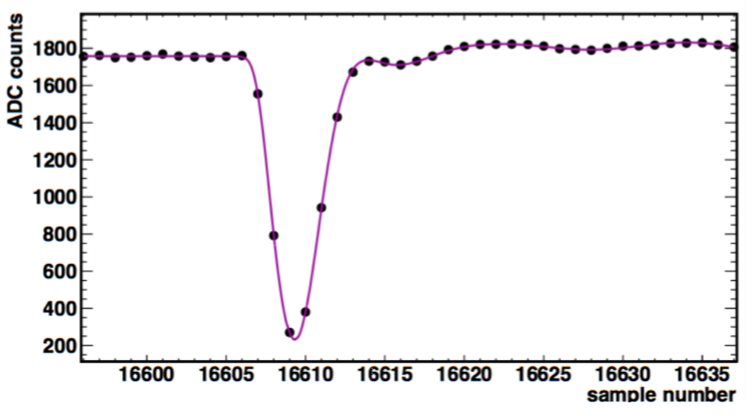
\includegraphics[width=0.6\textwidth]{TemplateFit}
    \caption[Template fit to SiPM trace]{A template fit in purple to a SiPM trace delineated by the black points which is in units of ADC counts. Plot courtesy of Aaron Fienberg.}
    \label{fig:TemplateFit}
\end{figure}


Once a pulse has been fit with a template, the pulse area needs to be converted to real energy units using an energy calibration procedure. A couple of different techniques exist that can be used, including a method that counts photo-statistics seen in the SiPMs \cite{AFThesis}. The default method used is a comparison of lost muon energy signatures in the calorimeters. As described in \refref{lostmuons}, muons lost from the storage ring can spiral inward and hit consecutive calorimeters with a specific time separation between calorimeter hits. These lost muons are minimum-ionizing particles, and thus leave a very distinct energy signature in the crystals, see \secref{sec:lostmuons}. Selecting on the time signature allows hits corresponding to lost muons to be isolated, and the energy signature can be used to determine the appropriate conversions from area to energy\footnote{Different channels can also be equalized based on the energy signatures.}. 


The energy calibration for positron hits as compared to lost muon hits then needs to be determined. Again there are a couple of different techniques, including a comparison of endpoint energies for high energy positrons which tail off at the magic momentum of $\SI{3.094}{\GeV}$, and comparison with simulation. The default technique is to calibrate the energies such that the optimal energy threshold for the \wa analysis is near $\SI{1.7}{\GeV}$ \cite{AFThesis}. Ultimately the energy calibration doesn't matter too much because it is not the energy units that really matter. What really matters is the number of positrons above some energy threshold, where that threshold can be optimized empirically. In fact, the entire \wa analysis could be done without even considering the energy of the incident positrons, and only considering the area of the SiPM pulses\footnote{This statement ignores the effects of pileup which must be accounted for, and applies for a threshold style analysis, and not for other analysis methods which depend on the energy of the pulses.}.


Each pulse fit now has an associated energy and time. Because the measurement of \wa depends heavily on the time reconstruction since the analysis is a frequency extraction, pulse times need to be corrected for various effects in order to reach the precision goal. The fitted times for each pulse need to be aligned on a fill-by-fill basis relative to the injection time of the beam, corrected for any channel differences due to differing pulse shapes or fiber lengths, and corrected for any calorimeter time misalignments due to the use of different laser system components. The fill-by-fill alignment is corrected for using the T0 detector as described in \secref{sec:T0}. The channel differences are corrected by aligning calorimeter channels in time using signals from islands with large simultaneous pulses in neighboring crystals. Calorimeters are time aligned using lost muon coincident events as described before. Once the times of the pulse fits or crystal hits have been determined, the energies can be corrected appropriately for gain effects measured by the laser system. As described in \secref{sub:LaserCalibrationSystem}, the laser calibration system corrects for out-of fill, STDP, and in-fill gain effects, in that order. \figref{fig:IFGFunction} shows an in-fill gain function fit to data for a single calorimeter. Systematic effects for corrected gain effects are studied in \secref{sub:gainerror}.

\begin{figure}[]
    \centering
    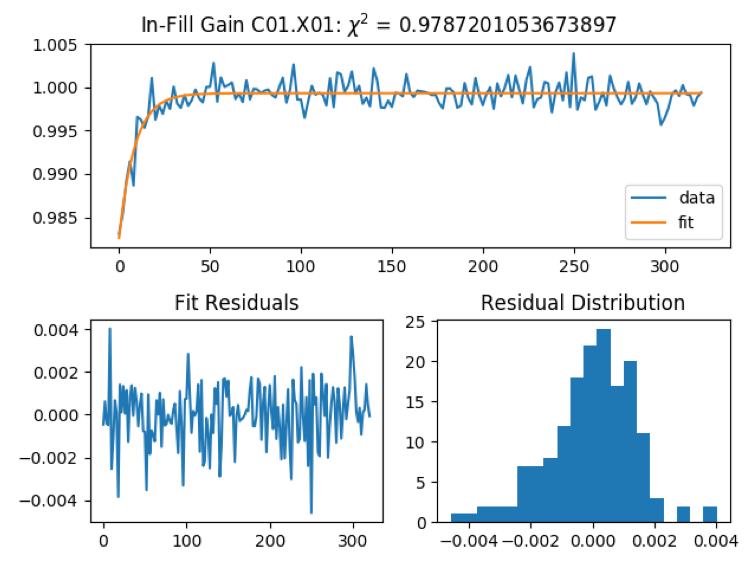
\includegraphics[width=0.6\textwidth]{IFGFunction}
    \caption[In-fill gain function fit for a single calorimeter crystal]{In-fill gain function fit for a single calorimeter crystal (top) and fit residuals (bottom). Each crystal has its own in-fill and STDP gain function parameters. Plot courtesy of Matthias Smith.}
    \label{fig:IFGFunction}
\end{figure}


The last part of the calorimeter reconstruction is the clustering. Clustering is the stage which takes the individual template fit results from separate crystals, and turns them into the times, energies, and positions of decay positron impacts. For a time island with a single positron impact, the procedure is straightforward. The energy for the positron hit cluster is the sum of the individual hit crystal energies. The time for the cluster is taken as the time of the maximum energy hit in the island. This works because most of the deposited energy from a hit is localized to a single crystal. The position of the cluster is determined with a logarithmic weighting function between crystal hits, which for a $\SI{2}{\GeV}$ positron in the E989 calorimeters results in a resolution of $\SI{2}{mm}$ \cite{AFThesis}. See \figref{fig:CaloCluster} for a single calorimeter cluster from a positron hit in the calorimeter. For a time island with multiple positron impacts, the individual crystal hits are separated in time, where the time partitioning separates hits that are $\SI{2.5}{ns}$ apart, and the clustering proceeds as before. For hits which are within this time window, a pileup event has occurred. If the pileup event happens within the same crystal, then the multiple hits are measured as a single hit, and this needs to be corrected for using a pileup subtraction technique, as described in \secref{sub:pileupsubtraction}. For hits that occur in separate crystals, the pileup can be resolved using the spatial separation of the calorimeters. This is an ongoing area of work, and one technique is described in \refref{AFThesis}. For this analysis the spatial separation was turned off, which simplifies the analysis somewhat. This increases the amount of pileup seen in the data, which then needs to be handled by the pileup subtraction technique. For the precision of the Run 1 analysis result, this was found to be acceptable. 


\begin{figure}[]
    \centering
    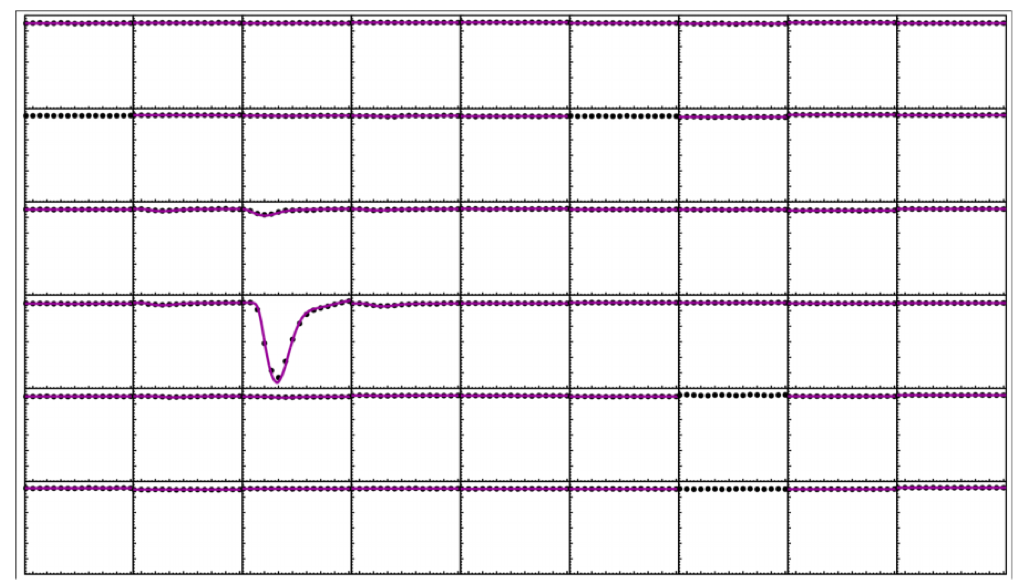
\includegraphics[width=0.9\textwidth]{CaloCluster}
    \caption[Calorimeter cluster from SiPM traces fit with templates]{A single positron hit in the calorimeter, which resulted in a reconstructed calorimeter cluster. Each box is a crystal in the calorimeter, where the contained trace is the SiPM output fit with a template. The positron hit the crystal three from the left and three from the bottom, where it deposited most of its energy. Some of the energy was deposited in the neighboring crystals. Plot courtesy of Aaron Fienberg.}
    \label{fig:CaloCluster}
\end{figure}



\section{Construction of positron hit energy and time spectra}
\label{sec:Histogramming}


Once the reconstruction has processed all calorimeter hits into clusters, the energy and time spectra histograms are made. At the very last stage of the reconstruction procedure, an \textit{art} module takes the produced clusters and puts them into \ROOT \texttt{TTree} formats, where individual data members include the energies, times, calorimeter numbers, etc. of the individual clusters. There is of order 20,000--140,000 cluster data files per dataset, which are combined down to order 200--1,400 \ROOT \texttt{TTree} files. These \ROOT \texttt{TTree}s are then passed through a \ROOT macro to produce \ROOT files with the histograms defined by the \texttt{TH1F} class, one \ROOT histogram file per tree file.


It should be noted that some of the parameter choices for the constructed histograms were informed by analysis results. All analysis parameters were chosen to be identical between the distinct analyzed datasets, in order to simplify both the comparison and combination of different dataset results. This section describes the justification for the different histogram parameters chosen. A table of the histogram parameters is shown in \tabref{tab:histogramparameters}.


\begin{table}[]
\centering
\setlength\tabcolsep{10pt}
\renewcommand{\arraystretch}{1.2}
\begin{tabular*}{.8\linewidth}{@{\extracolsep{\fill}}lc}
  \hline
    \multicolumn{2}{c}{\textbf{Time Spectra Parameters}} \\
  \hline\hline
    Parameter & Value \\
  \hline
    Energy threshold $(E_{th})$ & $\SI{1700}{\MeV}$ \\
    Bin width $(T_{c})$ & $\SI{149.2}{ns}$ \\
    Artifical dead time (ADT) & $\SI{5}{ns}$ \\
    Shadow dead time (SDT) & $\SI{5}{ns}$ \\
    Shadow gap time (SGT) & $\SI{10}{ns}$ \\
    Pileup energy scaling (C) & $1$ \\
    \gmtwo period $(T_{a})$ in Ratio Method & \mus{4.365411} \\
    Muon lifetime (\taumu) in Ratio Method & \mus{64.44} \\
  \hline 
\end{tabular*}
\caption[Parameters used in the construction of \wa time spectra]{Parameters used in the construction of \wa time spectra. \textbf{fill this table out more once I've gone through the various parts}}
\label{tab:histogramparameters}
\end{table}


Energy and time histograms are made for each individual calorimeter. These are summed together to form histograms of all hit times and energies. \figref{fig:energyHist} shows a sample energy spectrum for the Endgame dataset. An energy threshold is applied to the clusters before filling the time histograms. As described at the end of \secref{section:WaIntro}, the optimal energy threshold is where the quantity $NA^{2}$ reaches the maximum, at least in the case of a five parameter fit\footnote{Using the final fit function and looking at the error directly on the fitted \wa frequency, a slightly better estimate can be found.}. By scanning over the choice of energy threshold and fitting the resulting time spectra with \equref{eq:5parfunc}, the optimal energy threshold can be determined as seen in \figref{fig:OptimalEnergyThreshold}. The optimal choice of energy threshold was determined to be $\SI{1700}{\MeV}$, in accordance with the cluster reconstruction energy calibration. 

\begin{figure}[]
    \centering
    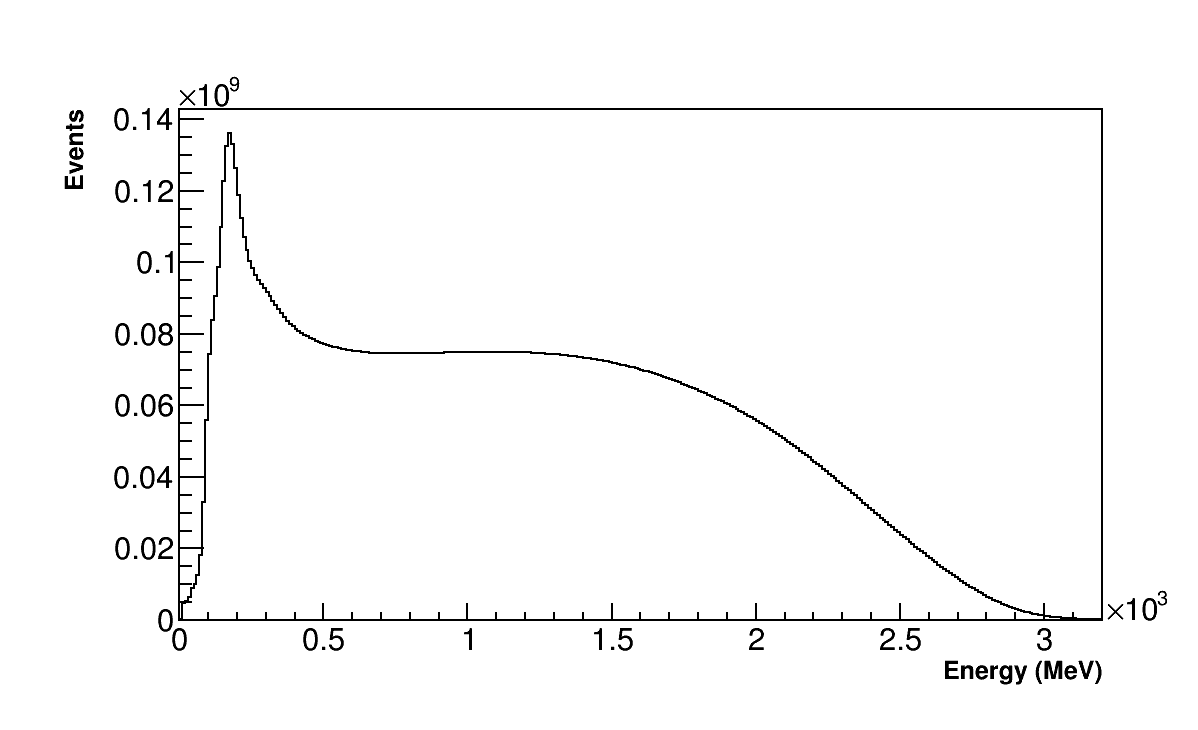
\includegraphics[width=0.7\textwidth]{basicEnergyHist}
    \caption[Sample energy spectrum]{Energy spectrum for hits in all calorimeters for the Endgame dataset on a linear scale. The peak at about 170 \MeV corresponds to lost muons.}
    \label{fig:energyHist}
\end{figure}


\begin{figure}[]
\centering
    \begin{subfigure}[t]{0.45\textwidth}
        \centering
        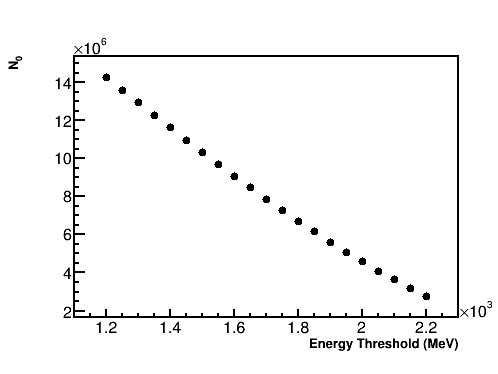
\includegraphics[width=\textwidth]{FiveParameter_N_0_Vs_ETh_9d}
        % \caption{}
    \end{subfigure}
     \begin{subfigure}[t]{0.45\textwidth}
        \centering
        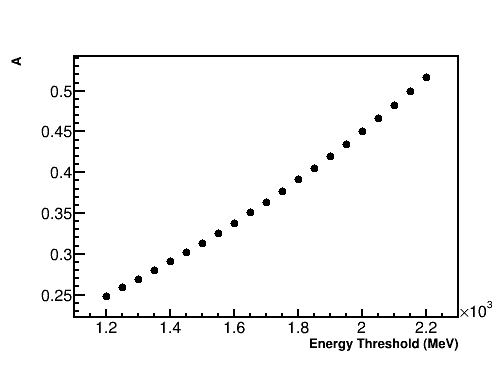
\includegraphics[width=\textwidth]{FiveParameter_A_Vs_ETh_9d}
        % \caption{}
    \end{subfigure}
       
    \begin{subfigure}[t]{0.45\textwidth}
        \centering
        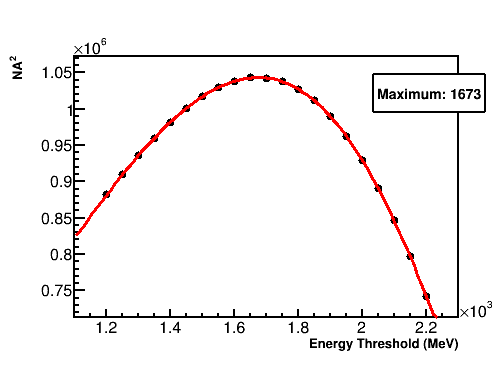
\includegraphics[width=\textwidth]{FiveParameter_NAsq_Vs_ETh_9d}
        % \caption{}
    \end{subfigure}
    \begin{subfigure}[t]{0.45\textwidth}
        \centering
        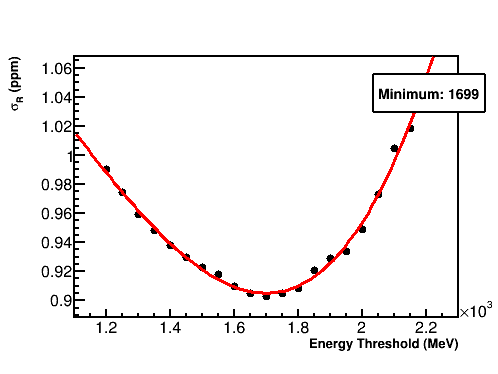
\includegraphics[width=\textwidth]{FullRatio_sigmaR_Vs_ETh_9d}
        % \caption{}
    \end{subfigure}% 
\caption[Determination of optimal energy threshold]{The optimal energy threshold can be determined from the $NA^{2}$ quantity as described in \secref{section:WaIntro} from five parameter fits to the data (bottom-left) or from the calculated error with the final fit function (bottom-right). Fitted $N$ and $A$ parameters are also shown (top) which satisfy Equations~\ref{eq:Nth} and \ref{eq:Ath}. The maximum and minimum are determined using seven parameter polynomial fits to the relevant quantities. The optimal threshold varies slightly per calorimeter and per dataset. Since the region of the minimum is relatively flat, a single energy threshold of 1700 \MeV was chosen. Data from the 9d dataset.}
\label{fig:OptimalEnergyThreshold}
\end{figure}



The optimal bin width for the time histograms was determined to be $\SI{149.2}{ns}$, the average of the cyclotron periods determined from a fast rotation analysis to the data \cite{fastrotationsomething}. As described in \secref{sub:beam_debunching}, this bin width combined with a time randomization on each cluster over a range of $\pm T_{c}/2 = \SI{149.2}{ns} / 2$ serves to eliminate the fast rotation signal in the data\footnote{Some analyzers randomize all times in a single fill by half the cyclotron period as opposed to each individual pulse.}. This randomization is done using \ROOT's \texttt{TRandom3} class. As will be described in \secref{sub:vw_term}, the cluster times are also randomized by the half the vertical waist period, $\pm T_{VW}/2$, where $T_{VW}$ is determined from the inverse of the VW frequency, \equref{eq:VWfreq}. Putting the frequency just in terms of the $n$ value and the cyclotron frequency $f_{c}$ the period is given by
    \begin{align}
        T_{VW} = \frac{1}{f_{VW}} = \frac{1}{(1-2\sqrt{n}) \cdot f_{c}}.
    \end{align}
This randomization is done in order to remove the effects of the VW in the data\footnote{Even though the VW frequency was found to be changing over the course of the fill, this constant time randomization was found to remove all residual traces of the VW in the data.}. The default random seed for each histogram \ROOT file is the hash of the input file name using C++'s standard hash class. Histograms are defined with a time range of 0--\mus{699.8972} (the closest integer multiple of the bin width to \mus{700}), corresponding to 4691 bins. Clusters with times less than \mus{25} or greater than \mus{660} are dropped, corresponding to 4256 bins containing data.



\subsection{Pileup subtraction}
\label{sub:pileupsubtraction}


As described in \secref{sec:Calorimeters}, there will be a certain amount of pileup in the detectors. Pileup again is the term for when multiple particles hit a calorimeter within the dead time of the detector such that they are registered as a single hit or cluster. The measured energy and time spectra for all observed clusters will include this pileup background. For the energy threshold time histogram, the number of counts will be wrong for cases where two below-threshold particles are registered as a single cluster above threshold, and where two above-energy threshold particles are registered as a single cluster. In the former, an extra count is added into the histogram, and in the latter a count is missed. The case where two lower energy positrons are registered as a single higher energy cluster will have a different \gmtwo phase than an actual single cluster at the same energy. This is because the lower energy positrons on average decay from muons which have travelled further around the ring, due to acceptance effects. These muons which have travelled further around the ring have spent more time in the magnetic field, and thus their spins have precessed more. See \figref{fig:PileupExample}. Clusters which originate from pileup events therefore have a different \gmtwo phase than non-pileup events. 


If pileup was a constant effect, then the phase of the time histogram would be shifted by some constant amount, and the extracted \wa frequency would be unaffected. However, the rate of pileup in the detectors changes over the time of a fill, as muons decay away. The rate of double pileup events in the detectors, where the word double indicates cases where two hits are registered as a single cluster, will go approximately as half the rate of single hit events\footnote{It is not exactly half when including the non-linear dead time of the detectors}, and similarly for triple and higher orders of the pileup effect. Because the rate of hits in the detectors oscillates at the \gmtwo frequency, pileup will increase and decrease accordingly leading to oscillations in the pileup time spectra at \wa and 2\wa. The lifetime of the overall pileup effect is approximately half the lifetime at which clusters are registered in the detectors, at \taumu, since double pileup is the dominant contribution. In order to to extract the correct \wa frequency, the pileup effect thus needs to be included in the fit function or subtracted out of the data. The former is challenging due to the non-linear nature of the dead time of the detectors, and would in the end include another phase in the argument of the cosine term in the fit function, thus worsening the statistical precision of the extracted \wa frequency. All analyzers thus construct an approximation of the pileup effect and subtract it from the data before fitting.


% -need to mention the \% level effect of pileup - ~1\% but where do you get that number...


\begin{figure}[]
    \centering
    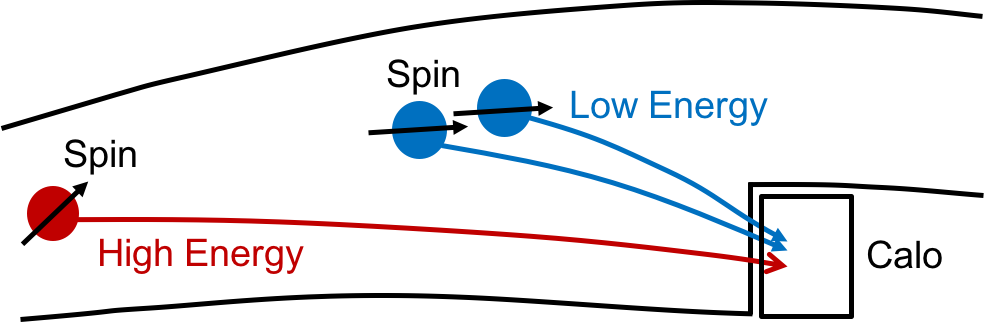
\includegraphics[width=0.5\textwidth]{PileupExample}
    \caption[Pileup example]{Pileup example, where two low energy positrons are registered as a single high energy positron. The black arrows indicate the (exaggerated) direction of the muon spins at the time of decay. Because of acceptance effects the lower energy decay positrons typically come from muons which have traveled further around the ring, and thus the muon spins have precessed more in the magnetic field, leading to a different measured \gmtwo phase for pileup events.}
    \label{fig:PileupExample}
\end{figure}


There are various methods to construct pileup spectra which are then subtracted off the main time and energy spectra. The method used in this analysis is called the `asymmetric shadow method', originally developed in E821 \cite{E821PileupShadow}. This method statistically constructs an approximation for the pileup from the data by assuming that the probability of observing a pileup pulse is the same as the probabilty that two pulses will be offset by some small amount of time, such as \ns{10}. The method works by looking in time windows after trigger pulses to see if a `shadow' pulse exists. If such a pulse exists, then a shadow doublet is created, see \figref{fig:ShadowPileupMethod}. The width of the time window, and the time offset from the trigger pulse to the window, are called the shadow dead time (SDT) and shadow gap time (SGT) respectively. The times and energies of the constructed pileup doublets are taken as
            \begin{gather}
                E_{\text{doublet}} = C \cdot (E_{1} + E_{2}), \label{eq:Edoublet} \\
                t_{\text{doublet}} = \frac{t_{1} \cdot E_{1} + (t_{2}-SGT) \cdot E_{2}}{E_{1} + E_{2}}, \label{eq:tdoublet}
            \end{gather}
where the energy of the doublet is the sum of the two singlet pulses $E_{1,2}$ times some calibration constant $C$, with a default value of 1, and the time of the doublet is the energy-weighted time of the two singlets $t_{1,2}$. The procedure for constructing the pileup spectra is as follows:
\begin{itemize}
    \item{Put each hit into a vector corresponding to a specific fill and a specific calorimeter}
    \item{Time order the hits}
    \item{Loop through the hits, for each hit look within a window of width SDT a time SGT later to see if a shadow pulse exists}
    \item{If a shadow pulse exists, construct a shadow doublet with energies and times as defined in Equations~\ref{eq:Edoublet} and \ref{eq:tdoublet}}
    \item{Randomize $t_{\text{doublet}}$ over the range $\pm T_{c}/2$ (to remove fast rotation as before, \secref{sub:beam_debunching})}
    \item{Per calorimeter, construct pileup energy and time spectra as $P = D - S$, where $D$ is the sum of doublets and $S$ is the sum of singlets used in the construction of the doublets, with the times of the singlets set as $t_{\text{doublet}}$; when constructing the pileup time spectra, only include those doublets and singlets above the energy threshold}
\end{itemize}
Thus pileup energy and time spectra are constructed for each calorimeter, which can then be subtracted off the calorimeter cluster energy and time histograms. When combining the data, the individual pileup histograms are simply added together before subtraction off the calorimeter sum histograms. 


In order to produce an estimate of the pileup spectra which best matches the data, an artifical dead time (ADT) is applied to the data before time randomization. This is done because the true dead time of the detectors depends on the energies and spatial separation of the incoming hits. While this is a small effect, by applying an artificial deadtime and matching the shadow window time, the pileup estimation is improved slightly. The construction of the artificial pileup is handled in the same way as the construction of the shadow pileup, with SGT set to \ns{0}. The constructed artificial doublets replace the singlets in the data. The value for the ADT and SDT is set at \ns{5}, the time threshold at which pileup is 100\% resolved. 

The value of the SGT is simply set to twice the SDT, in order to push the shadow window out to times well beyond the dead time of any pileup events, but not so far that an appreciable fraction of muons have decayed. The value of the doublet energy scaling factor C is set to 1, which is a fine approximation as the spatial separation in the reconstruction is turned off\footnote{With the spatial separation turned off, `pileup' events can occur in crystals that are easily separated by eye. While this increases the level of pileup seen in the data, the pileup approximation method also does not consider the spatial separation, and thus handles the level of pileup accordingly.}. The values for each pileup parameter is shown in \tabref{tab:histogramparameters}. See \secref{sub:pileuperror} for systematic studies on the effect on \wa due to these chosen parameters.



\begin{figure}[]
    \centering
    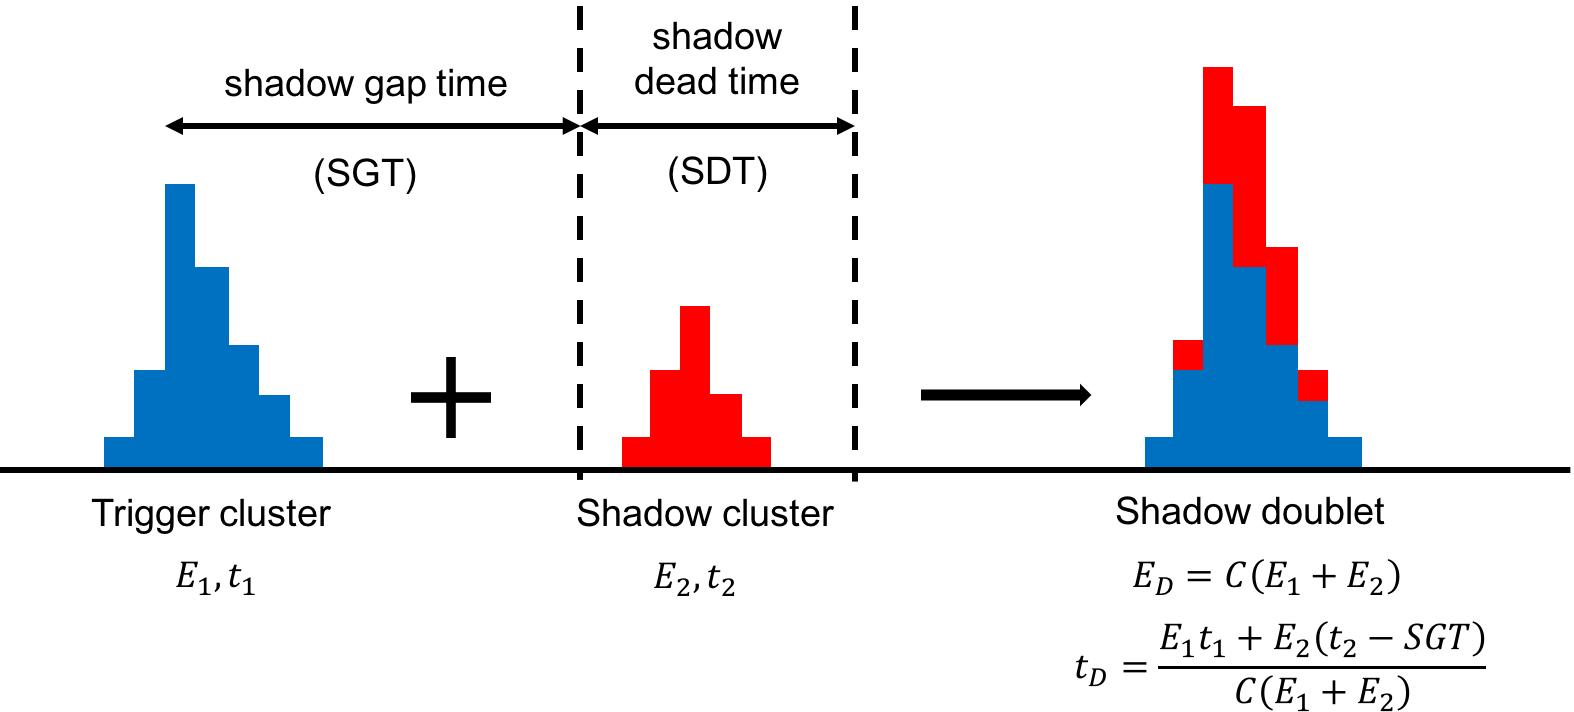
\includegraphics[width=\textwidth]{ShadowPileupMethod}
    \caption[Shadow pileup method]{The shadow pileup method looks for shadow clusters within a time window SDT, a small time away (SGT) from trigger clusters. If a shadow cluster is found, an artificial doublet is formed and included in the pileup spectra if it exceeds the chosen energy threshold.}
    \label{fig:ShadowPileupMethod}
\end{figure}


The pileup energy spectra as compared to the cluster energy spectra is shown in \figref{fig:ClusterEnergiesVsPileupEnergies}. In general, the two lobes starting at approximately $\SI{3}{\GeV}$ and $\SI{6}{\GeV}$ consist of double and triple pileup events respectively\footnote{All orders of pileup fill out the whole energy range, but certain areas consist of mostly one or the other.}. It can be seen that the shadow method of pileup construction produces a pileup energy spectra which is a decent approximation of the cluster energies above the maximum energy that a single decay positron would have at $(\SI{3.094}{\GeV}) + \text{detector resolution}$, for cases of double and even triple pileup. The shape difference arises from two factors: First, the shadow method is only written to construct doublets, and does not consider cases of triple or higher orders of pileup. Second, the real pileup in the data contaminates the construction of the shadow pileup spectra, such that a shadow doublet can be constructed from real pileup pulses. While this alleviates the triplet problem slightly, it means that the doublet pileup spectrum is slightly wrong. The corrected energy spectra (cluster energies minus pileup energies), can be seen in \figref{fig:AddedEnergies}. The shape mismatch is even more apparent as the corrected energy spectrum is high for energies above the expected tail of the true energy distribution, and then goes negative before tailing off to zero. 


    \begin{figure}[]
        \centering
        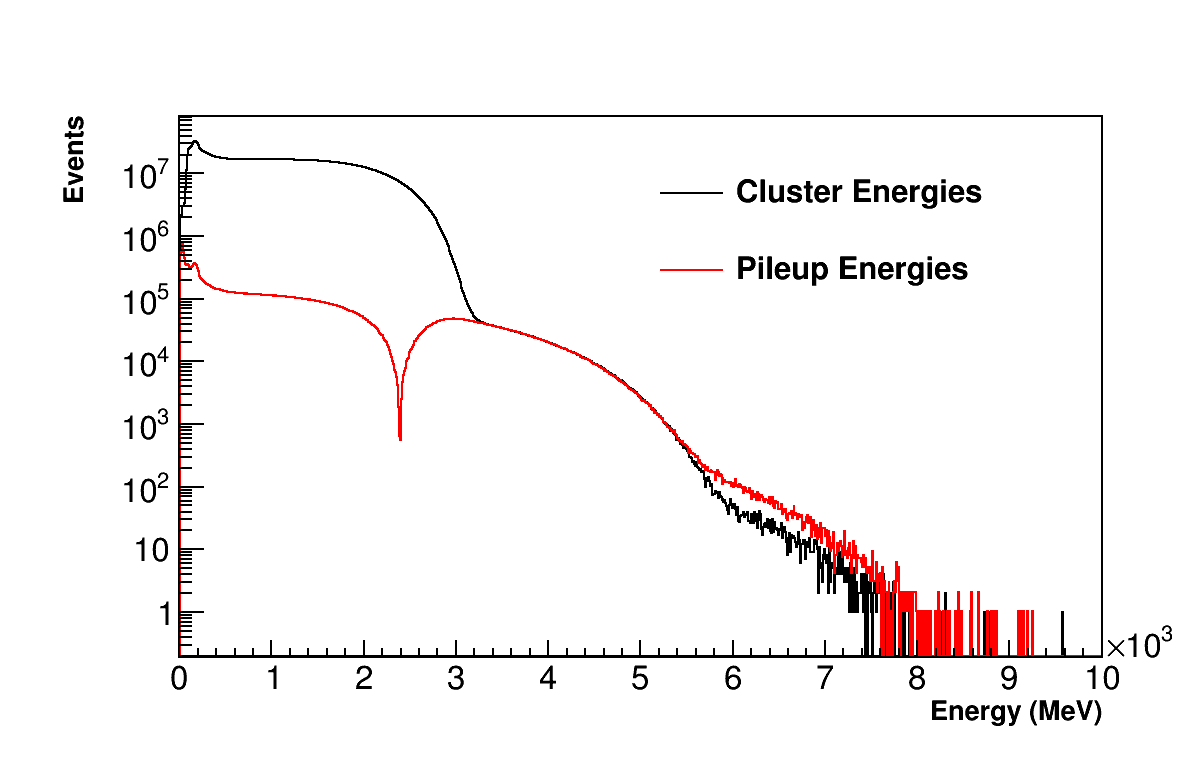
\includegraphics[width=\textwidth]{ClusterEnergiesVsPileupEnergies}
        \caption[Cluster energies vs pileup energies]{Cluster energies in black are plotted vs pileup energies in red, for all calorimeters added together, plotted on a log scale. At energies below about 2.4 GeV the pileup energy spectrum goes negative. In this plot the absolute value of the pileup energies is plotted, and a spike at about 2.4 GeV can be seen as a consequence of this. The shapes do not match perfectly for the constructed pileup spectra, which can be seen at high energies. It should be noted that for energies above $\SI{3.094}{\GeV}$ there is still a shape mis-match even though the red and black curves overlap due to the plotting scale. Data from the 60h dataset.}    
        \label{fig:ClusterEnergiesVsPileupEnergies}
    \end{figure}


    \begin{figure}[]
    \centering
        \begin{subfigure}[]{0.45\textwidth}
            \centering
            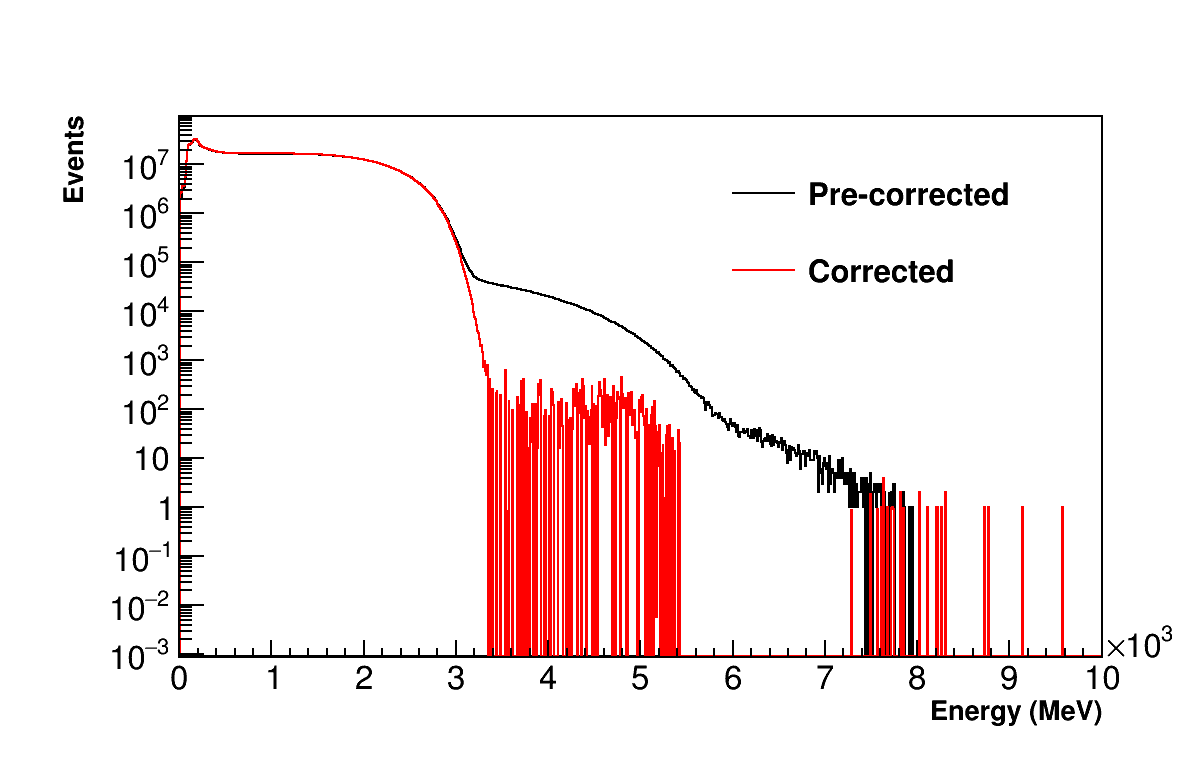
\includegraphics[width=\textwidth]{AddedEnergies}
            \caption{Log scale - the corrected energy spectrum goes negative around 5 GeV.}
        \end{subfigure}% %you need this % here to add spacing between subfigures
        \hspace{1cm}
        \begin{subfigure}[]{0.45\textwidth}
            \centering
            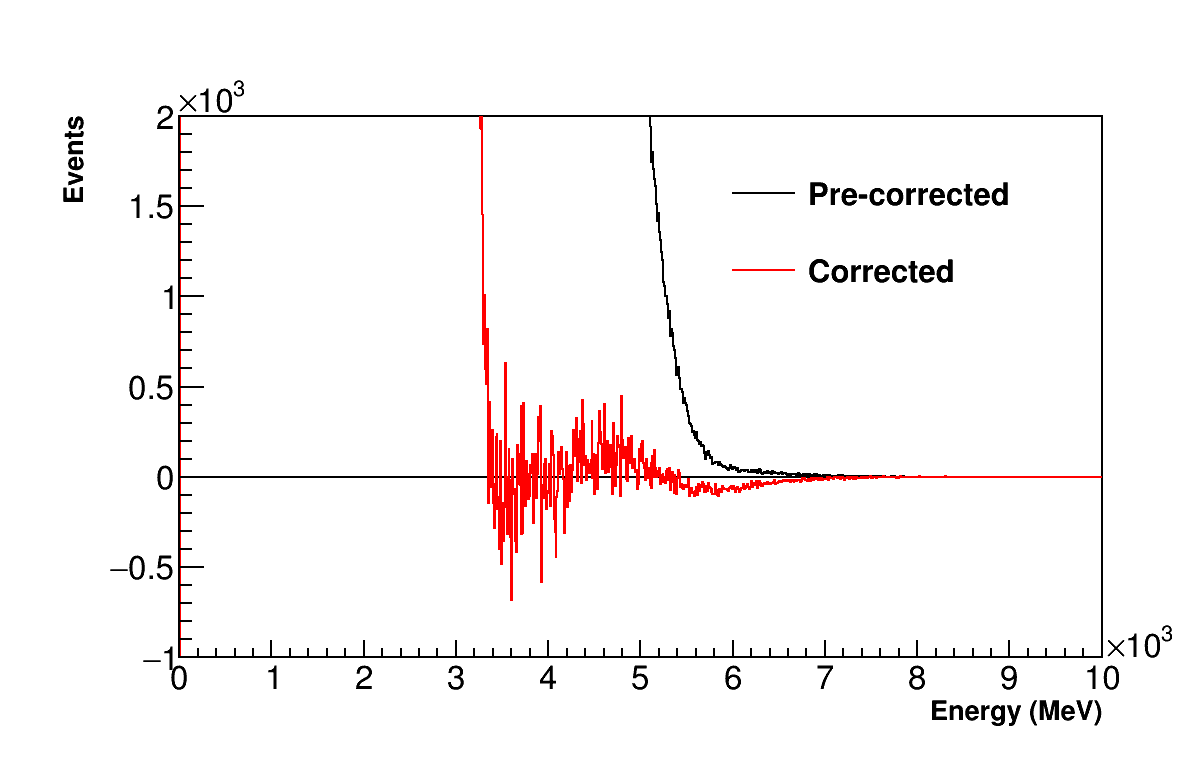
\includegraphics[width=\textwidth]{AddedEnergiesZoomed}
            \caption{Linear scale - zoomed in to show the shape.}
        \end{subfigure}
    \caption[Non-corrected and pileup corrected cluster energies]{Plots for the pre-corrected and corrected energy spectra are shown, all calorimeters added together. Because the triplets and contamination are not accounted for, the corrected energy spectrum does not lie exactly along zero above the energy response of the detectors. Data from the 60h dataset.}
    \label{fig:AddedEnergies}
    \end{figure}



In order to produce a slightly better estimate of the pileup, a multiplier can be applied to the pileup energy and time spectra. By taking the ratio of cluster energies over pileup energies and fitting the region where the energies are dominated by real pileup doublets, a correction factor of approximately 3\% is found, as shown in \figref{fig:EnergyRatio}. Similarly, the cluster times can be examined for cluster energies over \SI{3500}{\MeV}, where the clusters consist purely of pileup pulses, \figref{fig:PileupTimesRatio}. By taking the ratio of the pileup corrected times over all times, the level of residual pileup can be determined. Just as in the ratio of the energies, an approximately 3\% factor is found. When applying this multiplier, the cluster times above \SI{3.5}{\GeV} can be seen to be eliminated as in \figref{fig:PileupTimesRatio}. As will be shown in \secref{sub:pileuperror}, the scale of this multiplier is well within $1\sigma$ of the pileup multiplier error. The final pileup time spectrum for those pileup pulses above energy threshold is shown in \figref{fig:PileupTimeSpectrum}. 


    \begin{figure}[]
        \centering
        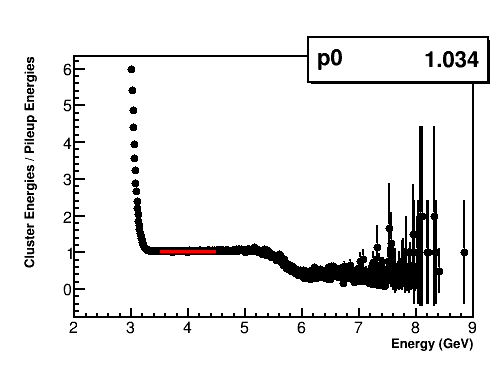
\includegraphics[width=.5\textwidth]{EnergyRatio}
        \caption[Cluster energies divided by pileup energies]{Cluster energies over pileup energies. A region from \SI{3500}{}--\SI{4500}{\MeV} is fit to a straight line, where the doublets dominate the energy distribution. Data from the 9d dataset.}    
        \label{fig:EnergyRatio}
    \end{figure}


    \begin{figure}[]
    \centering
        \begin{subfigure}[]{0.45\textwidth}
            \centering
            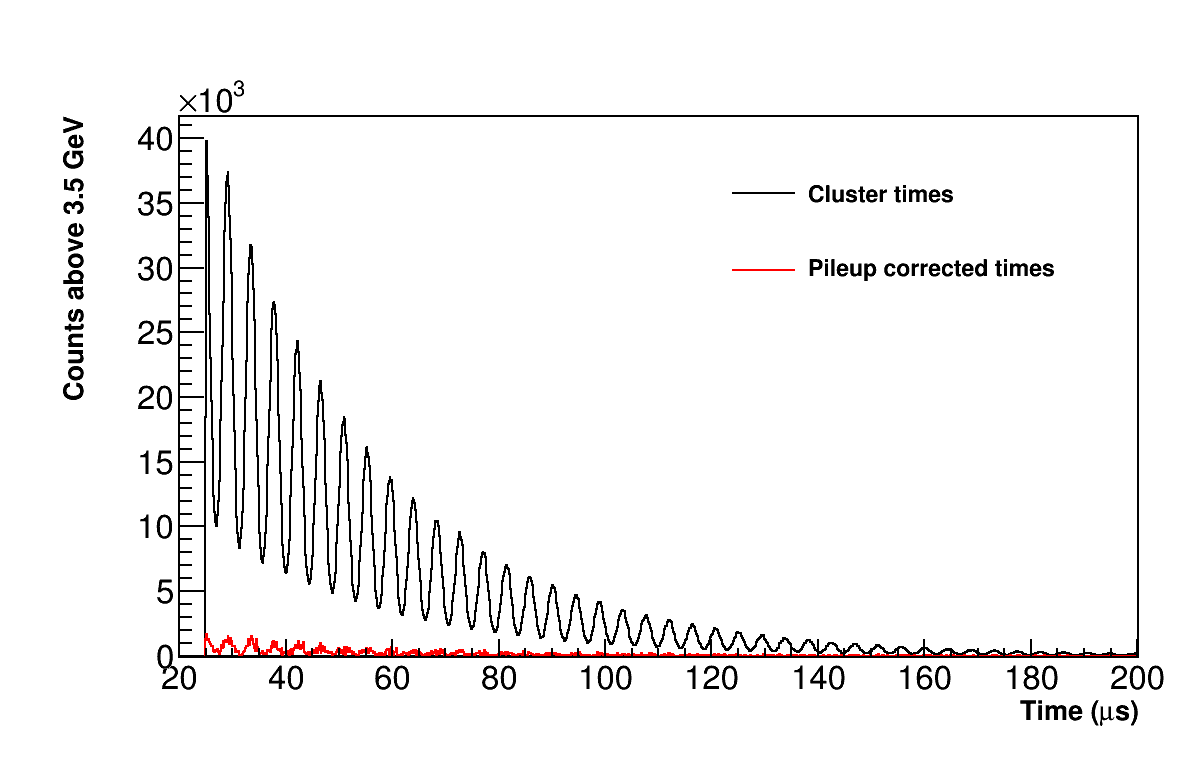
\includegraphics[width=\textwidth]{PileupSubtractedTimesComparison-NoAutoScaling}
            % \caption{Cluster t}
        \end{subfigure}% %you need this % here to add spacing between subfigures
        \hspace{1cm}
        \begin{subfigure}[]{0.45\textwidth}
            \centering
            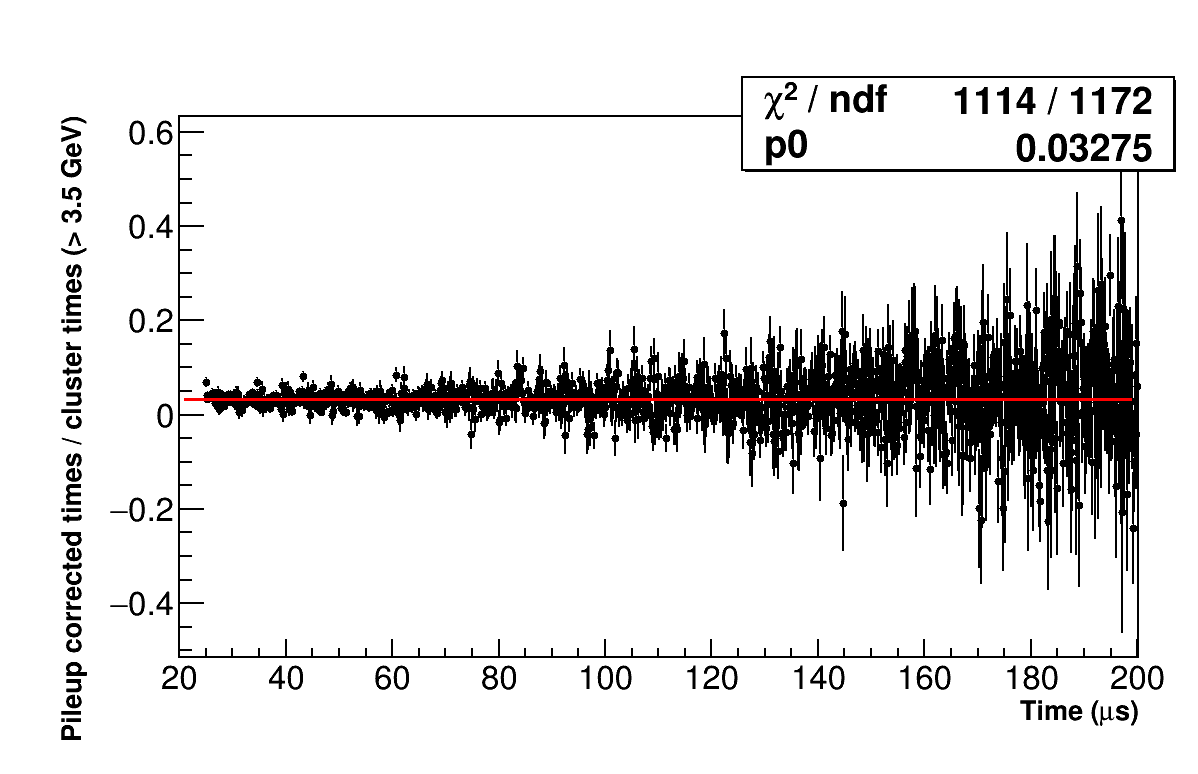
\includegraphics[width=\textwidth]{PileupSubtractedTimesRatio-NoAutoScaling}
            % \caption{}
        \end{subfigure}

        \begin{subfigure}[]{0.45\textwidth}
            \centering
            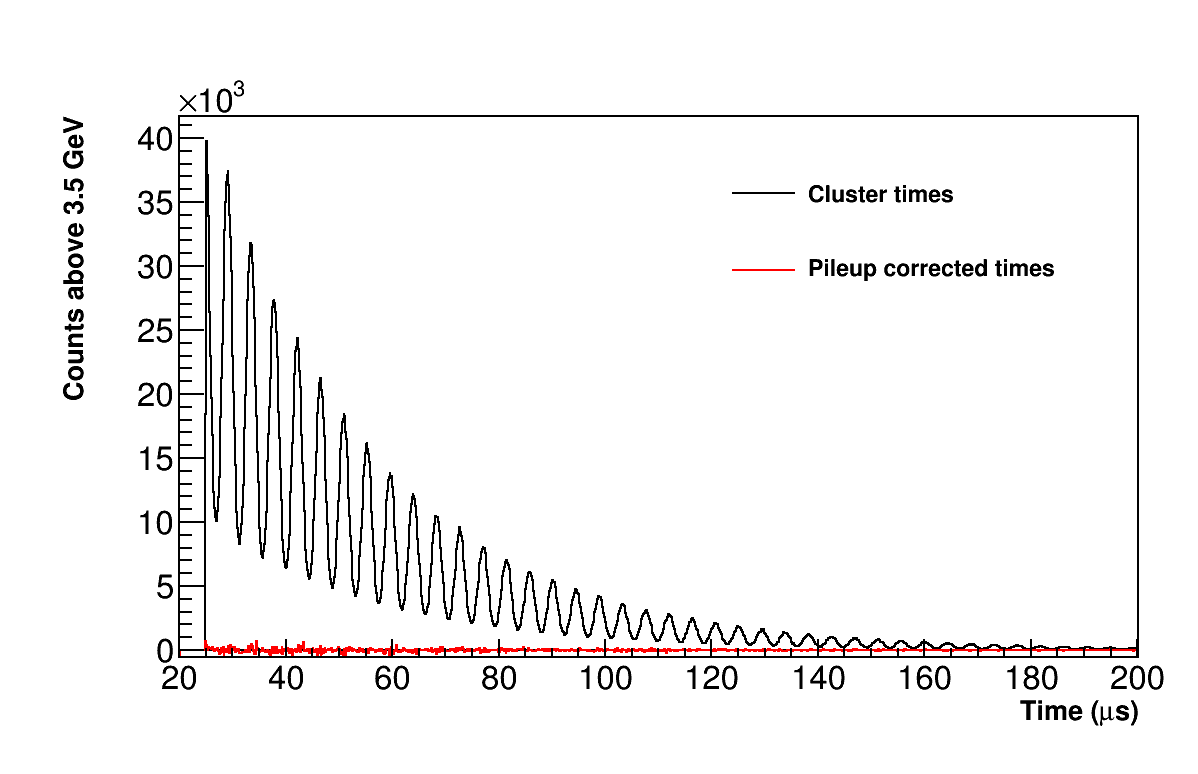
\includegraphics[width=\textwidth]{PileupSubtractedTimesComparison-AutoScaling}
            % \caption{}
        \end{subfigure}% %you need this % here to add spacing between subfigures
        \hspace{1cm}
        \begin{subfigure}[]{0.45\textwidth}
            \centering
            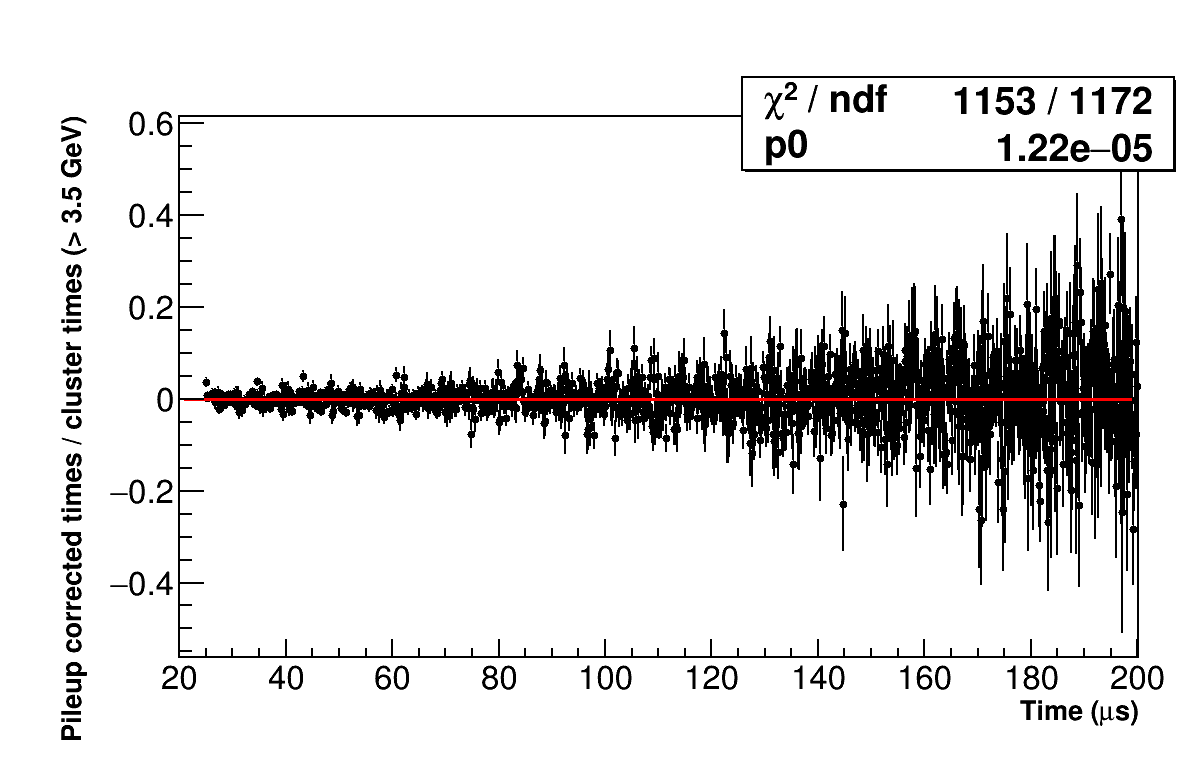
\includegraphics[width=\textwidth]{PileupSubtractedTimesRatio-AutoScaling}
            % \caption{}
        % \label{fig:correctedclustertimes}
        \end{subfigure}
    \caption[Cluster times above \SI{3.5}{\GeV}]{Cluster times and pileup corrected times for counts above \SI{3.5}{\GeV} (left) and their ratio (right). The top two plots are used to determine the approximate level of residual pileup left in the data, coming out to about 3\%. The bottom two plots show the application of that factor and the resulting removal of the remaining pileup. Data from the 9d dataset.}
    \label{fig:PileupTimesRatio}
    \end{figure}



    \begin{figure}[]
        \centering
        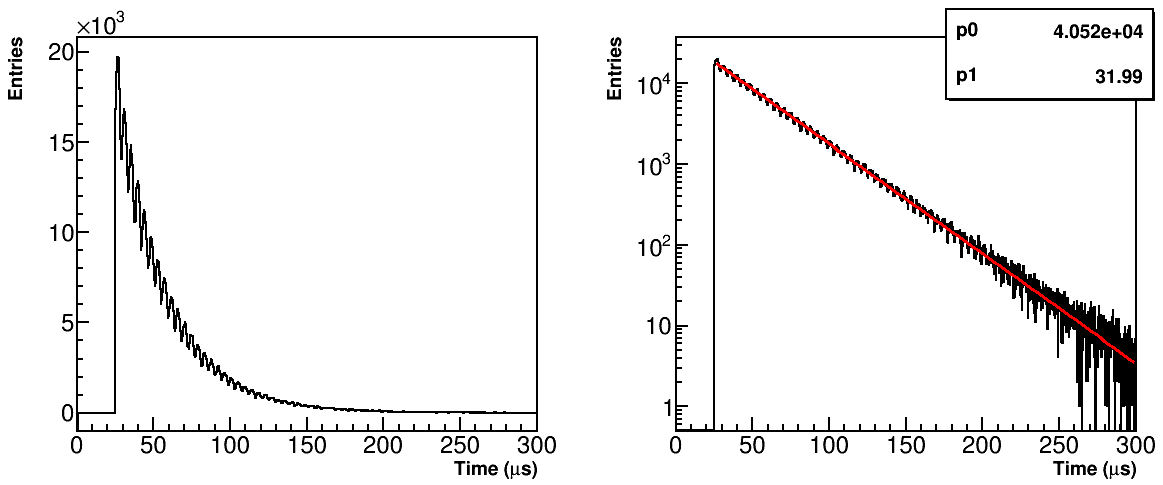
\includegraphics[width=\textwidth]{PileupTimeSpectrum}
        \caption[Pileup time spectrum above threshold]{Plotted is constructed pileup time spectrum on a linear (left) and log (right) scale. The histogram on the right is fit to a simple two parameter exponential to get an idea of the lifetime of the pileup, calculated here as $\SI{31.99}{\micro s}$, which is close to half of the muon lifetime at about $\SI{64.44}{\micro s}$. Data from the 60h dataset.}
        \label{fig:PileupTimeSpectrum}
    \end{figure}





It has been determined that regardless of any residual shape mismatch in the cluster times below \SI{3.5}{\GeV}, the systematic error on the extracted \wa frequency due to the pileup is within the target uncertainty for the level of statistics in the Run~1 dataset, \secref{sub:pileuperror}. For analyses past Run~1 where the error budget is reduced, it may be necessary to improve the shadow method to account for triplets and the contamination. Finally, since the pileup is statistically constructed and then subtracted from the data, the errors on the final time histogram are no longer Gaussian. The proper calculation of the errors is detailed in \appref{app:PileupErrors}.


% https://gm2-docdb.fnal.gov/cgi-bin/private/RetrieveFile?docid=13963&filename=PileupScaleShadowTesting.pdf&version=1
% https://gm2-docdb.fnal.gov/cgi-bin/private/RetrieveFile?docid=14394&filename=PileupFormEtc.pdf&version=2



\subsection{Ratio Method}
\label{sub:ratio_method}

% I put this here because technically the ratio method involves modifying the actual data that is being fit

The method used in this analysis to extract \wa is called the ``Ratio Method,'' or sometimes ``R-Method.'' It is a technique that modifies the data in such a way that the exponential decay in the time histogram is removed, and slow effects are reduced. It was used successfully in the E821 experiment \cite{JKThesis,LDThesis,JPThesis}. A full derivation of the equations in the method is given in \appref{app:RatioDerivation}; here is given a short summary. \figref{fig:RatioFormationFunctions} provides a pictorial representation of how the method works.

The method works by dividing the data into four separate datasets, one with the times of all clusters shifted up by half a \gmtwo period, $+$\Tatwo, one with cluster times shifted down by half a \gmtwo period, $-$\Tatwo, and two unchanged. Assuming the data is described by the five parameter function described in \secref{section:WaIntro} and shown in \figref{fig:fiveparamfunc}, %\equref{eq:5parfunc}
        \begin{align} \label{eq:5parfuncrepeated}
            N_{d}(t, E_{th}) = N_{0}(E_{th}) \cdot e^{-t/\gamma\tau_{\mu}} \cdot [1 + A(E_{th}) \cos(\omega_{a}t+\phi(E_{th}))],
        \end{align}
and that the data is equally split into four subsets, then the new four datasets are given as\footnote{When handling the pileup in the ratio method, the pileup time spectra are split into four datasets and time-shifted in the same way as the cluster hit times. Associated doublets and singlets are kept together in the same individual dataset, and the four pileup datasets are subtracted off their respective ratio datasets before forming the ratio.}:
    \begin{equation}
    \begin{aligned}
        u_{+}(t) &= \frac{1}{4} N_{5}(t+T/2) \\
        u_{-}(t) &= \frac{1}{4} N_{5}(t-T/2) \\
        v_{1}(t) &= \frac{1}{4} N_{5}(t) \\
        v_{2}(t) &= \frac{1}{4} N_{5}(t)
    \end{aligned}
    \end{equation}
In order to time shift the data as such, \Ta needs to be known a priori to high precision. The value used is taken from the E821 result, and its value is taken as $1/f_{a}$, where $f_{a}$ is \SI{0.2290735}{MHz}:
        \begin{align}
            T_{a} \approx \SI{4.365411}{\micro s}
        \label{eq:Ta}
        \end{align}
This value for $f_{a}$ was determined by averaging column 2 of Table XV of the E821 Final Report \cite{E821FinalReport}, which consits of the $f_{a}$ results for the different run periods in that experiment. A systematic error on the choice of this parameter is calculated in \secref{sub:TimeShiftingParameters}.


The datasets are then combined as 
    \begin{equation}
    \begin{aligned}
        U(t) &= u_{+}(t) + u_{-}(t), \\
        V(t) &= v_{1}(t) + v_{2}(t),
    \label{eq:UandV}
    \end{aligned}
    \end{equation}
both of which are shown in \figref{fig:UVfuncs}. It is immediately apparent that the $U(t)$ data are shifted 180\textdegree{} out of phase from the $V(t)$ data. The ratio is then defined as\footnote{The ratio can also be defined with $U(t) - V(t)$ in the numerator, however then the phase of the ratio spectrum is shifted 180\textdegree{} from the original $N_{5}(t)$ spectrum.}
    \begin{align}
        R(t) &= \frac{V(t) - U(t)}{V(t) + U(t)}
    \label{eq:ratioUV}
    \end{align}
where the numerator and denominator are plotted in Figures~\ref{fig:rationumfunc} and \ref{fig:ratiodenomfunc} respectively. The numerator is an exponentially decaying cosine, while the denominator is a simple exponential, both of which can be seen as originating from the difference and sum of the $U(t)$ and $V(t)$ data respectively. The resulting ratio spectrum can be seen in \figref{fig:ratiofunc}, where the exponential has been eliminated. The fit function is then reduced from five parameters down to three:
    \begin{align}
        R(t) \approx A \cos(\omega_{a}t) - C,
    \label{eq:ratiowithC}
    \end{align}
where  
    \begin{align}
        C = \frac{1}{16} \Big(\frac{T}{\tau}\Big)^{2} \approx 2.87 * 10^{-4},
    \end{align}
and these functions have been determined from the time-shifted five parameter function plugged into the $U(t)$ and $V(t)$ variables. In addition to the exponential being eliminated, any slow terms in the data get time-shifted and divided as well, such that the amplitude of said slow effects are reduced. For faster effects, the degree of cancellation of the effect is dependent on the frequency. Effects at frequencies which are an odd multiple of \wa are preserved while effects at an even multiple of \wa are completely cancelled out. An example is shown in \figref{fig:CancellationInRatioMethod}. While this makes fitting the data easier in some cases, in others it is a downside that effects which still need to be included in the fit function now have their amplitudes reduced, making them harder to fit.


    \begin{figure}[]
    \centering
        \begin{subfigure}[t]{0.45\textwidth}
            \centering
            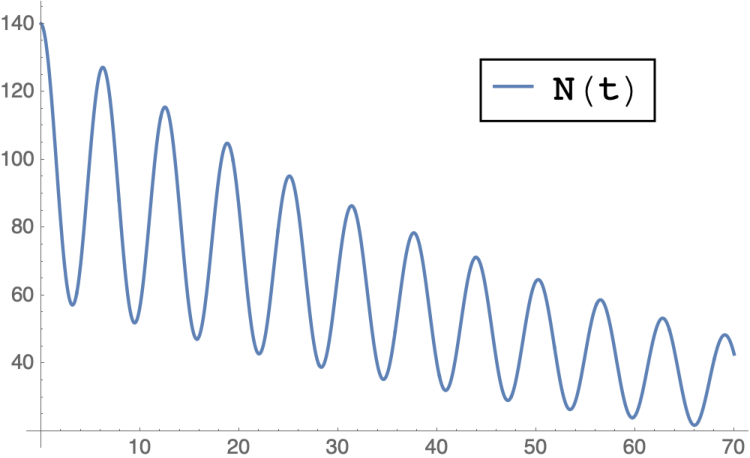
\includegraphics[width=\textwidth]{FiveParamFunc}
            \caption{The five parameter function defined in \equref{eq:5parfuncrepeated}, which describes the incoming data to first order.}
        \label{fig:fiveparamfunc}
        \end{subfigure}%

        \vspace{2mm}
        \begin{subfigure}[t]{0.45\textwidth}
            \centering
            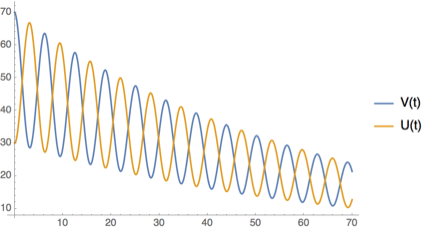
\includegraphics[width=\textwidth]{UVFuncs}
            \caption{$U(t)$ and $V(t)$ functions which describe the time-shifted and unshifted ratio datasets.}
        \label{fig:UVfuncs}
        \end{subfigure}
        \hspace{5mm}
        \begin{subfigure}[t]{0.45\textwidth}
            \centering
            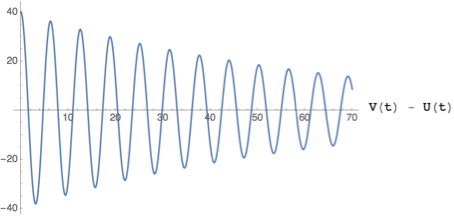
\includegraphics[width=\textwidth]{RatioNumFunc}
            \caption{The numerator function in the formed ratio, $V(t) - U(t)$. It is an exponentially decaying cosine.}
        \label{fig:rationumfunc}
        \end{subfigure}%
        \vspace{2mm}
        \begin{subfigure}[t]{0.45\textwidth}
            \centering
            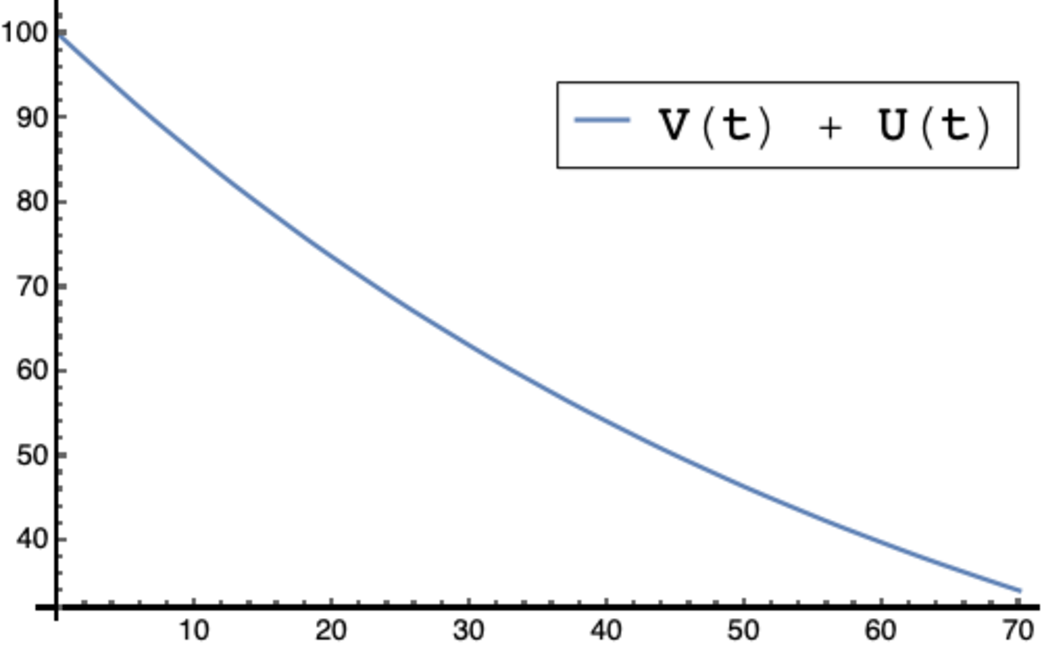
\includegraphics[width=\textwidth]{RatioDenomFunc}
            \caption{The denominator function in the formed ratio, $V(t) + U(t)$. It is an exponentially decaying curve.}
        \label{fig:ratiodenomfunc}
        \end{subfigure}
        \hspace{5mm}
        \begin{subfigure}[t]{0.45\textwidth}
            \centering
            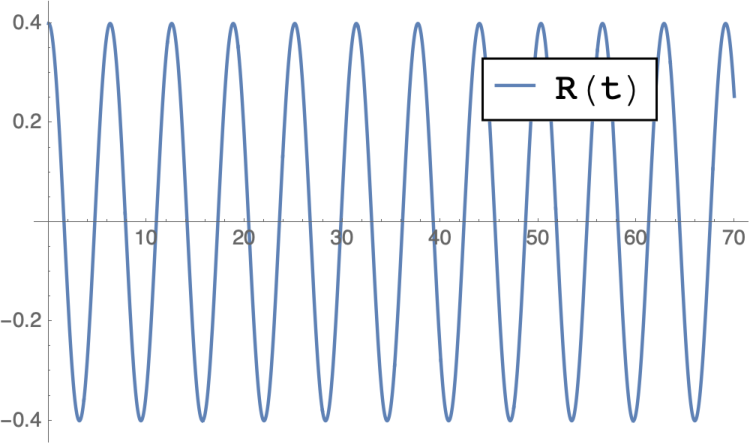
\includegraphics[width=\textwidth]{RatioFunc}
            \caption{The formed ratio function, describing the data after it has been handled as described in the text. To first order it is reduced to a simple cosine form.}
        \label{fig:ratiofunc}
        \end{subfigure}% 
    \caption[Ratio formation functions]{Functions describing the formation of the ratio in the data.}
    \label{fig:RatioFormationFunctions}
    \end{figure}


    \begin{figure}[]
        \centering
        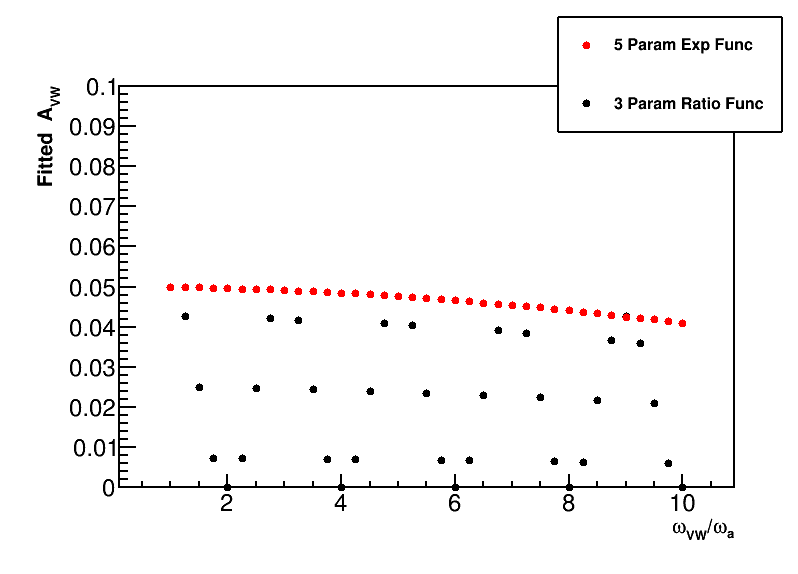
\includegraphics[width=.6\textwidth]{Fitted_Avw_Vs_Wvw_1x-10x}
        \caption[Cancellation of effect in Ratio Method versus frequency]{Fitted amplitude for a VW effect as a function of frequency in units of \wa in a Toy MC simulation, with a five parameter function in red and a three parameter ratio function in black. The input amplitude was 0.05. The fall off of red points is due to the high frequencies relative to the bin widths leading to an underestimate of the amplitude; performing an integral fit removes this trend. As shown the amplitude of the effect goes to zero for frequencies which are an even multiple of \wa.}
        \label{fig:CancellationInRatioMethod}
    \end{figure}



 In order to eliminate the constant $C$ at the end of \equref{eq:ratiowithC}, a different weighting scheme can be used as described in \refref{statisticspaper}:
    \begin{equation}
    \begin{aligned}
        u_{+}(t) &= \frac{e^{T/2\tau}}{2 + e^{T/2\tau} + e^{-T/2\tau}} N_{5}(t+T/2) \\
        u_{-}(t) &= \frac{e^{-T/2\tau}}{2 + e^{T/2\tau} + e^{-T/2\tau}} N_{5}(t-T/2) \\
        v_{1}(t) &= \frac{1}{2 + e^{T/2\tau} + e^{-T/2\tau}} N_{5}(t) \\
        v_{2}(t) &= \frac{1}{2 + e^{T/2\tau} + e^{-T/2\tau}} N_{5}(t)
    \label{eqn:fourHistsInText}
    \end{aligned}
    \end{equation}
Here $\tau = \gamma\tau_{\mu}$, and the factors out front are each close to $1/4$ and account for the degree of muon decay over a time period of \Tatwo. Similar to \Ta, the muon lifetime must be known a priori. It's value is taken as \mus{64.44}, determined from fits to the data. A systematic study regarding this parameter is described in \secref{sub:TimeShiftingParameters}. The ratio spectrum is then almost exactly described by just the cosine term,
    \begin{align} \label{eq:threeparamratio}
        R(t) \approx A \cos(\omega_{a}t),
    \end{align}
in the absence of other effects in the data. 




\section{Fitting the data}
\label{sec:Fitting}


The basic five parameter function used to the fit the data as described before is given as\footnote{In all cases here and onwards the actual fit parameters are in bold.}
    \begin{align}
        f(t) = \boldsymbol{N_{0}} \cdot e^{-t/\boldsymbol{\tau}} \cdot (1 + \boldsymbol{A} \cdot \cos(\omega_{a}t + \boldsymbol{\phi})),
    \label{eq:fiveparfuncagain}
    \end{align}
where the fit parameter for \wa is recast in terms of a ppm level shift \textbf{R} on a reference frequency,
    \begin{align}
        \omega_{a} = 2 \pi \cdot \SI{0.2291}{MHz} \cdot (1 + \textbf{R} \times 10^{-6}).
    \label{eq:wablind}
    \end{align}
This reference frequency of $\SI{0.2291}{MHz}$ was the same reference frequency used in E821, and \textbf{R} is blinded at the hardware and software levels \cite{ClockManual,SoftwareBlinding}. Fitting the data with \equref{eq:fiveparfuncagain} however is insufficient to properly describe the data. \figref{fig:FFT_fiveParameter} shows there are peaks in the FFT due to beam dynamics frequencies corresponding to the CBO, VW, and some beat frequencies with \wa. In order to properly account for these effects, additional terms need to be added to the fit function. 

    \begin{figure}[]
        \centering
        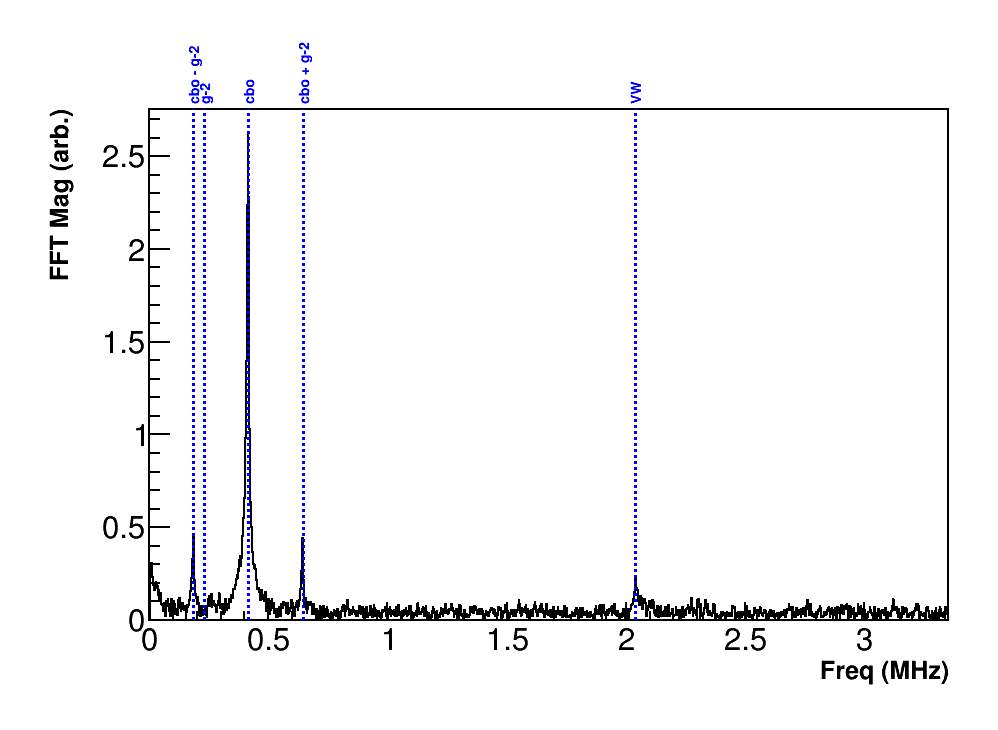
\includegraphics[width=.8\textwidth]{FFT_fiveParameter}
        \caption[FFT of five parameter fit residuals]{FFT of five parameter fit residuals. Peaks corresponding to beam dynamics frequencies of the CBO and VW and some beat frequencies with \wa are readily apparent. A rise at low frequencies corresponds to the effects of the lost muons in the data. The VW peak disappears with the additional level of time randomization at that frequency. From the 60h dataset.}
        \label{fig:FFT_fiveParameter}
    \end{figure}

\equref{eq:fiveparfuncagain} can be expanded to 
    \begin{align}
        f(t) = \Lambda(t) \cdot V(t) \cdot N_{cbo}(t) \cdot \boldsymbol{N_{0}} \cdot e^{-t/\boldsymbol{\tau}} \cdot (1 + A_{cbo}(t) \cdot \cos(\omega_{a}t + \phi_{cbo}(t))),
    \label{eq:TmethodFunction}
    \end{align}
where many additional terms have been added in order to account for effects in the data. The various additional terms $\{N_{cbo}(t), A_{cbo}(t), \phi_{cbo}(t), V(t), \Lambda(t)\}$ are described in the following sections. Fitting the data with this function, referred to as the ``Threshold Method'' or just ``T-Method,'' while not the subject of this dissertation, was done in this analysis as a diagnostic and informative tool for the Ratio Method analysis. 


In order to fit the ratio time spectra as constucted in \secref{sub:ratio_method}, a different function is used. While the immediate inclination is to use an expansion of \equref{eq:threeparamratio} with included additional effects similar to the T-Method fit function, instead the fit function used is a return to the explicit definition of the construction of the ratio time spectra in Equations~\ref{eq:UandV} and \ref{eq:ratioUV}. Including the additional effects previously mentioned, the fit function goes as
    \begin{gather}
        R(t) = \frac{2f(t) - f_{+}(t) - f_{-}(t)}{2f(t) + f_{+}(t) + f_{-}(t)}, \\
        f_{\pm}(t) = f(t \pm T_{a}/2), \\
        f(t) = \Lambda(t) \cdot V(t) \cdot N_{cbo}(t) \cdot (1 + A_{cbo}(t) \cdot \cos(\omega_{a}t + \phi_{cbo}(t))).
    \label{eq:fullratiofunction}
    \end{gather}
The $f(t)$ given here differs from that in \equref{eq:TmethodFunction} in that the $\boldsymbol{N_{0}} \cdot e^{-t/\boldsymbol{\tau}}$ terms have divided out, thus reducing the number of fit parameters necessary to model the data. Using this function as opposed to an expansion of the three parameter ratio function eliminates any approximations made in that three parameter function derivation, and any fit parameters should be consistent in value between the T-Method and Ratio Method results, barring adjustments due to the application of the Ratio Method. 

Because the Ratio Method reduces the sensitivity of the \wa extraction to various effects in the data, peaks that appear in the FFT of the five parameter fit residuals don't appear in the FFT of the three parameter ratio fit residuals, \figref{fig:fft_threeParamRatio}. Indeed except for bad fits, unless one looks at the FFT over the early part of the fit (first \mus{30}) or at the shape of the Ratio Method denominator, one might not know the effects even exist in the data at all. However those effects typically still need to be included in the fit function for a proper estimatation of \wa, and because of the reduction in sensitivity, there are some parameters which the ratio has trouble fitting by itself. Using the T-Method fit function is then a useful tool for constraining these specific parameters.


\begin{figure}[]
\centering
    \begin{subfigure}[t]{0.7\textwidth}
        \centering
        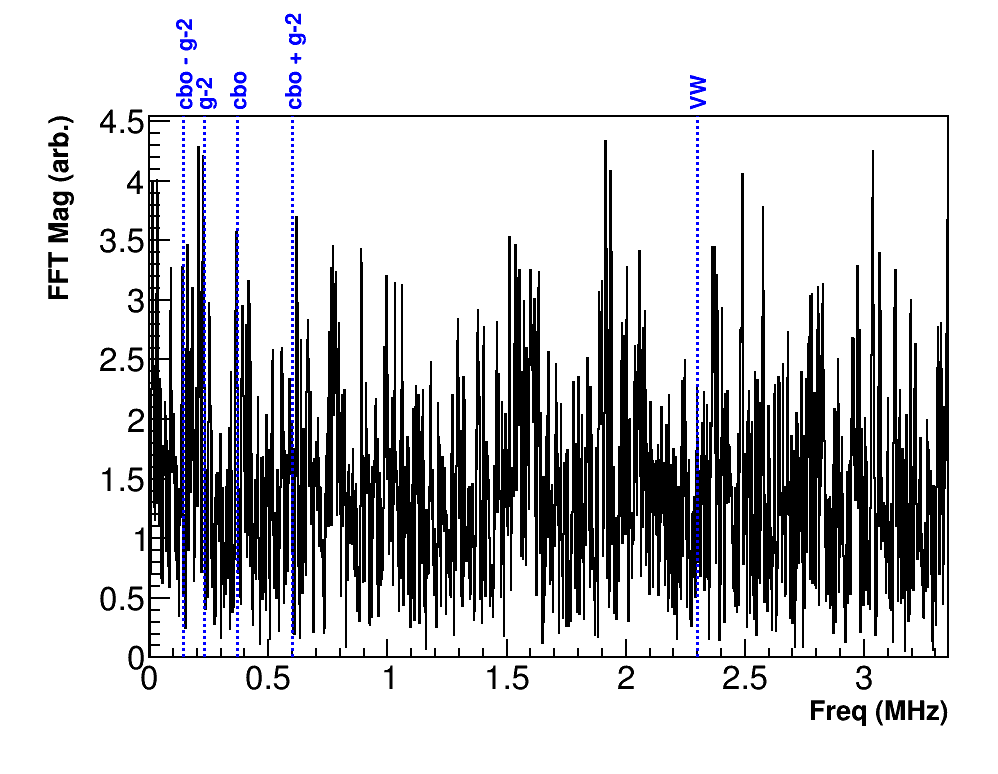
\includegraphics[width=\textwidth]{FFT_threeParRatio_60h}
        \caption{FFT of fit residuals over all times within the fit range. There is no immediately apparent structure for residual effects left out of the fit function.}
    \end{subfigure}%

    \begin{subfigure}[t]{0.7\textwidth}
        \centering
        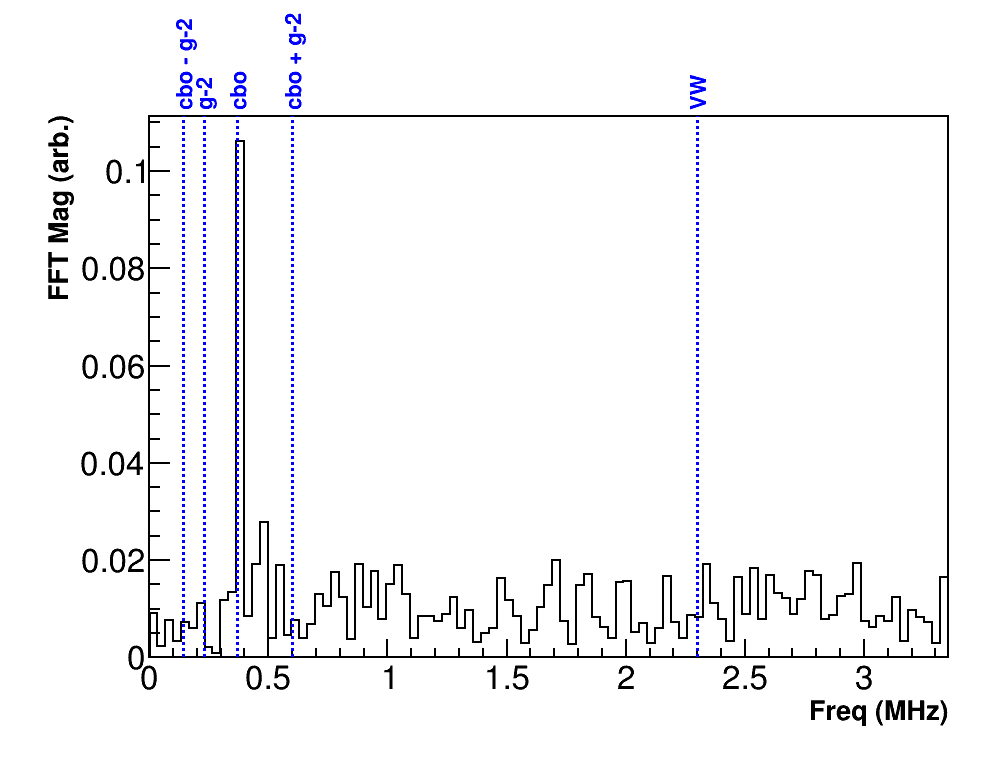
\includegraphics[width=\textwidth]{FFT_threeParRatio_earlyTimes_60h}
        \caption{FFT of fit residuals over the first \mus{30}. The CBO peak can be seen above the noise, though the corresponding beat frequencies do not appear.}
    \end{subfigure}
\caption[FFT of three parameter ratio fit residuals]{FFT of three parameter ratio fit residuals. Dashed blue lines indicate various beam dynamics frequencies and their beat frequencies with \wa. Data from the 60h dataset.}
\label{fig:fft_threeParamRatio}
\end{figure}




\subsection{CBO terms}
\label{sub:cboterms}


As described in \secref{sub:CBO}, the CBO modulates the \wa oscillation. This shows up as a modification on the five parameter function parameters $\{N_{0}, A, \phi\} \rightarrow \{N_{0} \cdot N_{cbo}(t), A_{cbo}(t), \phi_{cbo}(t)\}$ where these terms are given to first order as
    \begin{align}
        N_{cbo}(t) &= (1 + \boldsymbol{A_{cbo-N}} \cdot e^{-t/\boldsymbol{\tau_{cbo}}} \cdot \cos(\omega_{cbo}(t) \cdot t + \boldsymbol{\phi_{cbo-N}})) \label{eq:Ncbo} \\ 
        A_{cbo}(t) &= \boldsymbol{A} \cdot (1 + \boldsymbol{A_{cbo-A}} \cdot e^{-t/\boldsymbol{\tau_{cbo}}} \cdot \cos(\omega_{cbo}(t) \cdot t + \boldsymbol{\phi_{cbo-A}})) \label{eq:Acbo} \\ 
        \phi_{cbo}(t) &= \boldsymbol{\phi_{0}} + \boldsymbol{A_{cbo-\phi}} \cdot e^{-t/\boldsymbol{\tau_{cbo}}} \cdot \cos(\omega_{cbo}(t) \cdot t + \boldsymbol{\phi_{cbo-\phi}}) \label{eq:Phicbo}
    \end{align}
In \equref{eq:Ncbo} the $N_{0}$ term is left out since the ratio fit includes the $N_{cbo}(t)$ term but not $N_{0}$, and in \equref{eq:Phicbo}, $\phi_{cbo}(t)$ has an additive phase instead of a multiplicative one since $\phi_{0}$ is not an amplitude and can be equal to zero. Each of the terms then includes additional fit parameters in an extra amplitude and phase, as well as one shared CBO lifetime and frequency. As described in \secref{sec:MuonBeamMeasurements}, the default model for the CBO modulation is assumed as an exponenetially decaying envelope. The CBO frequency, $\omega_{cbo}(t)$, was time-dependent for Run~1 as found in \secref{sec:MuonBeamMeasurements}. The function for the CBO frequency shown in \figref{fig:CBOFrequency} is given in the fit function as
    \begin{align} \label{eq:CBOfreqForm}
        \omega_{cbo}(t) = \boldsymbol{\omega_{cbo}} \cdot \Big(1 + \frac{Ae^{(-t/\tau_{A})}}{\omega_{0}t} + \frac{Be^{(-t/\tau_{B})}}{\omega_{0}t}\Big),
    \end{align}
where $\boldsymbol{\omega_{cbo}}$ is the free fit parameter, and the model parameters $\{\omega_{0}, A, \tau_{A}, B, \tau_{B}\}$ are fixed from the tracking analysis. These parameters for the various datasets and two tracker stations are given in \tabref{tab:CBOFrequencyParameters}. 



% \begin{landscape}
\begin{table}[]
\centering
\small
\setlength\tabcolsep{10pt}
\renewcommand{\arraystretch}{1.2}
\begin{tabular*}{1\linewidth}{@{\extracolsep{\fill}}lcccccc}
  \hline
    \multicolumn{7}{c}{\textbf{CBO Frequency Model Parameters}} \\
  \hline\hline
    Dataset & Tracker Station & $\omega_{0}$ (rad/\mus{}) & $A$ (rad) & $\tau_{A}$ (\mus{}) & $B$ (rad) & $\tau_{B}$ (\mus{}) \\
  \hline
    \multirow{2}{*}{60h} & 12 & 2.3389 & 2.9 & 81.8 & 5.12 & 7.7 \\
                         & 18 & 2.3387 & 2.82 & 81.1 & 5.08 & 8.2 \\
  \hline
    \multirow{2}{*}{HighKick} & 12 & 2.6145 & 3.27 & 52.8 & 6.96 & 6.6 \\
                              & 18 & 2.6137 & 3.23 & 46.2 & 6.61 & 6.8 \\
  \hline
    \multirow{2}{*}{9d} & 12 & 2.6106 & 2.86 & 72.8 & 5.50 & 8.5 \\
                        & 18 & 2.6110 & 2.89 & 79.2 & 5.44 & 9.2 \\
  % \hline
  %   \multirow{2}{*}{LowKick} & 12 &  &  &  &  &  \\
  %                            & 18 &  &  &  &  &  \\
  % \hline
  %   \multirow{2}{.07\textwidth}{SuperLowKick} & 12 &  &  &  &  &  \\
  %                                             & 18 &  &  &  &  &  \\
  \hline
    \multirow{2}{*}{Endgame} & 12 & 2.3377 & 7.43 & 95.1 & 4.71 & 9.0 \\
                             & 18 & 2.3379 & 7.44 & 95.2 & 4.90 & 9.2 \\                                                        
  \hline
\end{tabular*}
\caption[Dataset CBO frequency model parameters]{Fixed parameters in the CBO frequency model \cite{CBOFreqTrackingElog,JamesPersonalComm}. \textbf{Here I source personal communication with James, as I don't think there's a source for the HighKick numbers.}}
\label{tab:CBOFrequencyParameters}
\end{table}
% \end{landscape}


It should be noted that Equations~\ref{eq:Acbo} and \ref{eq:Phicbo} are not necessarily needed in order to get good fits to the data (whereas \equref{eq:Ncbo} always is). This is typically dataset or random seed dependent. While some datasets had certain parameters with large errors relative to their amplitudes, for this analysis all terms were successfully included in all dataset fits with appropriate tuning of the starting parameters with well converging fits. 


When considering higher order CBO modifications to the fit function, the only term that was found to be fittable was the second order CBO modulation on the $\boldsymbol{N_{0}}$ term, 
    \begin{align}
        N_{2cbo}(t) &= (1 + \boldsymbol{A_{2cbo-N}} \cdot e^{-2t/\boldsymbol{\tau_{cbo}}} \cdot \cos(\omega_{cbo}(t) \cdot t + \boldsymbol{\phi_{2cbo-N}})). \label{eq:N2cbo}
    \end{align}
This stands to reason as the $N_{cbo}(t)$ is the largest CBO effect. The form is assumed to be the same as the first order CBO terms, except the lifetime of the effect is half the CBO lifetime, $\tau_{cbo}/2$. This is due to the fact that the $N_{2cbo}(t)$ is reasoned to come from the width of the oscillating beam, as opposed to the oscillating mean. Indeed as will be shown in \secref{sub:per_calorimeter_fits}, the inclusion of this term is necessary to get good fits to the per calorimeter data, where the CBO effect is stronger compared to in the sum of the calorimeter data. For this reason, and again because the $N_{2cbo}(t)$ term is fittable in the calorimeter sum data, this term is included in fits to each of the datasets.


Systematic studies relating to the choice of envelope and choice of fixed parameters in the frequency model are explored in \secref{sub:cboerror}. For future runs beyond Run~1, it may be necessary to include the higher order modifications to the $\boldsymbol{A}$ and $\boldsymbol{\phi}$ terms.



\subsection{VW term}
\label{sub:vw_term}

As mentioned briefly at the end of \secref{sec:Histogramming}, the VW effect is time-randomized out of the data, such that $V(t) = 1$. This is done due to complications with the Ratio Method. In the 60h and Endgame datasets, the VW frequency was found to be nearly 10 $\cdot$ \wa, on a potential resonance. While to first order this even multiple frequency implies the VW effect should completely cancel out in the Ratio Method, \figref{fig:CancellationInRatioMethod}, the FR effect in combination with the VW leads to a modified envelope for the VW effect in the Ratio Method fits and inflated VW amplitudes \cite{VWinRatio}. See Figures~\ref{fig:VWresonance} and \ref{fig:JamesMC_VW_FR}.

\begin{figure}[]
    \centering
    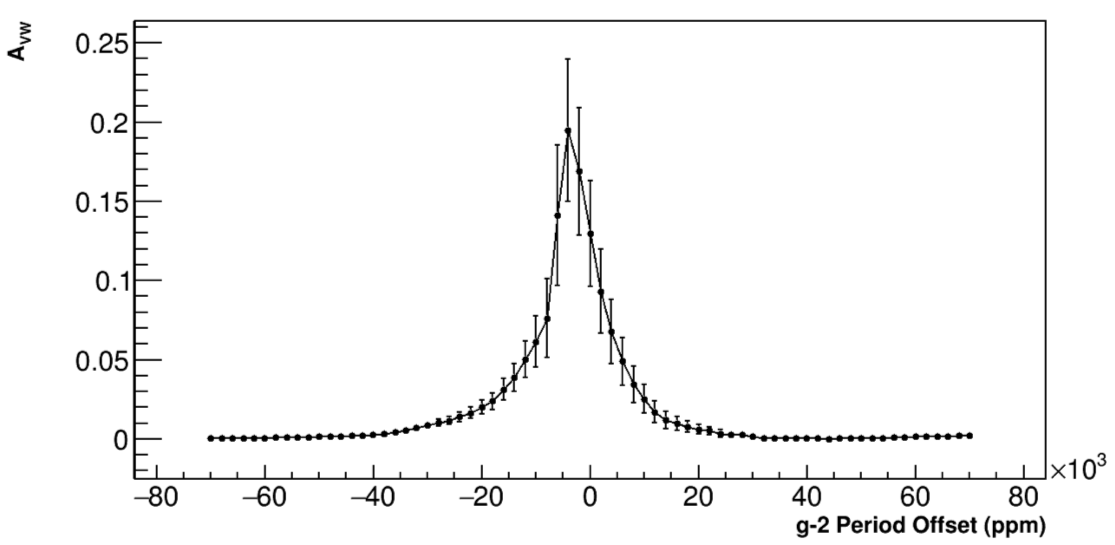
\includegraphics[width=.7\textwidth]{AvwResonance_60h}
    \caption[VW amplitude resonance in the 60h dataset]{Fitted VW amplitude as a function of the choice of  offset from $T_{a}$ in units of thousands of ppm for the 60h dataset. The default time-shift lies at 0 on this plot, right on the resonance where the VW amplitude blows up. Only by time-shifting by a drastically different amount (which negatively affects R), can the resonance be avoided.}
    \label{fig:VWresonance}
\end{figure}


\begin{figure}[]
\centering
    \begin{subfigure}[t]{0.6\textwidth}
        \centering
        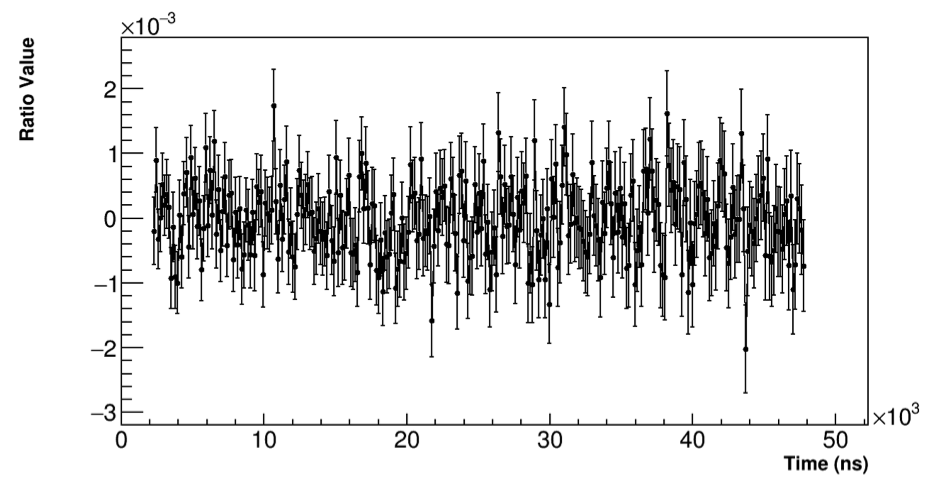
\includegraphics[width=\textwidth]{JamesMC_noFR}
        \caption{Without the FR effect included.}
    \end{subfigure}%

    \begin{subfigure}[t]{0.6\textwidth}
        \centering
        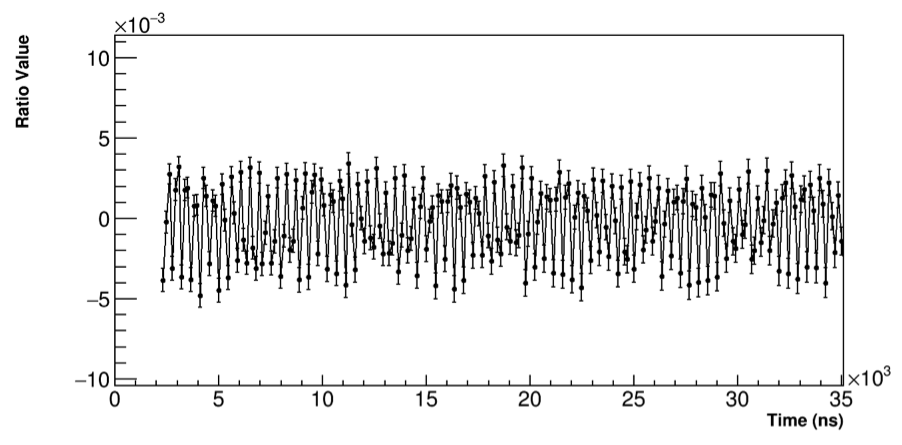
\includegraphics[width=\textwidth]{JamesMC_withFR}
        \caption{With the FR effect included.}
    \end{subfigure}
\caption[VW envelope in Ratio Method Toy MC data with and without FR effect]{Ratio data with and without the FR effect from a Toy MC simulation, with a VW effect with a frequency $\omega_{VW} = 10 \cdot \omega_{a}$. The \wa wiggle itself has been removed, and the lifetime of the VW was set to a large number. The top plot shows ratio data which is consistent with 0 after all effects have been removed and the VW has divided out. The bottom plot shows ratio data inconsistent with 0, with oscillations at the VW frequency, and an interesting beating structure. Note the different scales.}
\label{fig:JamesMC_VW_FR}
\end{figure}


For the 9d dataset which has a VW frequency that's nearly 9 $\cdot$ \wa and avoids said resonance (and by extension the HighKick), it was found that the Ratio Method flattened out the VW amplitudes as a function of calorimeter number leading to a systematically smaller VW amplitude in the calorimeter sum fit. The simplest solution to remove both of these problems was to randomize out the VW effect entirely. \tabref{tab:A_change} gives the change in asymmetry and corresponding change in the statistical error on R due to this added time randomization for three of the Run~1 datasets. It was found that the added randomization increased the statistical error on R by a negligible amount for the Run~1 analysis. It was also found that the added level of time-randomization changed the mean value of R for many random seed fits to the data by a small amount, statistically consistent without the extra randomization \cite{VWinRatio}. Going forward for the future runs, it may be necessary to include the proper VW envelope in the fits using a functional form of the FR instead of randomizing out the effect.

\begin{table}[]
\centering
\small
\setlength\tabcolsep{10pt}
\renewcommand{\arraystretch}{1.2}
\begin{tabular*}{1\linewidth}{@{\extracolsep{\fill}}lcccc}
  \hline
    \multicolumn{5}{c}{\textbf{Change in Asymmetry due to VW Randomization}} \\
  \hline\hline
    Dataset & $A$ no randomization & $A$ with randomization & $\Delta A$ & $\Delta \sigma_{R}$ (ppb) \\
  \hline
    60h & $0.3697$ & $0.3637$ & $-0.0060$ & $22.7$ \\
    9d & $0.3714$ & $0.3639$ & $-0.0075$ & $18.1$ \\
    Endgame & $0.3747$ & $0.3686$ & $-0.0061$ & $10.7$ \\
  \hline
\end{tabular*}
\caption[Asymmetry values in Run~1 datasets with VW time randomization]{Asymmetry values in three of the Run~1 datasets with and without the VW randomization, and the corresponding change in the statistical error on R. An energy cut of 1700 MeV was applied to the data. The HighKick dataset has the lowest asymmetry and the least statistics, so the increase in the statistical error would be negligible as it is for the other datasets.}
\label{tab:A_change}
\end{table}



Barring the envelope changes in the Ratio Method, here is still given the form for the VW as it is used in the T-Method fits. The form for the VW term is taken identically to the CBO terms, 
    \begin{align} \label{eq:VWterm}
        V(t) = 1 + \boldsymbol{A_{VW}} \cdot e^{-t/\boldsymbol{\tau_{VW}}} \cos(\omega_{VW}(t) \cdot t + \boldsymbol{\phi_{VW}}), 
    \end{align}
with an exponentially decaying envelope, and an additional amplitude and phase parameter. The VW frequency $\omega_{VW}$ is given in \equref{eq:VWfreq}, where it is seen to be dependent on the cyclotron frequency and vertical betatron frequency. Using Equations~\ref{eq:tunes} and \ref{eq:CBOfreq}, the dependence on the CBO frequency is seen as
    \begin{equation}
    \begin{aligned}
        \omega_{VW}(t) &= 2\pi (f_{c} - 2f_{y_{BO}}), \\
                    % &= 2\pi \Big[f_{c} - 2f_{cbo}\sqrt{\frac{2f_{c}}{f_{cbo}}-1}\Big]
                    &= 2\pi \Big(f_{c} - 2f_{cbo}(t)\sqrt{2f_{c}/f_{cbo}(t)-1}\Big),
    \label{eq:VWfreqOne}
    \end{aligned}
    \end{equation}
where $f_{cbo}(t) = \omega_{cbo}(t)/2\pi$ is determined in the tracking analysis as described in \secref{sub:cboterms} and given by \equref{eq:CBOfreqForm}. While \equref{eq:VWfreqOne} is the theoretical frequency for the VW effect, it was found in the tracking analysis that including an adjustment factor on the CBO frequency $f_{cbo} \rightarrow \kappa f_{cbo}$ on the order of about a percent resulted in better agreement with the directly measured VW frequency \cite{cbofrequency,verticalbetatron}. In the fitting function itself, the VW frequency is then taken as
    \begin{align} \label{eq:VWfreqKappa}
        \omega_{VW}(t) = 2\pi \Big(f_{c} - 2 \cdot \boldsymbol{\kappa_{VW}} \cdot f_{cbo}(t)\sqrt{2f_{c}/(\boldsymbol{\kappa_{VW}} \cdot f_{cbo}(t))-1}\Big),
    \end{align}
where now the VW frequency fit parameter is $\boldsymbol{\kappa_{VW}}$. The origin of this extra factor is unclear, whether it is a tracker measurement issue, something to do with the frequency function approximation, or if it has something to do with the electrostatic quadrupoles. The inclusion of the extra factor however provides better fits and so it is kept in.




\subsection{Lost muons}
\label{subsec:lostmuons}


Muons lost from the storage ring during the frequency analyis portion of each fill will distort the observed decay positron spectrum. These hits show up as a rise at low frequencies in the FFT of the fit residuals due to the slow nature of the effect, \figref{fig:FFT_fiveParameter}. These muon losses typically originate from those muons with large betatron amplitudes which hit material near the edge of the storage ring, or those muons which experience local field perturbations one too many times. In both cases the muons will lose energy and spiral inward out of the ring, a fraction of which will then pass through multiple calorimeters. Because lost muons are minimum-ionizing particles (MIPs), they are relatively easily identified by their small energy deposition signature in hit calorimeters, around 170 \MeV as shown in the left peak in \figref{fig:energyHist}. These lost muons typically have a flight time between adjacent calorimeters of $\Delta t_{12} = \SI{6.5}{ns}$ \cite{lostmuonspaper,lostmuonsDenverTalk}. The $\Delta t$ and energy deposition distributions are shown in \figref{fig:lostmuondistributions}. By looking for coincidences between three adjacent calorimeters, or triples, and then applying cuts and subtracting backgrounds, a pure sample of lost muons can be constructed. This lost muon spectrum $L(t)$ can then be implemented into the fit function in order to account for the positrons that would have been observed in the absence of losses.

\begin{figure}[]
\centering
    \begin{subfigure}[]{0.48\textwidth}
        \centering
        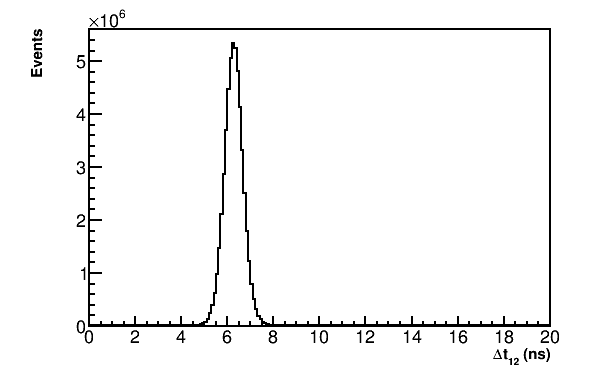
\includegraphics[width=\textwidth]{triples_deltaT_Endgame}
        \caption{}
    \end{subfigure}% %you need this % here to add spacing between subfigures
    \begin{subfigure}[]{0.48\textwidth}
        \centering
        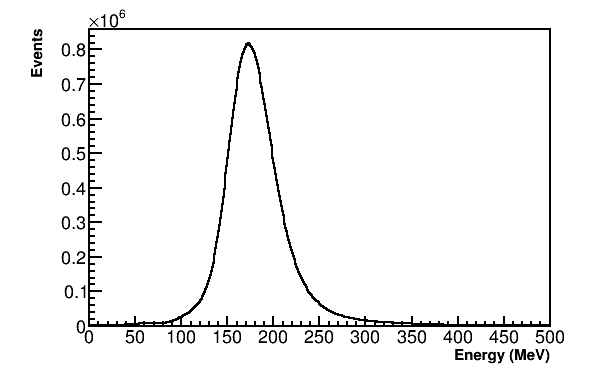
\includegraphics[width=\textwidth]{triples_Edep_Endgame}
        \caption{}
    \end{subfigure}
\caption[Lost muon $\Delta t$ and energy deposition distributions]{$\Delta t$ and energy deposition distributions for lost muons passing through adjacent calorimeters. A typical flight time is \ns{6.5} and energy deposition is 170 \MeV. Data from the Endgame dataset.}
\label{fig:lostmuondistributions}
\end{figure}


\begin{table}[]
\centering
\setlength\tabcolsep{10pt}
\renewcommand{\arraystretch}{1.2}
\begin{tabular*}{1\linewidth}{@{\extracolsep{\fill}}lc}
  \hline
    \multicolumn{2}{c}{\textbf{Lost Muon Cuts}} \\
  \hline\hline
    Parameter & Value or Range \\
  \hline
    Cluster size & $\leq$ 3 crystals \\
    Cluster energy fraction & $\geq$ 0.8 in main crystal \\
    Time of flight between adjacent calorimeters & $\SI{5}{ns} \leq \Delta t_{12, 23} \leq \SI{7.5}{ns}$ \\
    Energy deposition & $\SI{100}{\MeV} \leq E_{1,2,3} \leq \SI{250}{\MeV}$ \\
    Time of flight between separated calorimeters & $\Delta t_{13} \leq \SI{14.4}{ns}$ \\
  \hline 
\end{tabular*}
\caption[Lost muon cuts]{Lost muon selection cuts. In a triple coincidence the subscripts of 1, 2, and 3 correspond to the three calorimeters hit clockwise around the ring.}
\label{tab:lostmuoncuts}
\end{table}



The cuts used for the lost muon selection are given in \tabref{tab:lostmuoncuts}. Triple coincidences are only included where every cluster consists of three or less crystals hit, with 80\% of the energy deposited in one crystal. $\Delta t$ and energy deposition ranges are taken as $\SI{5}{ns} \leq \Delta t_{12, 23} \leq \SI{7.5}{ns}$ and $\SI{100}{\MeV} \leq E_{1,2,3} \leq \SI{250}{\MeV}$, where these ranges come from inspection of \figref{fig:lostmuondistributions}. The \DT distribution as a function of time in-fill is shown in \figref{fig:deltaT12_AccSub}. By examining this distribution in the range $\SI{2}{ns} \leq \Delta t_{12} \leq \SI{4}{ns}$, and averaging the contained counts, an approximation for the accidental background can be determined and subtracted off the triples spectrum. The accidental background typically comes from either double coincidences and a real positron hit, or a particle shower induced by an incident positron which hits an adjacent calorimeter. 


% \begin{figure}[]
% \centering
%         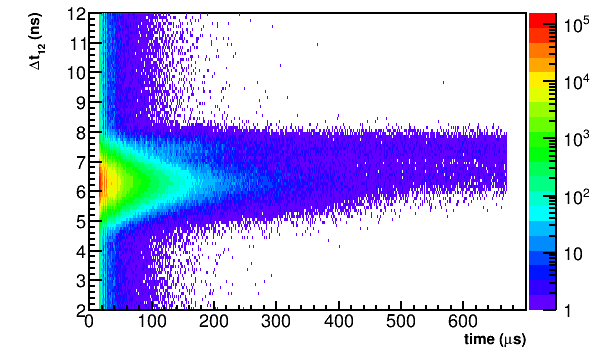
\includegraphics[width=0.9\textwidth]{deltaT12_beforeAccSubtraction_Endgame}
%         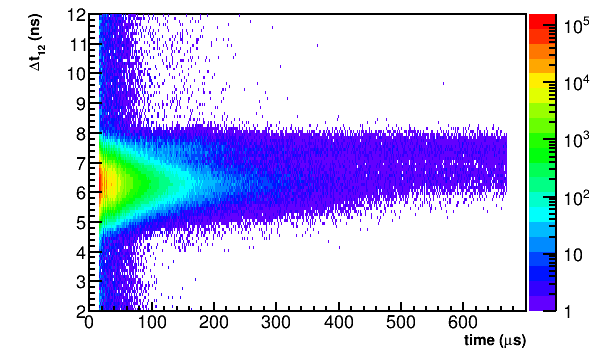
\includegraphics[width=0.9\textwidth]{deltaT12_afterAccSubtraction_Endgame}
% \caption[Lost muon \DT distribution as a function of time in-fill]{\DT distribution as a function of time in-fill before (top) and after (bottom) accidental background subtraction. Note the log scale and the cahnge in colors at the far left of the bottom plot. Lost muons have a \DT distribution centered at \ns{6.5}. The accidental background can be seen as counts out at $\Delta t$'s far from the center of the distribution. Color striations in the core of the distribution correspond to CBO periods. There are two bands of hits that do not fall off as severely with time as the lost muons do. The band contained between 7 and \ns{8} corresponds to deuterons, while the band contained between 6 and \ns{7} corresponds to protons. Data from the Endgame dataset.}
% \label{fig:deltaT12_AccSub}
% \end{figure}

\begin{figure}[]
\centering
        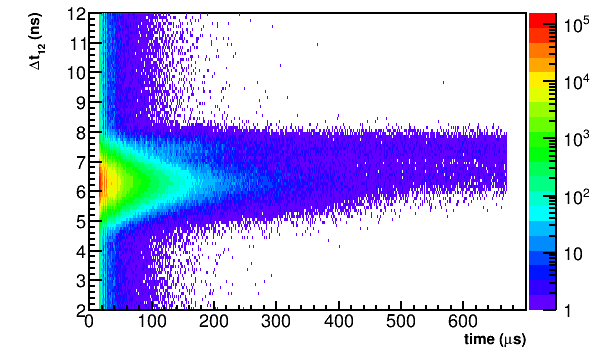
\includegraphics[width=1\textwidth]{deltaT12_beforeAccSubtraction_Endgame}
\caption[Lost muon \DT distribution as a function of time in-fill]{\DT distribution as a function of time in-fill before any cuts. Note the log scale. Lost muons have a \DT distribution centered at \ns{6.5}. The accidental background can be seen as counts out at $\Delta t$'s far from the center of the distribution. Color striations in the core of the distribution correspond to CBO periods. There are two bands of hits that do not fall off as severely with time as the lost muons do. The band contained mostly between 7 and \ns{8} corresponds to deuterons, while the band contained mostly between 6 and \ns{7} corresponds to protons. Data from the Endgame dataset.}
\label{fig:deltaT12_AccSub}
\end{figure}


Also shown in \figref{fig:deltaT12_AccSub} are two bands of stable beam contaminants corresponding to stored deuterons and protons. These particles have different times of flights between calorimeters due to their larger masses. By looking at the $\Delta t_{13}$ distribution for times greater than \mus{300}, the deuteron population is easily isolated, \figref{fig:deuteronPop}. While the deuteron population is mostly removed by the \DT cut, an additional cut of $\Delta t_{13} \leq \SI{14.4}{ns}$ helps remove any remaining deuteron contamination. The proton population, due to it's nearness to the real lost muon population, is harder to remove. The simplest solution is to simply cut on the negative side of the \DT or $\Delta t_{13}$ distributions. See \secref{sub:lostmuonserror} for the results using this additional cut. It was found that the proton contamination makes almost no difference to the fitted value of R. The default choice then is to use the previously specified cut ranges in order to increase the amount of statistics in the lost muons distribution with which to fit. A study into the exact rate of these beam contaminants is included in \refref{lostmuonsKevin}.


\begin{figure}[]
    \centering
    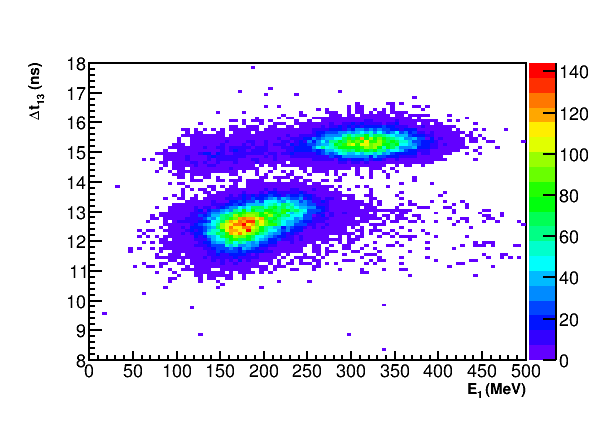
\includegraphics[width=.7\textwidth]{deuteron_Population_Endgame}
    \caption[Deuteron population at late times]{$\Delta t_{13}$ distribution as a function of energy for times greater than \mus{300}. The lost muons can be seen as a blob centered at 170 \MeV and $\Delta t_{13} \approx \SI{12.5}{ns}$, while the deuterons can be seen as the oblong blob at $\Delta t_{13} \geq \SI{14.4}{ns}$. While the deuterons have a preferentially larger energy deposition, they can be seen to extend to low energies, making cutting on energy unrealistic. Though not easily separated by eye, the stored protons are contained within the upper right portion of the lost muons blob. Data from the Endgame dataset.}
    \label{fig:deuteronPop}
\end{figure}


The last background is the quadruples spectrum. Due to how the triple coincidences are constructed, real quadruples will be counted as two separate triples. While the quadruples spectrum can be used instead of the triples spectrum for a purer sample of lost muons, the amount of statistics is much reduced, and similarly for higher order coincidences. The quadruples spectrum is constructed in the same was as the triples with the same cut ranges. The quadruple background is removed by subtracting off those triples which originated from quadruple coincidences.


\begin{figure}[]
    \centering
    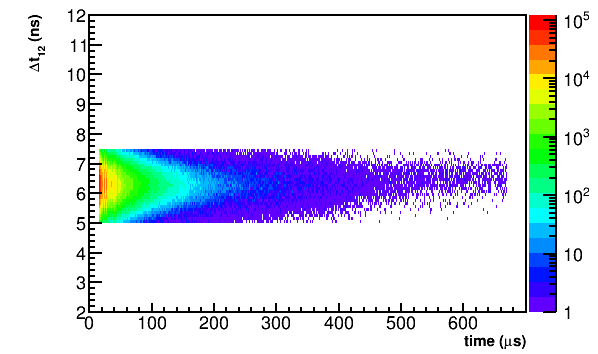
\includegraphics[width=.8\textwidth]{deltaT12_timeInFill_finalCuts_Endgame}
    \caption[Final \DT distribution for selected lost muons]{Final \DT distribution for selected lost muons as a function of time in-fill. Data from the Endgame dataset.}
    \label{fig:finalDT12Dist}
\end{figure}

\begin{figure}[]
    \centering
    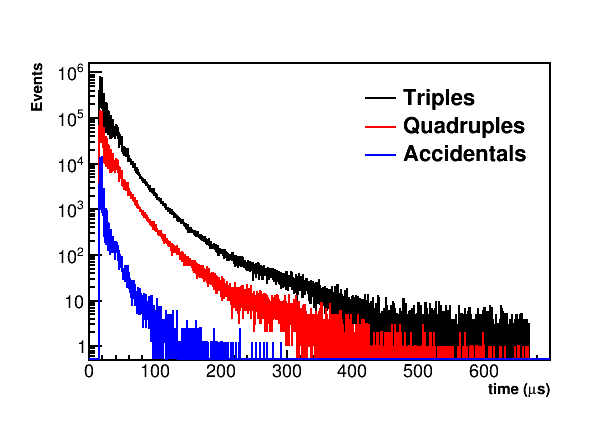
\includegraphics[width=0.9\textwidth]{Triples_vs_all_Endgame}
    \caption[Lost muon triples spectrum compared to quadruples and accidental background]{Lost muon triples spectrum $L(t)$ as a function of time in-fill, after all cuts and background subtractions. Also shown are the quadruples and accidental background distributions, which can be seen to be much smaller than the triples. The shape of the triple and quadruple spectra can be seen to be nearly the same. The shape of the triples spectrum comes from beam dynamics (CBO) and lost muon acceptance effects. Data from the Endgame dataset.}
    \label{fig:triples}
\end{figure}


\figref{fig:finalDT12Dist} shows the final \DT distribution with cuts as a function of time in-fill for selected lost muons. The final 1D triple losses spectrum $L(t)$ is shown in \figref{fig:triples}. Once we have the lost muon distribution we need to include it in the fit function in order to account for the changing number of hits over the course of the fill. The true lost muon rate will be given by $L(t)/\epsilon$, where $\epsilon$ is the loss detection efficiency \cite{AFThesis}. The change in the number of muons within the storage ring can be written as 
    \begin{align} 
        dN = -\frac{N}{\tau} dt - \frac{L(t)}{\epsilon} dt, 
    \end{align}
where the solution can be determined by inspection as
    \begin{align} 
        N(t) = N_{0} \cdot e^{-t/\tau} \cdot (1 - \frac{1}{\epsilon N_{0}} \int_{t_{0}}^{t} L(t')e^{(t'/\tau)} dt').
    \end{align}
The parameter $\tau$ is the same muon lifetime as in the T-Method fit function, except here it is set as the default value of \mus{64.44}\footnote{The fitted \wa frequncy is largely insensitive to this parameter, and especially so in the Ratio Method fits, so this is acceptable.}. The value for $t_{0}$ can be taken as any time at or before the start of the fitting range, as it simply changes the scale of $N_{0}$ which is largely unimportant. The modification $\Lambda(t)$ as listed in \equref{eq:TmethodFunction} is then taken as
    \begin{align} \label{eq:lambdalosses}
        \Lambda(t) = 1 - \boldsymbol{\kappa_{loss}} \int_{t_{0}}^{t} L(t')e^{(t'/\tau)} dt'
    \end{align}
where $\boldsymbol{\kappa_{loss}} = 1/\epsilon N_{0}$ is taken as the fit parameter\footnote{By construction $\kappa_{loss}$ is a very small parameter, $\mathcal{O}(10^{-10})$. This factor is absorbed into the parameter in such that the fit parameter is $\mathcal{O}(1)$.}.

It should be noted that the Ratio Method is largely insensitive to the slow lost muons effect which divides out. No rise appears in the FFT of the ratio fit residuals, \figref{fig:fft_threeParamRatio}, and letting $\boldsymbol{\kappa_{loss}}$ float in the fit does not produce fit nice convergence. It was found however that $\boldsymbol{R}$ changes on the order of tens of ppb when the lost muon term is included with $\boldsymbol{\kappa_{loss}}$ fixed to the value determined from a T-Method fit, so by default it is included. See \secref{sub:lostmuonserror} for more discussion on this.


\subsection{Fit procedures and parameters}

\chisq fits are done to the pileup corrected positron time spectra and ratio data in \texttt{ROOT} using the standard \texttt{TH1F} and \texttt{TGraph} fit methods with a strategy level of two. Fits are performed in stages where groups of associated parameters are freed, fit, and then fixed before fitting the next set of parameters. In the final fit all parameters are freed and fit at once. Each of the four Run~1 precession frequency analysis datasets are fit with 14 parameters. 13 parameters are free in fits to the 60h, 9d, and Endgame datasets, with the \K parameter determined and fixed from a T-Method fit. In the HighKick dataset $\tau_{cbo}$ is also fixed from a T-Method fit as the lifetime is relatively small and the Ratio Method can't successfully fit it, resulting in 12 free fit parameters. In the T-Method fits there are two extra free fit parameters, those being the $N_{0}$ and $\tau$ terms which are left out of the Ratio Method fits.

Fits to calorimeter sum spectra are done from 30.2--\mus{650}, corresponding to 4155 bins. The choice of fit start time was made to lie directly on a \gmtwo zero crossing, which from E821 was shown to reduce some systematic errors \textbf{cite this?}. It was also made at a late enough time to allow for storage of the muon beam after the scraping procedure. The choice of fit end time was made to be just before the quad storage field turned off, in order for the fill time to fit within the timing structure of the experimental beam. Individual calorimeter fits were performed out to \mus{400}, in order to stay within the region of Poisson statistics such that \chisq fits are satisfied. \tabref{tab:fitprocedureparameters} gives the various fit procedure parameters.

As a reminder $R$ is blinded at the hardware and software levels \cite{ClockManual,SoftwareBlinding}. The software blinding string used for the 60h dataset was different than that used when fitting the HighKick, 9d, and Endgame datasets, each of which used the same blinding string. This was done in order to perform a software-level relative unblinding exercise between different analyzers with the 60h dataset in order to determine if there were any obvious problems in the analyses \cite{BU60hReport}. \textbf{Cite a summary talk somewhere? Can't find any.} Therefore in the following results, $R$ values between different datasets are comparable between the datasets except for the 60h, barring any differences due to field conditions which are not discussed in this dissertation.


\begin{table}[]
\centering
\setlength\tabcolsep{10pt}
\renewcommand{\arraystretch}{1.2}{}
\begin{tabular*}{.8\linewidth}{@{\extracolsep{\fill}}lc}
  \hline
    \multicolumn{2}{c}{\textbf{Fit Procedure Parameters}} \\
  \hline\hline
    Parameter & Value \\
  \hline
    Fit strategy level & 2 \\
    Fit start time & \mus{30.2} \\
    Fit end time (calorimeter sum) & \mus{650} \\
    Fit end time (calorimeters) & \mus{400} \\
    Bins in fit (calorimeter sum) & 4155 \\
    Number of fit parameters & 14 \\
    Number of free fit parameters (60h, 9d, Endgame) & 13 \\
    Number of free fit parameters (HighKick) & 12 \\
  \hline 
\end{tabular*}
\caption[Fit procedure parameters]{Various parameters used in the fit procedure.}
\label{tab:fitprocedureparameters}
\end{table}




%!TEX root = ../thesis.tex

\thispagestyle{myheadings}

\graphicspath{{Body/Figures/Wa/Datasets/60h/BunchNum/}{Body/Figures/Wa/Datasets/HighKick/BunchNum/}{Body/Figures/Wa/Datasets/9d/BunchNum/}{Body/Figures/Wa/Datasets/Endgame/BunchNum/}{Body/Figures/Wa/Datasets/60h/SingleIteration/FitStartScans/}{Body/Figures/Wa/Datasets/HighKick/SingleIteration/FitStartScans/}{Body/Figures/Wa/Datasets/9d/SingleIteration/FitStartScans/}{Body/Figures/Wa/Datasets/Endgame/SingleIteration/FitStartScans/}{Body/Figures/Wa/Datasets/60h/SingleIteration/FitEndScans/}{Body/Figures/Wa/Datasets/HighKick/SingleIteration/FitEndScans/}{Body/Figures/Wa/Datasets/9d/SingleIteration/FitEndScans/}{Body/Figures/Wa/Datasets/Endgame/SingleIteration/FitEndScans/}{Body/Figures/Wa/Datasets/60h/EnergyThreshold/}{Body/Figures/Wa/Datasets/HighKick/EnergyThreshold/}{Body/Figures/Wa/Datasets/9d/EnergyThreshold/}{Body/Figures/Wa/Datasets/Endgame/EnergyThreshold/}{Body/Figures/Wa/Datasets/60h/RandSeeds/}{Body/Figures/Wa/Datasets/HighKick/RandSeeds/}{Body/Figures/Wa/Datasets/9d/RandSeeds/}{Body/Figures/Wa/Datasets/Endgame/RandSeeds/}{Body/Figures/Wa/Datasets/60h/SingleIteration/CaloFits/}{Body/Figures/Wa/Datasets/HighKick/SingleIteration/CaloFits/}{Body/Figures/Wa/Datasets/9d/SingleIteration/CaloFits/}{Body/Figures/Wa/Datasets/Endgame/SingleIteration/CaloFits/}{Body/Figures/Wa/Datasets/60h/SingleIteration/SingleFits/}{Body/Figures/Wa/Datasets/HighKick/SingleIteration/SingleFits/}{Body/Figures/Wa/Datasets/9d/SingleIteration/SingleFits/}{Body/Figures/Wa/Datasets/Endgame/SingleIteration/SingleFits/}{Body/Figures/Wa/Datasets/ComparisonPlots/CaloFits/}{Body/Figures/Wa/Datasets/ComparisonPlots/FitStartScan/}{Body/Figures/Wa/Miscellaneous/}{Body/Figures/Wa/Datasets/AdjustedPlots/}}




\section{Fit results}
\label{sec:fit_results}


\figref{fig:moduloPlots} shows fits to the four Run~1 precession frequency analysis datasets for single random seeds. \tabref{tab:DatasetFitResults} gives all fit parameters and their errors. In each dataset case the \chisq/NDF is acceptable as evidenced by the p-value included in the table results. Fit pulls and the FFT of the fit residuals for the 60h dataset are provided in Figure~\ref{fig:fitResiduals_60h}. As shown all structure has been eliminated within the fit residuals implying that all effects in the data have properly been accounted for in the fit function. The same checks were made for the HighKick, 9d, and Endgame datasets and in each case no residual structure remained. \appref{app:CorrelationMatrices} provides the correlation matrices for the various datasets. The only fit parameter that is significantly correlated with $R$ is the \gmtwo phase in all datasets. This increases the confidence in the \wa extraction, as effects in the data which might potentially be mis-modeled will only weakly correlate with the final fitted $R$ value. The various different CBO parameters are self-correlated to different degrees depending on the parameter and the dataset that is being fit. Typically either the phases and frequencies are correlated, or the lifetimes and amplitudes. 

The \gmtwo phases for the different datasets showed small differences, due primarily to upstream beam adjustments before injection into the storage ring. Similarly, slightly different asymmetries can be attributed to very small acceptance differences in the stored beams. As described in \secref{subsec:lostmuons}, the value for \K was determined and fixed from a T-Method fit to the data. The values themselves don't directly correspond to the level of losses, as each dataset has it's own loss function $L(t)$.


\begin{figure}
\centering
    \begin{subfigure}[]{0.45\textwidth}
        \centering
        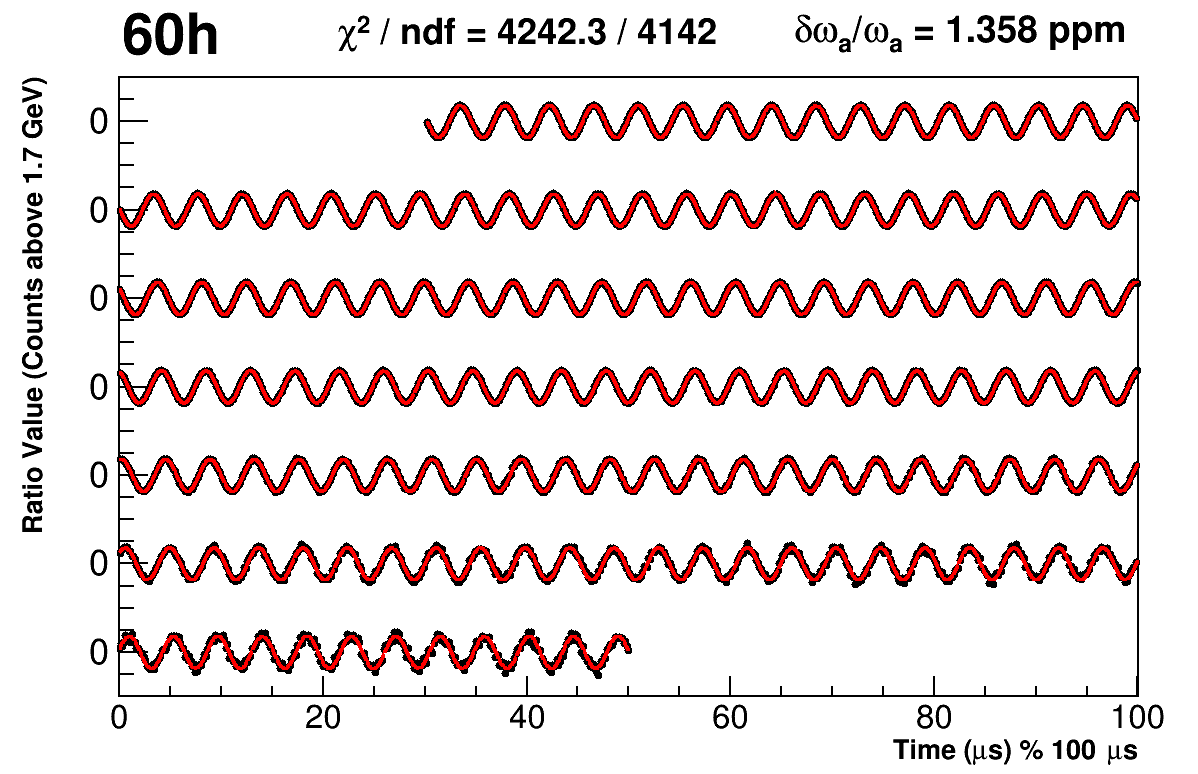
\includegraphics[width=\textwidth]{fullRatio_moduloPlot_noStats_60h}
        % \caption{60h dataset.}
    \end{subfigure}% %you need this % here to add spacing between subfigures
    \begin{subfigure}[]{0.45\textwidth}
        \centering
        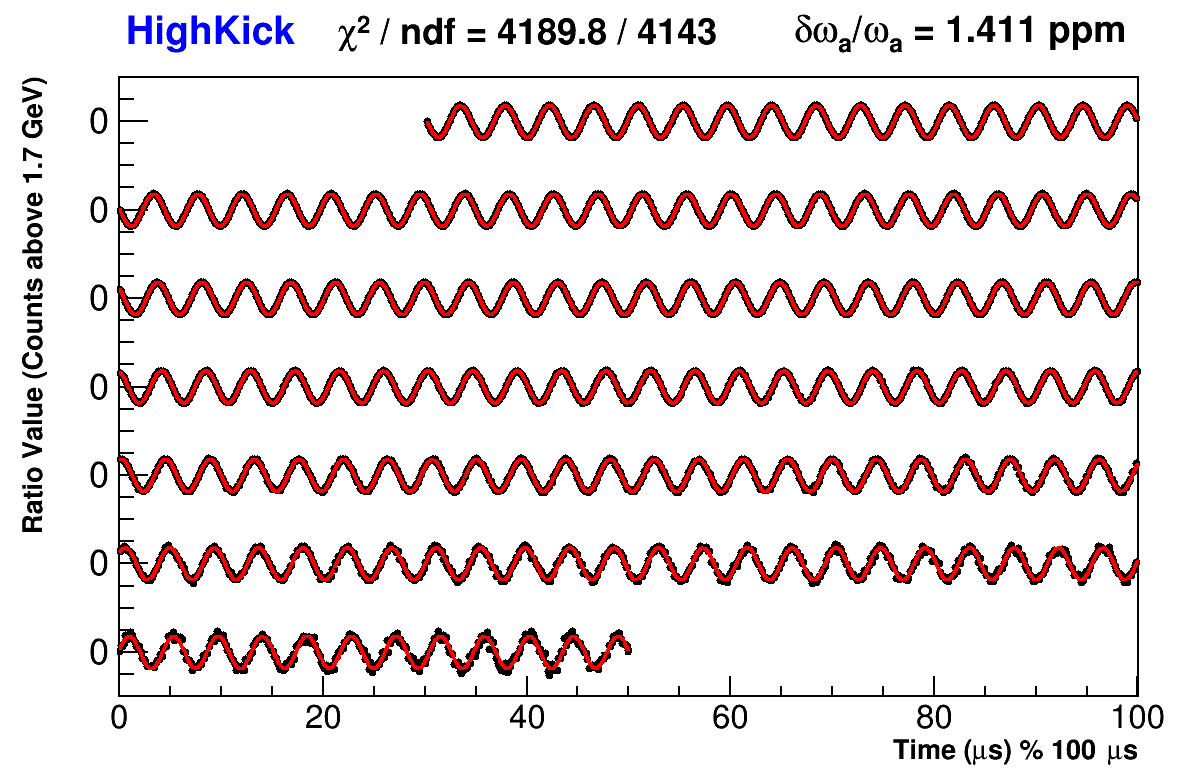
\includegraphics[width=\textwidth]{fullRatio_moduloPlot_noStats_HighKick}
        % \caption{HighKick dataset.}
    \end{subfigure}
    \vspace{4mm}
    \begin{subfigure}[]{0.45\textwidth}
        \centering
        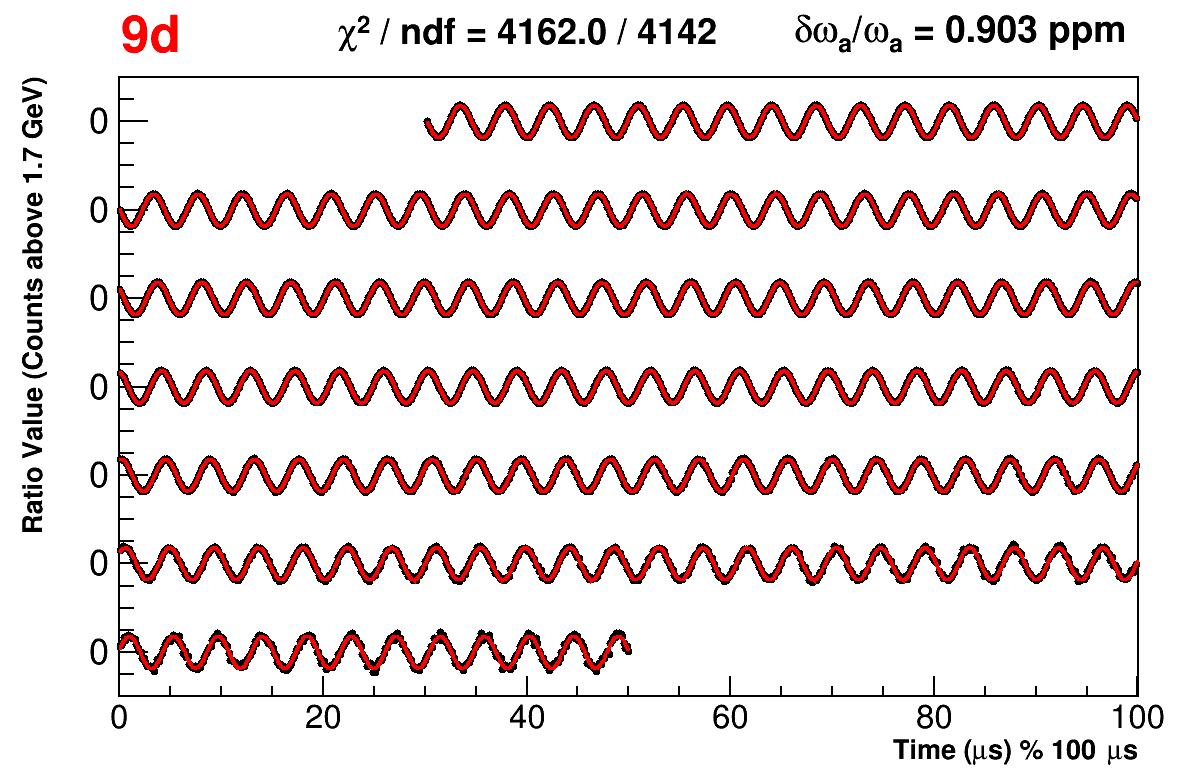
\includegraphics[width=\textwidth]{fullRatio_moduloPlot_noStats_9d}
        % \caption{9d dataset.}
    \end{subfigure}% %you need this % here to add spacing between subfigures
    \begin{subfigure}[]{0.45\textwidth}
        \centering
        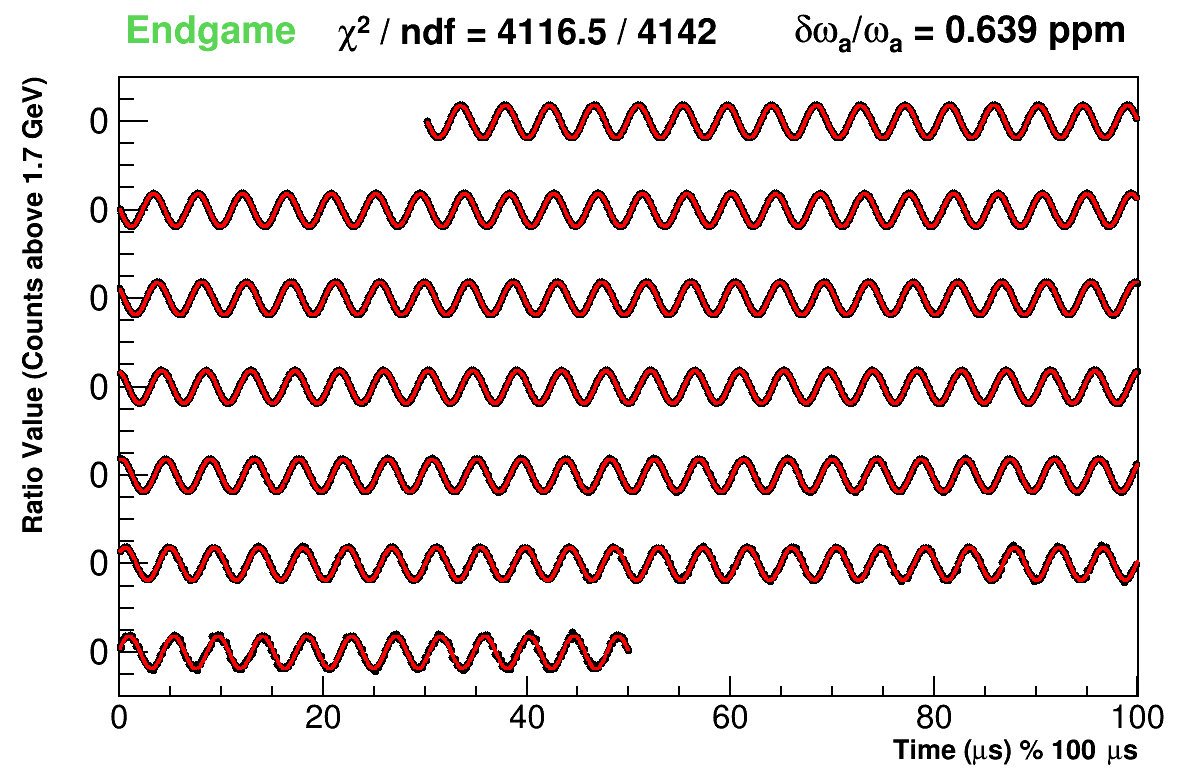
\includegraphics[width=\textwidth]{fullRatio_moduloPlot_noStats_Endgame}
        % \caption{Endgame dataset.}
    \end{subfigure}
\caption[Single random seed fits to calorimeter summed data of Run~1 precession frequency analysis datasets]{Single random seed fits to calorimeter summed data of Run~1 precession frequency analysis datasets. Data is in black and the fits are in red. The x axis is in units of \mus{} modulo \mus{100}, with successive portions of the data points and fit shifted downwards on the plot. The fit ranges from 30.2--\mus{650}. Dataset names are given in the upper left corners of the figures, alongside the \chisq per degree of freedom and relative error on \wa or $R$.}
\label{fig:moduloPlots}
\end{figure}



% \afterpage{
\clearrow
\begin{landscape}
\begin{table}
\centering
\small
% \setlength\tabcolsep{10pt}
\renewcommand{\arraystretch}{1.2}
% \begin{tabular*}{\linewidth}{@{\extracolsep{\fill}}l|cc|cc|cc|cc}
% \begin{tabular*}{\linewidth}{@{\extracolsep{\fill}}l|>{\rowmac}c>{\rowmac}c|>{\rowmac}c>{\rowmac}c|>{\rowmac}c>{\rowmac}c|>{\rowmac}c>{\rowmac}c<{\clearrow}}
\begin{tabular*}{\linewidth}{@{\extracolsep{\fill}}l|>{\rowmac}l>{\rowmac}l|>{\rowmac}l>{\rowmac}l|>{\rowmac}l>{\rowmac}l|>{\rowmac}l>{\rowmac}l<{\clearrow}}
% \begin{tabular*}{\linewidth}{@{\extracolsep{\fill}}l|>{\rowmac}S[table-format=3.3]>{\rowmac}S[table-format=3.3]|>{\rowmac}S[table-format=3.3]>{\rowmac}S[table-format=3.3]|>{\rowmac}S[table-format=3.3]>{\rowmac}S[table-format=3.3]|>{\rowmac}S[table-format=3.3]>{\rowmac}S[table-format=3.3]<{\clearrow}}
  \hline
    \multicolumn{9}{c}{\textbf{Ratio Method Fit Results}} \\
  \hline\hline
 & \multicolumn{2}{c|}{60h} & \multicolumn{2}{c|}{HighKick} & \multicolumn{2}{c|}{9d} & \multicolumn{2}{c}{Endgame} \\
  \hline\hline
    $\chi^{2}$/NDF & \multicolumn{2}{c|}{$4242/4142$} & \multicolumn{2}{c|}{$4190/4143$} & \multicolumn{2}{c|}{$4162/4142$} & \multicolumn{2}{c}{$4116/4142$} \\
    p-value        & \multicolumn{2}{c|}{$0.1356$} & \multicolumn{2}{c|}{$0.3018$} & \multicolumn{2}{c|}{$0.4104$} & \multicolumn{2}{c}{$0.6079$}  \\
  \hline\hline
    Parameter & Value & Error & Value & Error & Value & Error & Value & Error \\
  \hline
    $A$                               &  $\SI{0.3637}{}$ & $\SI{4.4e-05}{}$ & $\SI{0.3632}{}$ & $\SI{4.6e-05}{}$ & $\SI{0.3639}{}$ & $\SI{2.9e-05}{}$ & $\SI{0.3686}{}$ & $\SI{2.1e-05}{}$ \\
    
    \setrow{\bfseries} 
    $R$ (ppm, blinded)                &  $\SI{-20.8479}{}$ & $\SI{1.3581}{}$ & $\SI{-17.5433}{}$ & $\SI{1.4112}{}$ & $\SI{-17.8214}{}$ & $\SI{0.9033}{}$ & $\SI{-17.5674}{}$ & $\SI{0.6393}{}$ \\
    
    $\phi$                            &  $\SI{2.091}{}$ & $\SI{2.2e-4}{}$ & $\SI{2.081}{}$ & $\SI{2.3e-4}{}$ & $\SI{2.080}{}$ & $\SI{1.5e-4}{}$ & $\SI{2.076}{}$ & $\SI{1.1e-4}{}$ \\
    
    $\omega_{cbo}$ (rad/\mus{})       &  $\SI{2.338}{}$ & $\SI{1.4e-3}{}$ & $\SI{2.599}{}$ & $\SI{6.6e-3}{}$ & $\SI{2.615}{}$ & $\SI{5.6e-3}{}$ & $\SI{2.339}{}$ & $\SI{0.8e-3}{}$ \\
    
    $\tau_{cbo}$ (\mus{})             &  $\SI{175.2}{}$ & $\SI{46.8}{}$ & $\SI{99.4}{}$ & $\SI{0}{}$ & $\SI{137.4}{}$ & $\SI{62.0}{}$ & $\SI{200.3}{}$ & $\SI{33.5}{}$ \\
    
    $A_{cbo-N} \;(\times 10^{-4})$    &  $\SI{43.1}{}$ & $\SI{5.0}{}$ & $\SI{42.8}{}$ & $\SI{9.9}{}$ & $\SI{39.3}{}$ & $\SI{9.7}{}$ & $\SI{32.3}{}$ & $\SI{2.0}{}$ \\
    
    $\phi_{cbo-N}$                    &  $\SI{-2.343}{}$ & $\SI{0.107}{}$ & $\SI{3.817}{}$ & $\SI{0.446}{}$ & $\SI{3.302}{}$ & $\SI{0.374}{}$ & $\SI{-0.710}{}$ & $\SI{0.062}{}$ \\
    
    $A_{2cbo-N} \;(\times 10^{-4})$   &  $\SI{1.9}{}$ & $\SI{1.3}{}$ & $\SI{4.9}{}$ & $\SI{4.5}{}$ & $\SI{2.2}{}$ & $\SI{2.7}{}$ & $\SI{1.2}{}$ & $\SI{0.5}{}$ \\
    
    $\phi_{2cbo-N}$                   &  $\SI{3.331}{}$ & $\SI{0.638}{}$ & $\SI{5.665}{}$ & $\SI{1.274}{}$ & $\SI{-4.936}{}$ & $\SI{1.127}{}$ & $\SI{0.322}{}$ & $\SI{0.448}{}$ \\
   
    $A_{cbo-A} \;(\times 10^{-4})$    &  $\SI{05.5}{}$ & $\SI{3.9}{}$ & $\SI{9.5}{}$ & $\SI{4.1}{}$ & $\SI{6.4}{}$ & $\SI{2.5}{}$ & $\SI{2.7}{}$ & $\SI{1.9}{}$ \\
   
    $\phi_{cbo-A}$                    &  $\SI{-0.271}{}$ & $\SI{0.737}{}$ & $\SI{-2.073}{}$ & $\SI{0.600}{}$ & $\SI{1.750}{}$ & $\SI{0.561}{}$ & $\SI{-2.825}{}$ & $\SI{0.686}{}$ \\
    
    $A_{cbo-\phi} \;(\times 10^{-4})$ &  $\SI{8.0}{}$ & $\SI{4.2}{}$ & $\SI{5.7}{}$ & $\SI{4.4}{}$ & $\SI{8.8}{}$ & $\SI{3.1}{}$ & $\SI{1.9}{}$ & $\SI{1.9}{}$ \\
    
    $\phi_{cbo-\phi}$                 &  $\SI{-1.183}{}$ & $\SI{0.533}{}$ & $\SI{1.227}{}$ & $\SI{0.920}{}$ & $\SI{4.313}{}$ & $\SI{0.415}{}$ & $\SI{-1.576}{}$ & $\SI{0.995}{}$ \\
    
    $\kappa_{loss}$                   &  $\SI{8.974}{}$ & $\SI{0}{}$ & $\SI{5.651}{}$ & $\SI{0}{}$ & $\SI{2.510}{}$ & $\SI{0}{}$ & $\SI{2.345}{}$ & $\SI{0}{}$ \\
  \hline
\end{tabular*}
\caption[Fit results for Run~1 precession frequency analysis datasets]{Fit parameters for the four Run~1 precession frequency analysis datasets for a single random seed. The bold row highlights the final fitted $R$ values and their respective errors. The 60h dataset has a different blinding to the rest. The \K parameter is fixed in each dataset fit corresponding to the 0 value in the error column, and similarly for $\tau_{cbo}$ in the fit to the HighKick dataset.}
\label{tab:DatasetFitResults}
\end{table}
\end{landscape}
% }



% \afterpage{
\begin{landscape}
\begin{figure}
\centering
    \begin{subfigure}[b]{0.45\textwidth}
        \centering
        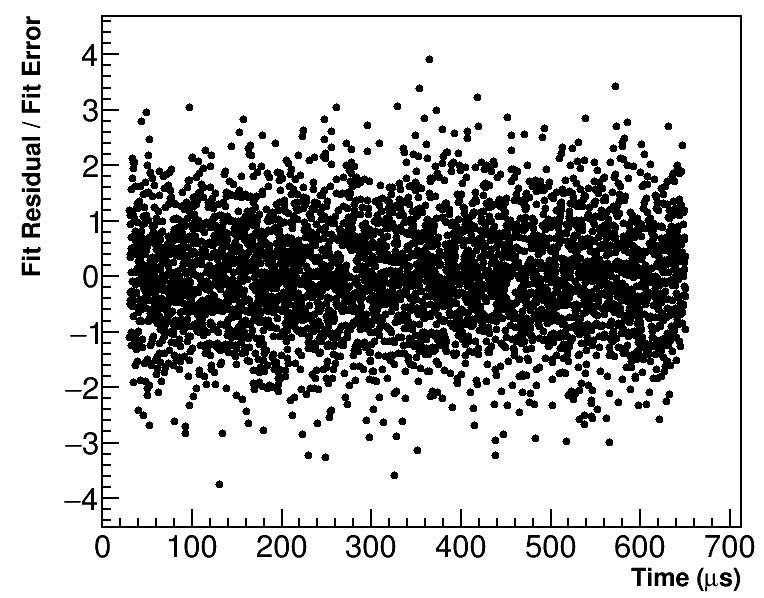
\includegraphics[width=\textwidth]{fitPull_60h}
    \vspace{4mm}
        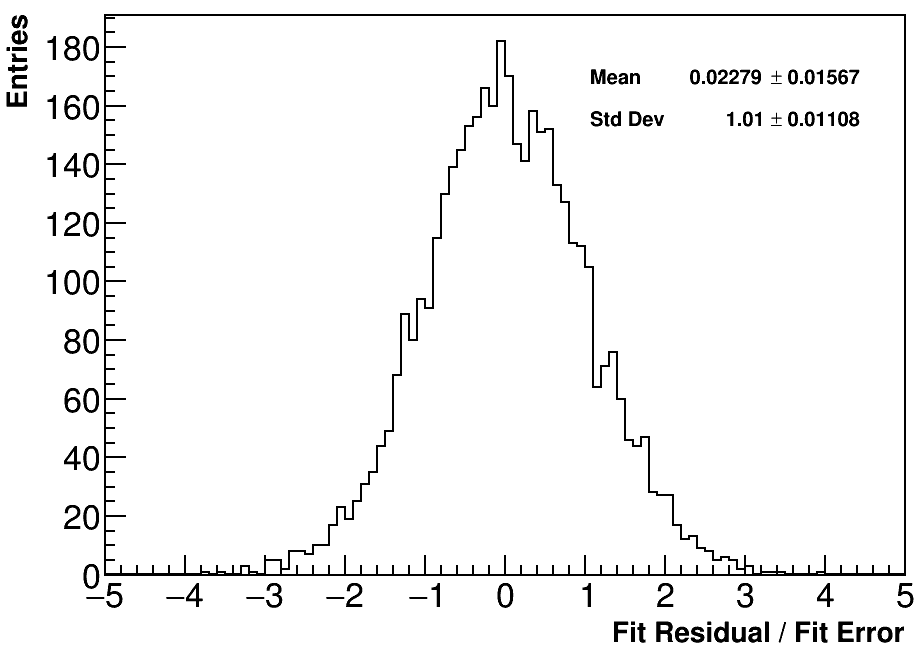
\includegraphics[width=\textwidth]{fitPull_projected_60h}
        % \caption{}
    \end{subfigure}
    % \hspace{5mm}
    \begin{subfigure}[b]{0.9\textwidth}
        \centering
        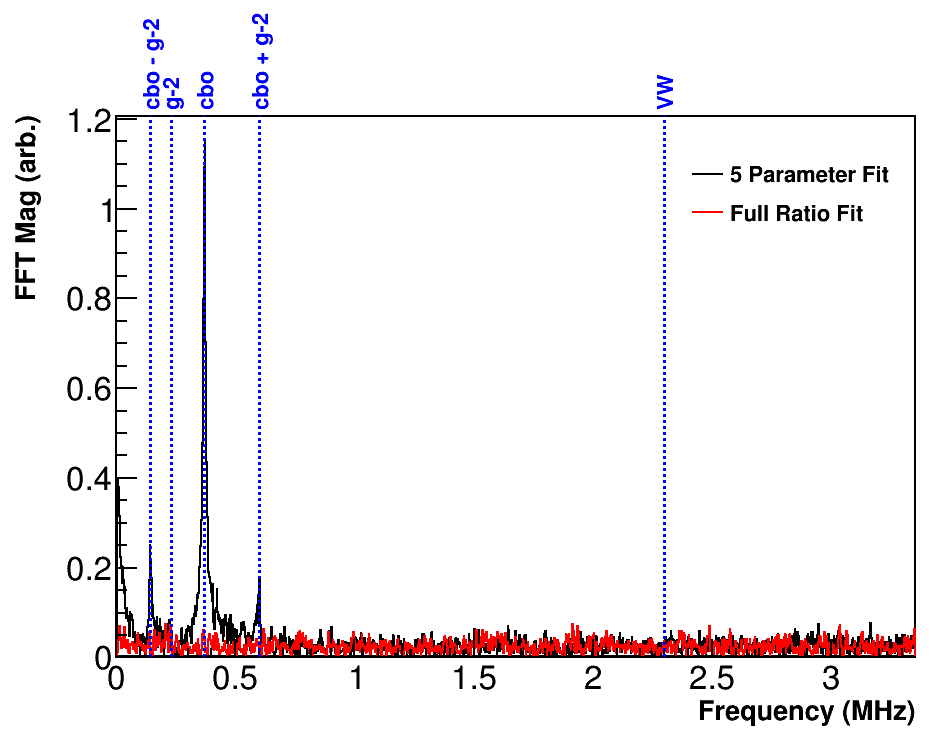
\includegraphics[width=\textwidth]{FFTComparison_FullRatio_60h}
        % \caption{}
        \vspace{1mm}
    \end{subfigure}
\caption[Pulls and FFT of residuals for the ratio fit to the 60h dataset]{Fit pulls (top-left), their projection onto the y-axis (bottom-left), and the FFT of the fit residuals (right) for the ratio fit to the 60h dataset. Note the pull projection has a Gaussian shape centered around zero with unit width. In the FFT the results from a five parameter fit to the data are overlayed, along with blue dashed lines for the main beam dynamics peaks which appear in the data. There is no obvious structure in the pulls and no remaining peaks above the noise in the ratio fit FFT.}
\label{fig:fitResiduals_60h}
\end{figure}
\end{landscape}
% }


The CBO frequencies for the 60h and Endgame datasets with $n$ values of 0.108 were found to be 2.338 and 2.339 rad/\mus{} respectively, corresponding to approximately \SI{0.37}{MHz}. For the HighKick and 9d datasets with $n$ values of 0.120, the CBO frequencies were found to be 2.559 and 2.615 rad/\mus{} respectively, corresponding to approximately \SI{0.415}{MHz}. These frequencies correspond to the expected frequencies as described in \secref{sec:muonbeamdynamics}, with some slight deviations due to statistics, bad resistors, and the reduced sensitivity in the Ratio Method\footnote{The VW frequencies, though time-randomized out in the analysis presented here, were found to be approximately \SI{2.30}{} and \SI{2.04}{MHz} for the datasets with $n=0.108$ and $n=0.120$ respectively.}. The CBO lifetimes between the different datasets are relatively consistent, barring the HighKick dataset for which a smaller CBO lifetime was measured, attributed to the changing behavior of the bad resistors in that dataset. Ratio Method fits typically converge with lifetimes with large errors compared to T-Method fits, due to the reduction in sensitivity in the Ratio Method. In the HighKick dataset, the CBO lifetime did not like to converge nicely in the ratio fits, and was therefore fixed to that from a T-Method fit. The main CBO amplitudes $A_{cbo-N}$ for the different datasets were on the order of 0.3--0.4\%, while the higher order CBO amplitudes were in general an order of magnitude less. The strength of the various higher order CBO amplitudes fluctuated for different datasets, with one parameter being large compared to another in one dataset and vice versa in a different dataset. In some cases, the errors on the higher order CBO term amplitudes were of the order the amplitude itself. While this implies these terms can be dropped from the fit function, all terms were included for analysis uniformity among the different datasets. These relatively large errors, while making some of the fits slightly more challenging to achieve convergence, were nonetheless handled appropriately.



The final statistical errors on $R$ for the 60h, HighKick, 9d, and Endgame datasets are \SI{1.358}{}, \SI{1.411}{}, \SI{0.903}{}, and \SI{0.639}{ppm} respectively. The single seed $R$ results for the HighKick, 9d, and Endgame datasets, all of which used the same blinding string, are all well within $1\sigma$ of each other. The average $R$ value for fits to 50 different random seeds are provided in \secref{sub:randomSeedFits}.


Beyond looking at single fit residuals to evaluate the integrity of the fits, other checks were made to verify consistency. In general this consisted of slicing up the data in different ways and fitting the subsets. These tests and scans included fitting individual calorimeters, modifying the fit start and end times, adjusting the applied energy thresholds, and fitting individual beam bunches.





% \clearpage

\subsection{Individual calorimeter fits}
\label{sub:per_calorimeter_fits}


Fits to all 24 individual calorimeters for each of the datasets were performed with the same number of free fit parameters as used in the calorimeter sum fits. \figref{fig:caloFits_chi2} shows the \chisq/NDF's for the calorimeter fits which are nicely spread around 1. \figref{fig:caloFits_R} shows the fitted $R$ values as a function of calorimeter number. Straight line fits were performed to the $R$ values with good \chisq's, and the fitted constant returned a value in each case that was consistent with the calorimeter sum fit $R$ values. Examining the $R$ values as a function of calorimeter between datasets, particular calorimeter numbers do not tend to lie above or below the fitted average. The spread in $R$ values for each calorimeter then can be said to be driven statistically, though it should be noted that with the larger error bars on the individual calorimeter fits it's hard to tell if there are any preferences one way or another.


\begin{figure}
\centering
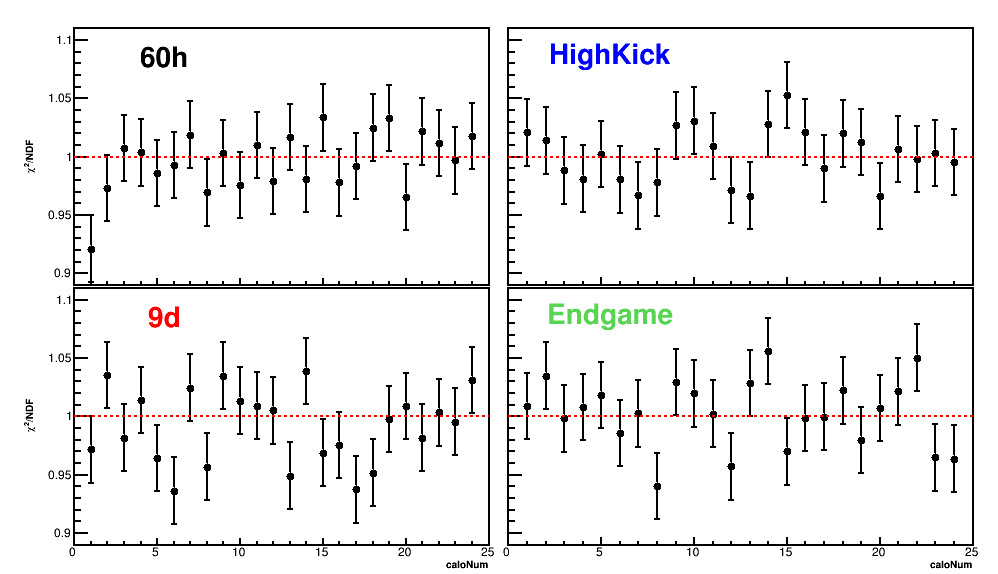
\includegraphics[width=0.84\linewidth]{caloFits_chi2_fourDatsets}
    \caption[\chisq/NDF versus calorimeter number]{\chisq/NDF versus calorimeter for the Run~1 precession frequency analysis datasets. Red dashed lines are placed at $\chi^{2}/\text{NDF} = 1$ to aid the eye. No individual calorimeter fits are preferentially low or high when comparing across datasets.}
    \label{fig:caloFits_chi2}
\vspace{4mm}
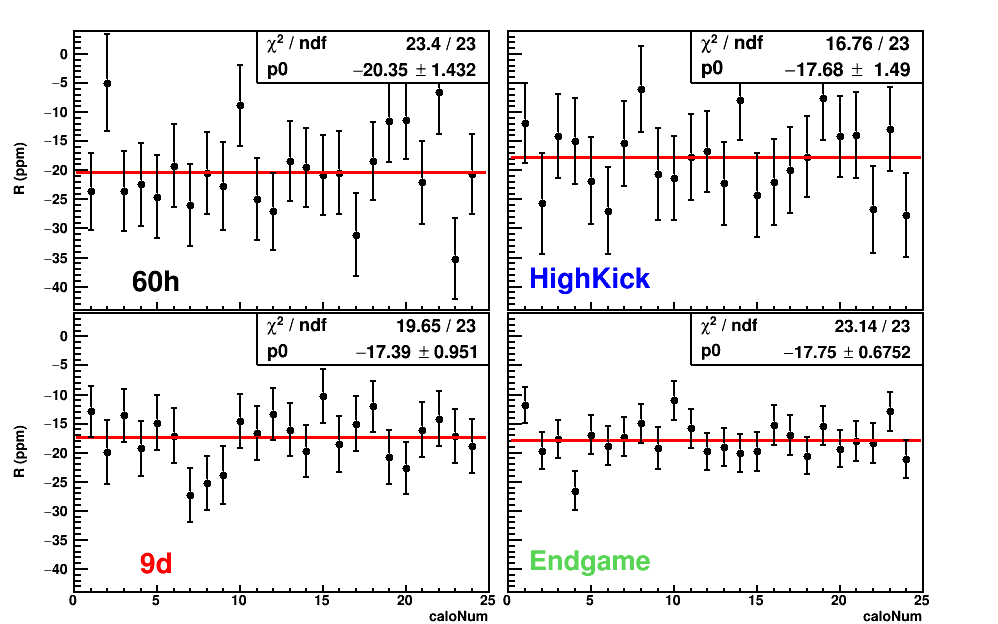
\includegraphics[width=0.84\linewidth]{caloFits_R_fourDatsets}
    \caption[$R$ versus calorimeter number]{$R$ versus calorimeter for the Run~1 precession frequency analysis datasets. The scale is the same on each of the plots.  A straight line fit was performed on the fitted values, with the fit result shown in the upper right box as parameter $p_{1}$ in units of ppm.The different blinding in the 60h dataset is readily observed, along with the higher precision fits in the 9d and Endgame datasets with their correspondingly smaller error bars.}
    \label{fig:caloFits_R}
\end{figure}


Figures~\ref{fig:caloFits_EndgamePars_1} and \ref{fig:fig:caloFits_EndgamePars_2} show calorimeter fit results for the other free parameters in the fit for the Endgame dataset. The \gmtwo phases are seen to be distinct among the different calorimeters, attributed to the different level of material upstream and therefore different acceptance. This is particularly noticeable in calorimeters 13 and 19 which sit behind the tracker stations. Any correlated effects on $R$ are not immediately observed, and might potentially be hidden behind the large errors of the fit. Similarly, the different calorimeters have different fit asymmetries, once again due to their different acceptances. The CBO parameters are in general consistent with some spread due to acceptance, with the phases running from 0--2$\pi$ around the ring as expected. The amplitudes of the CBO parameters are an order of magnitude higher than in the calorimeter sum fits. Because the phases vary around the ring, when adding up all the calorimeters the CBO effect becomes reduced. In fact, while it is not always necessary to include the higher order CBO terms for good fits to the calorimeter sum data, there are many calorimeters which need the higher order terms for good fits.


\begin{figure}
\centering
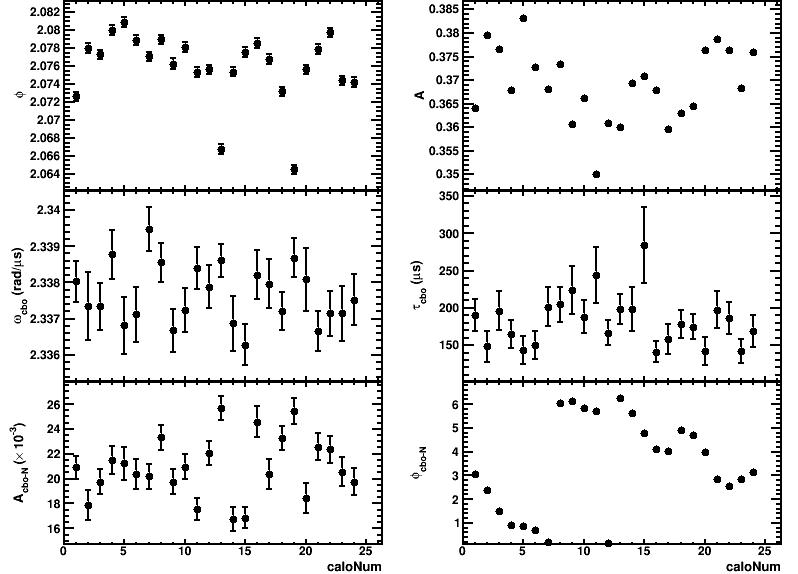
\includegraphics[width=.9\textwidth]{Endgame_caloFitPars_first}
\caption[Endgame fit parameters versus calorimeter number]{Endgame fit parameters versus calorimeter number. In the  \gmtwo phase $\phi$ (top-left) two points lie below the others, corresponding to those calorimeters which sit behind tracker stations. The CBO phase $\phi_{cbo-N}$ (bottom-right) runs from 0--2$\pi$ around the ring. These plots are typical of all datasets, with small variations in the final fitted parameters.}
\label{fig:caloFits_EndgamePars_1}
\end{figure}


\begin{figure}[t]
\centering
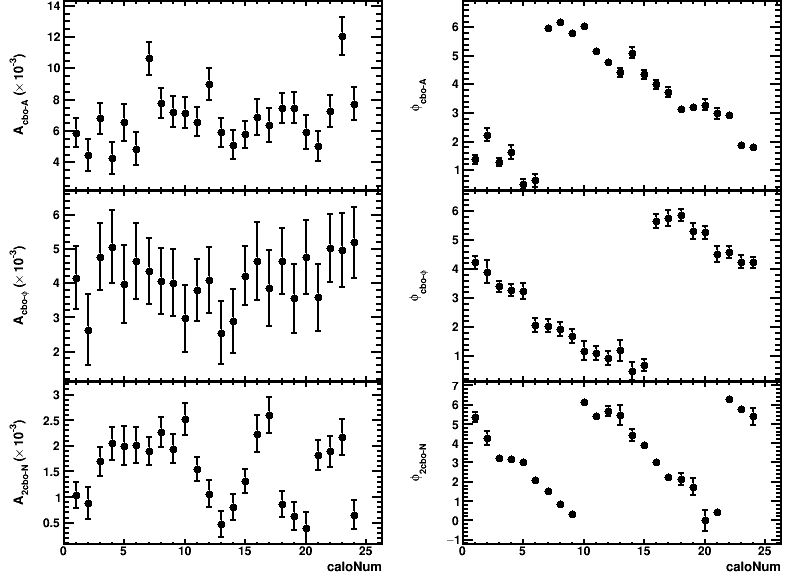
\includegraphics[width=.9\textwidth]{Endgame_caloFitPars_second}
\caption[Additional Endgame fit parameters versus calorimeter number]{Additional Endgame fit parameters versus calorimeter number. The CBO phases $\phi_{cbo-A}$ and $\phi_{cbo-\phi}$ run from 0--2$\pi$ around the ring, while $\phi_{2cbo-N}$ runs around twice. These plots are typical of all datasets, with small variations in the final fitted parameters.}
\label{fig:fig:caloFits_EndgamePars_2}
\end{figure}


% \begin{figure}
% \centering
%     \begin{subfigure}[]{0.45\textwidth}
%         \centering
%         \includegraphics[width=\textwidth]{FullRatioFit_phi_Vs_Calo_Canv_Endgame}
%         \caption{$\phi$}
%     \end{subfigure}% %you need this % here to add spacing between subfigures
%     \begin{subfigure}[]{0.45\textwidth}
%         \centering
%         \includegraphics[width=\textwidth]{FullRatioFit_A_Vs_Calo_Canv_Endgame}
%         \caption{$A$}
%     \end{subfigure}

%     \begin{subfigure}[]{0.45\textwidth}
%         \centering
%         \includegraphics[width=\textwidth]{FullRatioFit_omega_cbo_Vs_Calo_Canv_Endgame}
%         \caption{$\omega_{cbo}$}
%     \end{subfigure}% %you need this % here to add spacing between subfigures
%     \begin{subfigure}[]{0.45\textwidth}
%         \centering
%         \includegraphics[width=\textwidth]{FullRatioFit_tau_cbo_Vs_Calo_Canv_Endgame}
%         \caption{$\tau_{cbo}$}
%     \end{subfigure}

%     \begin{subfigure}[]{0.45\textwidth}
%         \centering
%         \includegraphics[width=\textwidth]{FullRatioFit_A_cbo-N_Vs_Calo_Canv_Endgame}
%         \caption{$A_{cbo-N}$}
%     \end{subfigure}% %you need this % here to add spacing between subfigures
%     \begin{subfigure}[]{0.45\textwidth}
%         \centering
%         \includegraphics[width=\textwidth]{FullRatioFit_phi_cbo-N_Vs_Calo_Canv_Endgame}
%         \caption{$\phi_{cbo-N}$}
%     \end{subfigure}
% \caption[Endgame fit parameters versus calorimeter number]{Endgame fit parameters versus calorimeter number. In the  \gmtwo phase $\phi$ (top-left) two points lie below the others, corresponding to those calorimeters which sit behind tracker stations. The CBO phase $\phi_{cbo-N}$ (bottom-right) runs from 0--2$\pi$ around the ring. These plots are typical of all datasets, with small variations in the final fitted parameters.}
% \label{fig:caloFits_EndgamePars_1}
% \end{figure}

% \begin{figure}
% \centering
%     \begin{subfigure}[]{0.45\textwidth}
%         \centering
%         \includegraphics[width=\textwidth]{FullRatioFit_A_cbo-A_Vs_Calo_Canv_Endgame}
%         \caption{$A_{cbo-A}$}
%     \end{subfigure}% %you need this % here to add spacing between subfigures
%     \begin{subfigure}[]{0.45\textwidth}
%         \centering
%         \includegraphics[width=\textwidth]{FullRatioFit_phi_cbo-A_Vs_Calo_Canv_Endgame}
%         \caption{$\phi_{cbo-A}$}
%     \end{subfigure}

%     \begin{subfigure}[]{0.45\textwidth}
%         \centering
%         \includegraphics[width=\textwidth]{FullRatioFit_A_cbo-phi_Vs_Calo_Canv_Endgame}
%         \caption{$A_{cbo-\phi}$}
%     \end{subfigure}% %you need this % here to add spacing between subfigures
%     \begin{subfigure}[]{0.45\textwidth}
%         \centering
%         \includegraphics[width=\textwidth]{FullRatioFit_phi_cbo-phi_Vs_Calo_Canv_Endgame}
%         \caption{$\phi_{cbo-\phi}$}
%     \end{subfigure}

%     \begin{subfigure}[]{0.45\textwidth}
%         \centering
%         \includegraphics[width=\textwidth]{FullRatioFit_A_2cbo-N_Vs_Calo_Canv_Endgame}
%         \caption{$A_{2cbo-N}$}
%     \end{subfigure}% %you need this % here to add spacing between subfigures
%     \begin{subfigure}[]{0.45\textwidth}
%         \centering
%         \includegraphics[width=\textwidth]{FullRatioFit_phi_2cbo-N_Vs_Calo_Canv_Endgame}
%         \caption{$\phi_{2cbo-N}$}
%     \end{subfigure}
% \caption[Additional Endgame fit parameters versus calorimeter number]{Additional Endgame fit parameters versus calorimeter number. The CBO phases $\phi_{cbo-A}$ and $\phi_{cbo-\phi}$ run from 0--2$\pi$ around the ring, while $\phi_{2cbo-N}$ runs around twice. These plots are typical of all datasets, with small variations in the final fitted parameters.}
% \label{fig:fig:caloFits_EndgamePars_2}
% \end{figure}


% \clearpage

\subsection{Scans over fit start time, fit end time, and energy threshold}


In order to determine if there are any deficiencies as a function of time, for instance if the CBO was modeled incorrectly, fits are performed with varying fit start and end times. If a parameter is incorrectly modeled, it will wander away from the statistically allowed deviation as the mis-modeled effect grows stronger or weaker. Two examples of this are given in \figref{fig:badStartScans}. In the first case the CBO frequency was mis-measured when excluding the changing CBO frequency model, and in the second case the asymmetry was mis-measured when pileup was not subtracted from the data. In general, doing a fit start scan is a very useful tool in the precession frequency analysis beyond just verifying consistency of a fit parameter as a function of time, as it also provides hints as to what might be wrong with how the data is being handled.


\begin{figure}[h]
\centering
    \begin{subfigure}[t]{0.45\textwidth}
        \centering
        \includegraphics[width=\textwidth]{FullRatio_omega_cbo_FS_Canv_Endgame_fixedCBOModel}
        \caption{The fit start scan for the fitted CBO frequency when a constant frequency model is included. The p-value of the first ratio fit in this case is 0.191, indicating an acceptable fit. Only by performing a fit start scan or examining the fit residuals closely is the deficiency in the fit observed.}
    \end{subfigure}% %you need this % here to add spacing between subfigures
    \hspace{4mm}
    \begin{subfigure}[t]{0.45\textwidth}
        \centering
        \includegraphics[width=\textwidth]{FullRatio_A_FS_Canv_Endgame_noPileupSubraction}
        \caption{The fit start scan for the fitted asymmetry when the pileup is not subtracted out. If the pileup is not properly accounted for, then decay positrons with lower asymmetries contaminate the observed decay time spectrum leading to a lower fitted asymmetry value. As the pileup diminishes the fitted asymmetry tends to it's true value.}
    \end{subfigure}
\caption[Examples of fit start scans when effects are improperly accounted for before or during fitting]{Examples of fit start scans when effects are improperly accounted for before or during fitting. The parabolic bands indicate the one sigma allowed deviation in the fit parameters due to the changing statistics between the fits. Data are from the Endgame dataset.}
\label{fig:badStartScans}
\end{figure}



The statistically allowed deviation between two sets of \gmtwo data, where one is a subset of the other, is given by~\cite{E821FinalReport}
  \begin{align} \label{eq:sigmaDiffFull}
    \sigma_{diff} = \sqrt{\sigma_{2} - \sigma_{1}(2 \frac{A_{1}}{A_{2}}\cos(\phi_{1}-\phi_{2}) - 1)},
  \end{align}
where the subscript 2 stands for the larger dataset while the subscript 1 stands for the smaller sub-dataset. This statistically allowed deviation depends both on the size of the datasets as well as their ``analyzing powers,'' which come from the asymmetries and phases of the datasets. For fit start scans the analyzing powers are in general the same, such that the approximation 
  \begin{align} \label{eq:sigmaDiffApprox}
    \sigma_{diff} \approx \sqrt{\sigma_{2} - \sigma_{1}}
  \end{align}
can be made. 


It should be noted that for fits with late fit start times, certain CBO parameters start to become unstable as the CBO effect becomes diminished in the data\footnote{The same applies to the VW effect when it is not time-randomized out of the data.}. Fits with start times at \mus{100} are half a lifetime or more along the CBO effect and convergence is difficult to achieve. For those parameters which were found to be unreliable, they were fixed to their starting fit values. These typically included the CBO lifetime and most of the higher order CBO amplitudes and phases, though in some cases they could still be included out to late fit start times depending on the dataset.


Fit start time scans were performed from the default value of \mus{30.2} up to \mus{100.2} in steps of \mus{1} corresponding to 71 separate fits. In order to assist fit convergence, the final fit parameters from one fit were passed on as the starting parameters of the next. The \chisq/NDF's and fitted $R$ values as a function of fit start time for the four Run~1 precession frequency analysis datasets are shown in \figref{fig:fitStartTime_chi2_and_R}. The error on the individual points in the \chisq plots are given as 
  \begin{align}
    \sigma_{\chi^{2}/NDF} = \sqrt{2/NDF},
  \end{align}
where NDF changes as the fit start time is pushed later in time and bins are left out of the fit. The black parabolic bands indicate the $1\sigma$ statistically allowed deviation as given by \equref{eq:sigmaDiffApprox}. As shown the goodness of fit for the four datasets are all consistent with fit start time, only wandering in and near the bands without diverging.


\begin{landscape}
\begin{figure}
    \centering
    \includegraphics[width=1\linewidth]{fitStartScan_R_fourDatasets}
    \caption[\chisq/NDF and $R$ versus fit start time]{\chisq/NDF (top) and $R$ (bottom) versus fit start time for the Run~1 precession frequency analysis datasets. Plots in the top and bottom rows are on the same scale respectively. The black parabolic bands represent the $1\sigma$ statistically allowed deviation. The \chisq values are all consistent with 1, for which a dashed red line has been overlayed. In all cases the fit points lie in and around the $1\sigma$ statistical bands.}
    \label{fig:fitStartTime_chi2_and_R}
\end{figure}
\end{landscape}


$R$ is similarly consistent as a function of fit start time. The only dataset for which $R$ goes noticeably outside the bands more than the others is that for the HighKick. Since the deviation is less than $2\sigma$ and it appears to have a trend back towards the bands however, it does not appear particularly indicative of unaccounted effects in the data. In general $R$ is very insensitive to changing fit start time, most likely due to the small correlations with other fit parameters.


\figref{fig:fitStartScan_EndgamePars} shows the fit start scan results for the other free parameters for the Endgame dataset. In all cases the fit parameters only wander in and near the bands, showing that all effects in the ratio data are properly accounted for.


\begin{figure}[h]
\centering
\includegraphics[width=.9\textwidth]{Endgame_fitStartScan_pars}
\caption[Fit start scans for free parameters in the Endgame dataset]{Fit start scans for free parameters in the Endgame dataset. Those parameters not shown here are fixed to their starting values over the course of the scan, as at late times they can be unstable as the CBO effects die away.}
\label{fig:fitStartScan_EndgamePars}
\end{figure}


% \begin{figure}
% \centering
%     \begin{subfigure}[]{0.45\textwidth}
%         \centering
%         \includegraphics[width=\textwidth]{FullRatio_phi_FS_Canv_Endgame}
%         \caption{$\phi$}
%     \end{subfigure}% %you need this % here to add spacing between subfigures
%     \begin{subfigure}[]{0.45\textwidth}
%         \centering
%         \includegraphics[width=\textwidth]{FullRatio_A_FS_Canv_Endgame}
%         \caption{$A$}
%     \end{subfigure}

%     \begin{subfigure}[]{0.45\textwidth}
%         \centering
%         \includegraphics[width=\textwidth]{FullRatio_omega_cbo_FS_Canv_Endgame}
%         \caption{$\omega_{cbo}$}
%     \end{subfigure}% %you need this % here to add spacing between subfigures
%     \begin{subfigure}[]{0.45\textwidth}
%         \centering
%         \includegraphics[width=\textwidth]{FullRatio_phi_cbo-N_FS_Canv_Endgame}
%         \caption{$\phi_{cbo-N}$}
%     \end{subfigure}

%     \begin{subfigure}[]{0.45\textwidth}
%         \centering
%         \includegraphics[width=\textwidth]{FullRatio_A_cbo-N_FS_Canv_Endgame}
%         \caption{$A_{cbo-N}$}
%     \end{subfigure}% %you need this % here to add spacing between subfigures
%     \begin{subfigure}[]{0.45\textwidth}
%         \centering
%         \includegraphics[width=\textwidth]{FullRatio_A_cbo-phi_FS_Canv_Endgame}
%         \caption{$A_{cbo-\phi}$}
%     \end{subfigure}
% \caption[Fit start scans for free parameters in the Endgame dataset]{Fit start scans for free parameters in the Endgame dataset. Those parameters not shown here are fixed to their starting values over the course of the scan, as at late times they can be unstable as the CBO effects die away.}
% \label{fig:fitStartScan_EndgamePars}
% \end{figure}


For fit end scans, all of the same methods and conclusions apply. In general fit end scans are both less dangerous and more stable than fit start scans, as the amount of data being removed from the fit is relatively small. While these fit end scans in a T-Method fit might be able to be completely ignored in favor of the fit start scans, it's important to check that they satisfy the statistical deviations in the Ratio Method as the ratio data errors grow larger with less data~\cite{BU60hReport}. Fit end time scans were performed from \mus{650} to \mus{400} in steps of \mus{10}, corresponding to 26 separate fits. As in the fit start time scan, fit results from the end of one fit were passed on as the starting parameters to the next. $R$ values for fit end scans for the Run~1 precession frequency analysis datasets are shown in \figref{fig:fitEndTime_R}. As shown the $R$ values are comfortably within and near the bands.


Similarly to fit start and end time scans, it is worthwhile to verify that $R$ is consistent regardless of the energy threshold applied to the decay positron time spectrum. The energy threshold was varied from \SI{1.2}{\GeV} to \SI{2.2}{\GeV} in steps of \SI{50}{\MeV} corresponding to 21 separate fits. The fitted $R$ values for the four Run~1 precession frequency analysis datasets are shown in \figref{fig:energyThresholdScan_R}. The statistical bands are the same as those defined in \equref{eq:sigmaDiffFull}, where now the analyzing power part of the equation plays a larger role as the asymmetries and phases of the different fit points are significantly different. As shown there are no major deviations in the fitted $R$ values.



\begin{figure}[H]
\centering
    \vspace{-4mm}
    \begin{subfigure}[]{0.35\textwidth}
        \centering
        \includegraphics[width=\textwidth]{FullRatio_R_FE_Canv_60h}
        \caption{60h dataset.}
    \end{subfigure}% %you need this % here to add spacing between subfigures
    \begin{subfigure}[]{0.35\textwidth}
        \centering
        \includegraphics[width=\textwidth]{FullRatio_R_FE_Canv_HighKick}
        \caption{HighKick dataset.}
    \end{subfigure}

    \begin{subfigure}[]{0.35\textwidth}
        \centering
        \includegraphics[width=\textwidth]{FullRatio_R_FE_Canv_9d}
        \caption{9d dataset.}
    \end{subfigure}% %you need this % here to add spacing between subfigures
    \begin{subfigure}[]{0.35\textwidth}
        \centering
        \includegraphics[width=\textwidth]{FullRatio_R_FE_Canv_Endgame}
        \caption{Endgame dataset.}
    \end{subfigure}
\caption[$R$ versus fit end time]{$R$ versus fit end time for the Run~1 precession frequency analysis datasets. The fit points lie in and around the $1\sigma$ statistical bands.}
\label{fig:fitEndTime_R}
\end{figure}


\begin{figure}[H]
\centering
    \vspace{-4mm}
    \begin{subfigure}[]{0.35\textwidth}
        \centering
        \includegraphics[width=\textwidth]{FullRatio_R_Vs_ETh_60h}
        \caption{60h dataset.}
    \end{subfigure}% %you need this % here to add spacing between subfigures
    \begin{subfigure}[]{0.35\textwidth}
        \centering
        \includegraphics[width=\textwidth]{FullRatio_R_Vs_ETh_HighKick}
        \caption{HighKick dataset.}
    \end{subfigure}

    \begin{subfigure}[]{0.35\textwidth}
        \centering
        \includegraphics[width=\textwidth]{FullRatio_R_Vs_ETh_9d}
        \caption{9d dataset.}
    \end{subfigure}% %you need this % here to add spacing between subfigures
    \begin{subfigure}[]{0.35\textwidth}
        \centering
        \includegraphics[width=\textwidth]{FullRatio_R_Vs_ETh_Endgame}
        \caption{Endgame dataset.}
    \end{subfigure}
\caption[$R$ versus energy threshold]{$R$ versus energy threshold for the Run~1 precession frequency analysis datasets. The fit points lie in and around the $1\sigma$ statistical bands.}
\label{fig:energyThresholdScan_R}
\end{figure}



% \clearpage


\subsection{Fits to bunch number}

Eight distinct and separate bunches of muons are sent to the E989 experiment within the accelerator timing structure as described in \secref{sec:Accelerator}. Differences upstream and at injection mean that the stored beam is slightly different between the bunches. In order to verify that the treatment of fit parameters was correct regardless of the bunch number and improve confidence in the results, the bunches were fit individually. \figref{fig:bunchNum_R} shows the fitted $R$ values for the eight individual bunches alongside the bunch-sum result, for the Run~1 precession frequency analysis datasets. In all cases there appear no systematically different $R$ values per bunch. When the eight individual bunches were fit to a straight line, they were found to be consistent with the bunch-sum result.


% If different bunches have different momentum spreads due to how the particles are transported down the various beamlines and injected into the storage ring, then muons might live for different times and therefore their spins might precess more or less within the magnetic field. This difference in \gmtwo phase between the different bunches would then affect the final fitted $R$ value, and might be a systematic error in the precession frequency measurement if certain bunches have significantly more statistics than the others. <- wrong


\begin{figure}
\centering
    \begin{subfigure}[]{0.45\textwidth}
        \centering
        \includegraphics[width=\textwidth]{FullRatio_R_Vs_BunchNum_Canv_60h}
        \caption{60h dataset.}
    \end{subfigure}% %you need this % here to add spacing between subfigures
    \begin{subfigure}[]{0.45\textwidth}
        \centering
        \includegraphics[width=\textwidth]{FullRatio_R_Vs_BunchNum_Canv_HighKick}
        \caption{HighKick dataset.}
    \end{subfigure}

    \begin{subfigure}[]{0.45\textwidth}
        \centering
        \includegraphics[width=\textwidth]{FullRatio_R_Vs_BunchNum_Canv_9d}
        \caption{9d dataset.}
    \end{subfigure}% %you need this % here to add spacing between subfigures
    \begin{subfigure}[]{0.45\textwidth}
        \centering
        \includegraphics[width=\textwidth]{FullRatio_R_Vs_BunchNum_Canv_Endgame}
        \caption{Endgame dataset.}
    \end{subfigure}
\caption[$R$ versus bunch number]{$R$ versus bunch number for the Run~1 precession frequency analysis datasets. Bunch number 0 corresponds to the data from all bunches added together. The blue dashed line intersects the bunch number 0 point, and it's value is displayed in the top left of each plot. The red line corresponds to a fit to bunches 1--8, with $p_{0}$ being the fit parameter. In all cases the fitted $R$ value to bunches 1--8 is nearly identical to the all-bunches result.}
\label{fig:bunchNum_R}
\end{figure}


\clearpage


\subsection{Fits to many random seeds}
\label{sub:randomSeedFits}


While the single seed fit results presented earlier indicate good fits and well understood parameters, it is always a good idea to fit other random seeds in case the single seed results ended up on an outlier. Doing so not only improves the confidence of the result, but also gives a more central $R$ value to quote as being closer to the `true' $R$ of the dataset. Figure~\ref{fig:randomSeedFits_chi2_and_R} gives the \chisq and $R$ distributions for fits to 50 different random seeds for the four datasets. As shown the \chisq distributions are centered around 1 as expected. \tabref{tab:RandomSeedFitResults} compares the random seed fit results between the different datasets. The means for the $R$ distributions of the datasets which shared the same blinding string (HighKick, 9d, Endgam) are statistically consistent with one another, with differences on the order of several hundreds of ppb, well within the statistical errors of \SI{600}{ppb} or greater\footnote{The errors on the mean are calculated as $\sigma_{\mu} = \text{RMS}/\sqrt{N},$ where $N$ is the number of random seeds. These errors come from the randomization of cluster times before fitting, and have no bearing on statistical consistency when comparing different datasets.}.

% \begin{figure}
% \centering
%     \begin{subfigure}[]{0.45\textwidth}
%         \centering
%         \includegraphics[width=\textwidth]{FullRatio_Chi2NDF_Vs_Iter_Canv_hist_60h}
%         \caption{60h dataset.}
%     \end{subfigure}% %you need this % here to add spacing between subfigures
%     \begin{subfigure}[]{0.45\textwidth}
%         \centering
%         \includegraphics[width=\textwidth]{FullRatio_Chi2NDF_Vs_Iter_Canv_hist_HighKick}
%         \caption{HighKick dataset.}
%     \end{subfigure}

%     \begin{subfigure}[]{0.45\textwidth}
%         \centering
%         \includegraphics[width=\textwidth]{FullRatio_Chi2NDF_Vs_Iter_Canv_hist_9d}
%         \caption{9d dataset.}
%     \end{subfigure}% %you need this % here to add spacing between subfigures
%     \begin{subfigure}[]{0.45\textwidth}
%         \centering
%         \includegraphics[width=\textwidth]{FullRatio_Chi2NDF_Vs_Iter_Canv_hist_Endgame}
%         \caption{Endgame dataset.}
%     \end{subfigure}
% \caption[\chisq's for fits to many random seeds]{\chisq values for fits to 50 different random seeds for the Run~1 precession frequency analysis datasets. The distributions are nicely centered around 1 which is to be expected if the randomized data is properly distributed and fit correctly.}
% \label{fig:randomSeedFits_chi2}
% \end{figure}


% \begin{figure}
% \centering
%     \begin{subfigure}[]{0.45\textwidth}
%         \centering
%         \includegraphics[width=\textwidth]{FullRatio_R_Vs_Iter_Canv_hist_60h}
%         \caption{60h dataset.}
%     \end{subfigure}% %you need this % here to add spacing between subfigures
%     \begin{subfigure}[]{0.45\textwidth}
%         \centering
%         \includegraphics[width=\textwidth]{FullRatio_R_Vs_Iter_Canv_hist_HighKick}
%         \caption{HighKick dataset.}
%     \end{subfigure}

%     \begin{subfigure}[]{0.45\textwidth}
%         \centering
%         \includegraphics[width=\textwidth]{FullRatio_R_Vs_Iter_Canv_hist_9d}
%         \caption{9d dataset.}
%     \end{subfigure}% %you need this % here to add spacing between subfigures
%     \begin{subfigure}[]{0.45\textwidth}
%         \centering
%         \includegraphics[width=\textwidth]{FullRatio_R_Vs_Iter_Canv_hist_Endgame}
%         \caption{Endgame dataset.}
%     \end{subfigure}
% \caption[$R$ values for fits to many random seeds]{$R$ values for fits to 50 different random seeds for the Run~1 precession frequency analysis datasets. The statistics box has units of ppm for the mean and RMS of the distributions.}
% \label{fig:randomSeedFits_R}
% \end{figure}



\begin{figure}
\centering
    \vspace{-3mm}
    \begin{subfigure}[]{1\textwidth}
        \centering
        \includegraphics[width=0.4\textwidth]{FullRatio_Chi2NDF_Vs_Iter_Canv_hist_60h}
        \includegraphics[width=0.4\textwidth]{FullRatio_R_Vs_Iter_Canv_hist_60h}
        % \caption{60h dataset.}
    \end{subfigure}

    \vspace{-3mm}
    \begin{subfigure}[]{1\textwidth}
        \centering
        \includegraphics[width=0.4\textwidth]{FullRatio_Chi2NDF_Vs_Iter_Canv_hist_HighKick}
        \includegraphics[width=0.4\textwidth]{FullRatio_R_Vs_Iter_Canv_hist_HighKick}
        % \caption{HighKick dataset.}
    \end{subfigure}

    \vspace{-3mm}
    \begin{subfigure}[]{1\textwidth}
        \centering
        \includegraphics[width=0.4\textwidth]{FullRatio_Chi2NDF_Vs_Iter_Canv_hist_9d}
        \includegraphics[width=0.4\textwidth]{FullRatio_R_Vs_Iter_Canv_hist_9d}
        % \caption{9d dataset.}
    \end{subfigure}

    \vspace{-3mm}
    \begin{subfigure}[]{1\textwidth}
        \centering
        \includegraphics[width=0.4\textwidth]{FullRatio_Chi2NDF_Vs_Iter_Canv_hist_Endgame}
        \includegraphics[width=0.4\textwidth]{FullRatio_R_Vs_Iter_Canv_hist_Endgame}
        % \caption{Endgame dataset.}
    \end{subfigure}

\caption[\chisq's and $R$ values for fits to many random seeds]{\chisq and $R$ values for fits to 50 different random seeds for the Run~1 precession frequency analysis datasets. Plots for the 60h, HighKick, 9d, and Endgame dataset are arrayed from top to bottom. The \chisq distributions are nicely centered around 1 which is to be expected if the randomized data is properly distributed and fit correctly.The statistics box in the R plots have units of ppm for the means and RMS' of the distributions.}
\label{fig:randomSeedFits_chi2_and_R}
\end{figure}



\begin{table}
\centering
% \small
% \setlength\tabcolsep{10pt}
\renewcommand{\arraystretch}{1.2}
\begin{tabular*}{\linewidth}{@{\extracolsep{\fill}}lcccc}
  \hline
    \multicolumn{5}{c}{\textbf{Random Seed Fit Results}} \\
  \hline\hline
    Dataset & \chisq Mean & $R$ Mean & $R$ RMS & $R$ Error on Mean \\
  \hline
    60h & 0.999 & $-20.5562$ & 0.3443 & 0.0487 \\
    HighKick & 1.001 & $-17.4755$ & 0.4226 & 0.0598 \\
    9d & 0.999 & $-17.7182$ & 0.2118 & 0.0300 \\
    Endgame & 1.002 & $-17.3406$ & 0.1249 & 0.0177 \\
  \hline
\end{tabular*}
\caption[Random seed fit results]{Random seed fit results to the four Run~1 precession frequency analysis datasets. The \chisq means are consistent with 1. As a reminder the 60h dataset used a different blinding than the other three, hence the significantly different $R$ mean. Units are in ppm.}
\label{tab:RandomSeedFitResults}
\end{table}




% \begin{figure}
%     \centering
%     \includegraphics[width=.8\textwidth]{}
%     \caption[]{Data from some dataset.}
%     \label{fig:}
% \end{figure}

% \begin{figure}
% \centering
%     \begin{subfigure}[]{0.8\textwidth}
%         \centering
%         \includegraphics[width=\textwidth]{}
%         \caption{}
%     \end{subfigure}% %you need this % here to add spacing between subfigures
%     \vspace{1cm}
%     \begin{subfigure}[]{0.8\textwidth}
%         \centering
%         \includegraphics[width=\textwidth]{}
%         \caption{}
%     \end{subfigure}
% \caption[]{Data from some dataset.}
% \label{fig:}
% \end{figure}

% \begin{figure}
% \centering
%     \begin{subfigure}[]{0.45\textwidth}
%         \centering
%         \includegraphics[width=\textwidth]{}
%         \caption{}
%     \end{subfigure}% %you need this % here to add spacing between subfigures
%     \begin{subfigure}[]{0.45\textwidth}
%         \centering
%         \includegraphics[width=\textwidth]{}
%         \caption{}
%     \end{subfigure}

%     \begin{subfigure}[]{0.45\textwidth}
%         \centering
%         \includegraphics[width=\textwidth]{}
%         \caption{}
%     \end{subfigure}% %you need this % here to add spacing between subfigures
%     \begin{subfigure}[]{0.45\textwidth}
%         \centering
%         \includegraphics[width=\textwidth]{}
%         \caption{}
%     \end{subfigure}
% \caption[]{Data from some dataset.}
% \label{fig:}
% \end{figure}

%!TEX root = ../thesis.tex

\thispagestyle{myheadings}

\graphicspath{{Body/Figures/Wa/Datasets/Endgame/LostMuonFiles/MainCuts/}{Body/Figures/Wa/Datasets/ComparisonPlots/LostMuons/}{Body/Figures/Wa/Datasets/9d/SingleIteration/LostMuonFits/}{Body/Figures/Wa/Datasets/9d/PileupJobs/PileupGapTime/}{Body/Figures/Wa/Datasets/9d/PileupJobs/PileupDeadTime/auto-scaling/}{Body/Figures/Wa/Datasets/9d/PileupJobs/PileupDeadTime/fixed-scaling/}{Body/Figures/Wa/Datasets/9d/PileupJobs/PileupEnergyScale/}{Body/Figures/Wa/Datasets/9d/PileupJobs/PileupTimeShift/}{Body/Figures/Wa/Datasets/9d/SingleIteration/PileupMultiplierScan/}{Body/Figures/Wa/Datasets/60h/RatioConstruction/Ta/}{Body/Figures/Wa/Datasets/60h/RatioConstruction/TauMu/}{Body/Figures/Wa/Datasets/9d/Binning/BinEdge/}{Body/Figures/Wa/Datasets/9d/Binning/BinWidth/}{Body/Figures/Wa/Datasets/60h/Gain/0p25-steps/}}




\section{Systematic errors}
\label{sec:Systematic Errors}



\begin{table}[]
\centering
\setlength\tabcolsep{10pt}
\renewcommand{\arraystretch}{1.2}
\begin{tabular*}{.8\linewidth}{@{\extracolsep{\fill}}lc}
  \hline
    \multicolumn{2}{c}{\textbf{\wa Measurement Uncertainties}} \\
  \hline\hline
    Source of uncertainty & E989 Goal (ppb) \\
  \hline
    Gain changes & 20 \\
    Pileup & 40 \\
    Lost muons & 20 \\
    CBO & 30 \\
    E field and pitch corrections & 30 \\
  \hline
    Quadrature sum & 70 \\
  \hline 
\end{tabular*}
\caption[Uncertainties in the precession frequency measurement]{Systematic errors in the precession frequency measurement. \textbf{fill this table out more once I've gone through the various parts - mention that this is the final expected table}}
\label{tab:wauncertainties}
\end{table}





\subsection{Pileup systematic errors}
\label{sub:pileuperror}

As described in \secref{sub:pileupsubtraction}, the pileup background oscillates at \wa which by extension means a strong effect on the final fitted $R$ value. If the subtracted pileup spectrum is mis-constructed in any way, there will be a systematic error on $R$. In general the pileup systematic error can be separated into two parts, the error on the amplitude and the error on the phase. In order to estimate the two parts, the uncertainties on the pileup amplitude and phase need to be estimated along with the sensitivities of $R$ to them. \tabref{tab:histogramparameters} gives the default values used for the pileup construction parameters \{ADT, SDT, SGT, C\}. How these parameters feed into the amplitude and phase systematic errors will be discussed in turn, and the overall errors calculated for the different Run~1 datasets.


As a reminder the default values used for the ADT and SDT were \ns{5} each, and a default automatic pileup amplitude multiplier of $\sim1.03$ was applied to the pileup spectra. In order to calculate the systematic dependence on the choice of ADT or SDT, the SDT parameter was scanned over from \ns{5} to \ns{10} in steps of \ns{1}. This was done with and without the same automatic pileup amplitude scaling procedure as described in \secref{sub:pileupsubtraction}. The results of the study for the 9d dataset are shown in Figures~\ref{fig:SDTscan_noScaling} and \ref{fig:SDTscan_autoScaling}. In the case where there was no automatic scaling applied there is a clear minimum in the \chisq results and a steep slope in $R$ corresponding to a large sensitivity of $R$ to the choice of SDT. In the case where the automatic scaling was applied however, the minimum in the \chisq results has disappeared, while the sensitivity of $R$ has become much reduced to the point of no longer being a clear trend\footnote{This slope in $R$ varies between positive and negative values based on dataset, so there is no real clear trend in $R$.}. The fact that applying the automatic pileup amplitude scaling produces nearly identical pileup spectra with no clear trend in $R$ regardless of the choice of SDT (and by extension ADT), any systematic error due to the choice of these two parameters can be subsumed into the direct pileup amplitude error itself, discussed down below. It should be noted in fact that the choices of ADT and SDT are largely irrelevant barring statistics, as the automatic amplitude scaling procedure can always account for any differences between the two. 


\begin{figure}[]
\centering
    \begin{subfigure}[t]{0.45\textwidth}
        \centering
        \includegraphics[width=\textwidth]{FullRatio_Chi2_Vs_ShadowDeadTime_Canv_9d_fixed}
        \caption{\chisq versus SDT. The parabolic fit equation used was $y = p_{2}(x - p_{1})^{2} + p_{0}.$}
    \end{subfigure}% %you need this % here to add spacing between subfigures
    \hspace{1cm}
    \begin{subfigure}[t]{0.45\textwidth}
        \centering
        \includegraphics[width=\textwidth]{FullRatio_R_Vs_ShadowDeadTime_Canv_9d_fixed}
        \caption{$R$ versus SDT. The parameter $p_{1}$ gives the sensitivity of $R$ to the value of SDT, with units in ppm/ns.}
    \end{subfigure}

    \begin{subfigure}[t]{0.45\textwidth}
        \centering
        \includegraphics[width=\textwidth]{SDT_PileupTimeComparison_9d_fixed}
        \caption{The pileup time spectrum for different choices of SDT.}
    \end{subfigure}% %you need this % here to add spacing between subfigures
    \hspace{1cm}
    \begin{subfigure}[t]{0.45\textwidth}
        \centering
        \includegraphics[width=\textwidth]{SDT_CorrEnergyComparison_9d_fixed}
        \caption{The corrected energy spectrum for different choices of SDT.}
    \end{subfigure}
\caption[Pileup shadow dead time scan without automatic pileup amplitude scaling]{Shadow dead time scan results without automatic pileup amplitude scaling. A clear minimum in the \chisq plot is seen near \ns{5} corresponding to the choice of ADT, and a large sensitivity for $R$ is observed. In the bottom two spectra plots the magenta curve corresponds to a choice SDT = \ns{5} while the black curve corresponds to SDT = \ns{10}. The larger choice of SDT leads to a greater estimation of the pileup, which as shown in the energy spectra plot leads to a corresponding over-subtraction at energies where hits consist mostly or purely of pileup pulses. Data from 9d dataset.}
\label{fig:SDTscan_noScaling}
\end{figure}


\begin{figure}[]
\centering
    \begin{subfigure}[t]{0.45\textwidth}
        \centering
        \includegraphics[width=\textwidth]{FullRatio_Chi2_Vs_ShadowDeadTime_Canv_9d_auto}
        \caption{\chisq versus SDT. The parabolic fit equation used was $y = p_{2}(x - p_{1})^{2} + p_{0}.$}
    \end{subfigure}% %you need this % here to add spacing between subfigures
    \hspace{1cm}
    \begin{subfigure}[t]{0.45\textwidth}
        \centering
        \includegraphics[width=\textwidth]{FullRatio_R_Vs_ShadowDeadTime_Canv_9d_auto}
        \caption{$R$ versus SDT. The parameter $p_{1}$ gives the sensitivity of $R$ to the value of SDT, with units in ppm/ns.}
    \end{subfigure}

    \begin{subfigure}[t]{0.45\textwidth}
        \centering
        \includegraphics[width=\textwidth]{SDT_PileupTimeComparison_9d_auto}
        \caption{The pileup time spectrum for different choices of SDT.}
    \end{subfigure}% %you need this % here to add spacing between subfigures
    \hspace{1cm}
    \begin{subfigure}[t]{0.45\textwidth}
        \centering
        \includegraphics[width=\textwidth]{SDT_CorrEnergyComparison_9d_auto}
        \caption{The corrected energy spectrum for different choices of SDT.}
    \end{subfigure}
\caption[Pileup shadow dead time scan with automatic pileup amplitude scaling]{Shadow dead time scan results with automatic pileup amplitude scaling. No clear minimum is observed in the \chisq plot, and the sensitivity for $R$ is small. In the bottom two spectra plots the magenta curve corresponds to a choice SDT = \ns{5} while the black curve corresponds to SDT = \ns{10}. With the automatic amplitude scaling applied, the time and energy spectra are nearly identical and lie on top of each other. That combined with the lack of clear minimum in the \chisq plot and no clear sensitivity in $R$ indicate that there is no real systematic error due to the choice of SDT. Data from 9d dataset.}
\label{fig:SDTscan_autoScaling}
\end{figure}


In order to calculate the systematic dependence on the choice of SGT (default value of \ns{10}), the SGT parameter was scanned over from \ns{10} to \ns{20} in steps of \ns{1}. The results of the study with the automatic pileup amplitude scaling applied is shown in \figref{fig:SGTscan}. Just as in the SDT scan with the automatic pileup amplitude scaling, there is no minimum in the \chisq results, the sensitivity of $R$ to the value of SGT not so clear, and the pileup spectra for the various choices of SGT are nearly identical. Therefore again any systematic error due to the choice of SGT is subsumed into the pileup amplitude error.


\begin{figure}[]
\centering
    \begin{subfigure}[t]{0.45\textwidth}
        \centering
        \includegraphics[width=\textwidth]{FullRatio_Chi2_Vs_ShadowGapTime_Canv_9d}
        \caption{\chisq versus SGT. The parabolic fit equation used was $y = p_{2}(x - p_{1})^{2} + p_{0}.$}
    \end{subfigure}% %you need this % here to add spacing between subfigures
    \hspace{1cm}
    \begin{subfigure}[t]{0.45\textwidth}
        \centering
        \includegraphics[width=\textwidth]{FullRatio_R_Vs_ShadowGapTime_Canv_9d}
        \caption{$R$ versus SGT. The parameter $p_{1}$ gives the sensitivity of $R$ to the value of SGT, with units in ppm/ns.}
    \end{subfigure}

    \begin{subfigure}[t]{0.45\textwidth}
        \centering
        \includegraphics[width=\textwidth]{SGT_PileupTimeComparison_9d}
        \caption{The pileup time spectrum for different choices of SGT.}
    \end{subfigure}% %you need this % here to add spacing between subfigures
    \hspace{1cm}
    \begin{subfigure}[t]{0.45\textwidth}
        \centering
        \includegraphics[width=\textwidth]{SGT_CorrEnergyComparison_9d}
        \caption{The corrected energy spectrum for different choices of SGT.}
    \end{subfigure}
\caption[Pileup shadow gap time scan with automatic pileup amplitude scaling]{Shadow gap time scan results with automatic pileup amplitude scaling. No clear minimum is observed in the \chisq plot, and the trend for $R$ isn't clear, with points fluctuating above and below the fit curve. In the bottom two spectra plots one of the grey curves (hidden) corresponds to a choice SGT = \ns{10} while the black curve corresponds to SGT = \ns{20}. With the automatic amplitude scaling applied, the time and energy spectra lie on top of each other. That combined with the lack of clear minimum in the \chisq plot and small sensitivity in $R$ indicate that there is no real systematic error due to the choice of SGT. Data from 9d dataset.}
\label{fig:SGTscan}
\end{figure}


The pileup amplitude systematic error is the error on $R$ assuming the scale of the pileup was incorrectly constructed. In order to evaluate this error, multipliers were applied to the pileup spectra from 0.9 to 1.1 in steps of 0.01 (dropping the default automatic pileup scaling of $\sim1.03$ mentioned before). The data was then re-fit to find the change in $R$. The results of the study for the 9d dataset are shown in \figref{fig:PMscan}. As shown there is a clear minimum near 1 in the \chisq results and a large sensitivity of $R$ to the multiplier. The systematic error on $R$ is calculated as 
    \begin{align}
        \delta R = \sigma_{P_{m}} \times \frac{dR}{dP_{m}},
    \end{align}
where $P_{m}$ is the value of the pileup multiplier. The error $\sigma_{P_{m}}$ is calculated as the width of the fitted parabola in the \chisq plot, defined as the change in $P_{m}$ from the minimum for the \chisq to increase by 1. This is calculated as 
    \begin{align}
        \sigma_{P_{m}} = \sqrt{\frac{2}{f''(\chi^{2})}} = \frac{1}{\sqrt{p_{2}}},
    \end{align}
where $p_{2}$ is the fit parameter as given in the top right of the \chisq plot. The sensitivities of $R$ to the pileup multiplier, uncertainties in the pileup amplitude, and final corresponding systematic errors for the Run~1 precession frequency analysis datasets are given in \tabref{tab:systematicError_pileupMultplier}. As shown in the table, the uncertainties on the pileup amplitude are of order 2 to 5\%, while the systematic errors on $R$ are on the order of \SI{10}{} to \SI{20}{ppb} depending on dataset.  It should be noted that the default automatic pileup multiplier of $\sim1.03$ does not necessarily correspond to the minimum in the \chisq plot, but is within $1\sigma$ of 1 or the minimum (except the Endgame which is closer to $2\sigma$)\footnote{Monte-Carlo tests with various random seeds showed this minimum fluctuating above and below 1. The distance from 1 therefore is not a good measure for the uncertainty in the pileup amplitude compared to the width of the \chisq parabola fit.}.


\begin{figure}[]
\centering
    \begin{subfigure}[t]{0.45\textwidth}
        \centering
        \includegraphics[width=\textwidth]{FullRatio_Chi2_Vs_PileupMultiplier_Canv_9d}
        \caption{\chisq versus pileup multiplier. The parabolic fit equation used was $y = p_{2}(x - p_{1})^{2} + p_{0}.$}
    \end{subfigure}% %you need this % here to add spacing between subfigures
    \hspace{1cm}
    \begin{subfigure}[t]{0.45\textwidth}
        \centering
        \includegraphics[width=\textwidth]{FullRatio_R_Vs_PileupMultiplier_Canv_9d}
        \caption{$R$ versus pileup multiplier. The parameter $p_{1}$ gives the sensitivity of $R$ to the value of the pileup multiplier, with units in ppm.}
    \end{subfigure}
\caption[Pileup multiplier scan]{Pileup multiplier scan. Data from 9d dataset.}
\label{fig:PMscan}
\end{figure}


\begin{table}[]
\centering
% \small
\setlength\tabcolsep{10pt}
\renewcommand{\arraystretch}{1.2}
\begin{tabular*}{0.65\linewidth}{@{\extracolsep{\fill}}lcccK}
% \begin{tabular}{@{\extracolsep{\fill}}lcccK}
  \hline
    \multicolumn{5}{c}{\textbf{Systematic Error due to Pileup Amplitude}} \\
  \hline\hline
    Dataset & \multicolumn{1}{c}{$dR/dP_{m}$} & $\sigma_{P_{m}}$ & $P_{m_{\text{min}}}$ & \multicolumn{1}{c}{$\boldsymbol{\delta R}$} \\
  \hline
    60h & $-419.3$ & 0.053 & 0.993 & 22.2 \\
    HighKick & $-372.8$ & 0.051 & 0.997 & 19.0 \\
    9d & $-245.2$ & 0.037 & 1.020 & 9.0 \\ 
    Endgame & $-335.3$ & 0.028 & 0.985 & 9.4 \\
  \hline
\end{tabular*}
\caption[Systematic error due to pileup amplitude]{Systematic error due to the pileup amplitude in the Ratio Method fits for the Run~1 precession frequency analysis datasets. The bold column gives the systematic error on \R. Units for $dR/dP_{m}$ and $\delta R$ are in ppb.}
\label{tab:systematicError_pileupMultplier}
\end{table}


The pileup phase error is the error on $R$ assuming the phase of the pileup was incorrectly constructed. This is separated into two parts. The first part is calculated by applying time-shifts to $t_{\text{doublet}}$ as given in \equref{eq:tdoublet}. Doing this artificially applies a phase shift to the pileup time spectrum. The data is then re-fit with the different pileup spectra and the change in $R$ is calculated. \figref{fig:PTSscan} shows the study results for the 9d dataset with time-shifts applied between \ns{-10} and \ns{10} in steps of \ns{1}. A clear sensitivity of $R$ to the value of time-shift is observed, however there is no clear minimum in the \chisq results. Because the width of the \chisq parabolic fit cannot be taken as the uncertainty in the pileup time-shift parameter , instead the uncertainty is taken conservatively at half the ADT at \ns{2.5}. The systematic error is calculated in the same way as for the pileup amplitude uncertainty,
    \begin{align}
        \delta R = \sigma_{P_{t}} \times \frac{dR}{dP_{t}},
    \end{align}
where $P_{t}$ is the value of the pileup time-shift. The sensitivities of $R$ to the pileup time-shift and corresponding systematic errors for the Run~1 precession frequency analysis datasets are given in \tabref{tab:systematicError_pileupTimeShift}.


\begin{figure}[]
\centering
    \begin{subfigure}[t]{0.45\textwidth}
        \centering
        \includegraphics[width=\textwidth]{FullRatio_Chi2_Vs_PileupTimeShift_Canv_9d}
        \caption{\chisq versus pileup time-shift. There is no clear minimum in the plot.} 
    \end{subfigure}% %you need this % here to add spacing between subfigures
    \hspace{1cm}
    \begin{subfigure}[t]{0.45\textwidth}
        \centering
        \includegraphics[width=\textwidth]{FullRatio_R_Vs_PileupTimeShift_Canv_9d}
        \caption{$R$ versus pileup time-shift. The parameter $p_{1}$ gives the sensitivity of $R$ to the value of the pile time-shift, with units in ppm/ns.}
    \end{subfigure}
\caption[Pileup time-shift scan]{Scan over pileup time-shift. Data from 9d dataset.}
\label{fig:PTSscan}
\end{figure}


\begin{table}[]
\centering
% \small
\setlength\tabcolsep{20pt}
\renewcommand{\arraystretch}{1.2}
\begin{tabular*}{0.7\linewidth}{@{\extracolsep{\fill}}lcK}
% \begin{tabular}{@{\extracolsep{\fill}}lcccK}
  \hline
    \multicolumn{3}{c}{\textbf{Systematic Error due to Pileup Time Shift}} \\
  \hline\hline
    Dataset & \multicolumn{1}{c}{$dR/dP_{t}$} & \multicolumn{1}{c}{$\boldsymbol{\delta R}$} \\
  \hline
    60h & 7.0 & 17.6 \\
    HighKick & 7.6 & 19.0 \\
    9d & 6.8 & 17.1 \\ 
    Endgame & 5.7 & 14.3 \\
  \hline
\end{tabular*}
\caption[Systematic error due to pilep time shift]{Systematic error due to the pileup time-shift parameter $P_{t}$ in the Ratio Method fits for the Run~1 precession frequency analysis datasets. The bold column gives the systematic error on \R. Units for $dR/dP_{t}$ and $\delta R$ are in ppb/ns and ppb respectively. The error on the $P_{t}$ is by default taken to be \ns{2.5} as described in the text. \textbf{fix spacing of table}}
\label{tab:systematicError_pileupTimeShift}
\end{table}


% -maybe put in fit start time scan of various time shifts converging to one
% -maybe add plot of nice energy threshold where pileup goes smooth and phase error would disappear


The second part of the pileup phase error comes from the choice of constant $C$ in the calculation of $E_{\text{doublet}}$ as given in \equref{eq:Edoublet}. If the energy of the pileup pulses are systematically mis-constructed, then pileup shadow doublets will be added or lost near the applied energy threshold when constructing the pileup spectrum. This leads to an error on the pileup phase since it is energy-dependent. In order to calculate the systematic error from the energy construction, the parameter $C$ was scanned over from 0.9 to 1.1, in steps of 0.01. The results of the study for the 9d dataset are shown in \figref{fig:PEscan}. The systematic error on $R$ is calculated as 
    \begin{align}
        \delta R = \sigma_{C} \times \frac{dR}{dC}.
    \end{align}
Similarly to the pileup amplitude error, there is a clear minimum in the \chisq results which can be used to estimate the uncertainty in the pileup energy scale\footnote{The trend isn't as clean as in the scan over the pileup amplitude multiplier, but that is acceptable.}. \tabref{tab:systematicError_pileupC} gives the sensitivities of $R$ to the pileup energy scale, uncertainties in the pileup energy scale, and the corresponding final systematic errors for the Run~1 precession frequency analysis datasets. As shown the uncertainties on the pileup energy scale are of order 1 to 2\%, and the value for $C$ which produces the minimum in the \chisq results is consistent with 1\footnote{Because the spatial separation is turned off in the clustering portion of the reconstruction, a value of $C = 1$ is to be expected.}. Interestingly, the sensitivity of $R$ to $C$ in the 60h dataset is noticeably larger than in the rest of the datasets, though the origin of this is currently unknown. \textbf{what to do about this?}


\begin{figure}[]
\centering
    \begin{subfigure}[t]{0.45\textwidth}
        \centering
        \includegraphics[width=\textwidth]{FullRatio_Chi2_Vs_PileupEnergyScaling_Canv_9d}
        \caption{\chisq versus pileup energy scale. The parabolic fit equation used was $y = p_{2}(x - p_{1})^{2} + p_{0}.$}
    \end{subfigure}% %you need this % here to add spacing between subfigures
    \hspace{1cm}
    \begin{subfigure}[t]{0.45\textwidth}
        \centering
        \includegraphics[width=\textwidth]{FullRatio_R_Vs_PileupEnergyScaling_Canv_9d}
        \caption{$R$ versus $C$. The parameter $p_{1}$ gives the sensitivity of $R$ to the value of $C$, with units in ppm.}
    \end{subfigure}
\caption[Pileup energy scale scan]{Scan over pileup energy scale. Data from 9d dataset.}
\label{fig:PEscan}
\end{figure}


\begin{table}[]
\centering
% \small
\setlength\tabcolsep{12pt}
\renewcommand{\arraystretch}{1.2}
\begin{tabular*}{0.65\linewidth}{@{\extracolsep{\fill}}lcccK}
% \begin{tabular}{@{\extracolsep{\fill}}lcccK}
  \hline
    \multicolumn{5}{c}{\textbf{Systematic Error due to Pileup Energy Scale}} \\
  \hline\hline
    Dataset & \multicolumn{1}{c}{$dR/dC$} & $\sigma_{C}$ & $C_{\text{min}}$ & \multicolumn{1}{c}{$\boldsymbol{\delta R}$} \\
  \hline
    60h & $-835.1$ & 0.023 & 0.997 & 19.4 \\
    HighKick & $-167.7$ & 0.022 & 0.995 & 3.7 \\
    9d & $-332.0$ & 0.016 & 1.000 & 5.5 \\ 
    Endgame & $-431.4$ & 0.012 & 0.982 & 5.3 \\
  \hline
\end{tabular*}
\caption[Systematic error due to fixed pileup energy scale factor]{Systematic error due to the fixed pileup energy scale parameter $C$ in the Ratio Method fits for the Run~1 precession frequency analysis. The bold column gives the systematic error on \R. Units for $dR/dC$ and $\delta R$ are in ppb.}
\label{tab:systematicError_pileupC}
\end{table}


\tabref{tab:PileupErrorsTotal} gives the quadrature sum for the total pileup systematic errors for the Run~1 precession frequency analysis datasets. As shown for each dataset the total error is below the target final error of \SI{40}{ppb} in spite of the contamination in the pileup shadow method. For future runs of the experiment with increased rate and therefore increased pileup, these errors may grow. In that case either the pileup shadow method might need to be improved to account for the contamination and pileup triplets, or discarded in favor of a different method.


\begin{table}[]
\centering
\setlength\tabcolsep{10pt}
\renewcommand{\arraystretch}{1.2}
\begin{tabular*}{\linewidth}{@{\extracolsep{\fill}}lcGGGG}
  \hline
    \multicolumn{6}{c}{\textbf{Total Pileup Systematic Errors}} \\
  \hline\hline
    Type of Error & Parameter & \multicolumn{1}{c}{60h} & \multicolumn{1}{c}{HighKick} & \multicolumn{1}{c}{9d} & \multicolumn{1}{c}{Endgame} \\
  \hline
    Amplitude & $P_{m}$  & 22.2 & 19.0 & 9.0  & 9.4 \\
    Phase     & $P_{t}$  & 17.6 & 19.0 & 17.1 & 14.3 \\
    Phase     & $C$      & 19.4 & 3.7  & 5.5  & 5.3 \\
  \hline
    Quadrature sum &  & 34.3 & 27.1 & 20.1 & 17.9 \\
  \hline 
\end{tabular*}
\caption[Total pileup-related systematic errors]{Total pileup systematic errors for the Run~1 precession frequency analysis datasets.}
\label{tab:PileupErrorsTotal}
\end{table}




\subsection{Gain systematic errors}
\label{sub:gainerror}


As described in \secref{sec:ReconWest}, the energies of the positron hits are gain-corrected for in-fill, short-term double pulse, and out-of-fill effects. The latter occurs over time scales much longer than a fill. This does not bias the precession frequency measurement as the phase is not time-dependent over the course of a fill. For the cases of in-fill or STDP gain variations, any uncorrected fluctuations in the gain causes acceptance changes over the course of a fill which then modifies the average measured phase of the detected positrons above threshold, and thus causes a systematic shift in the extracted $R$ value. 


The IFG function as measured by the laser calibration system, \secref{sub:LaserCalibrationSystem}, describes the measured energies of the individual crystal hits as a function of time in-fill. It is given by \cite{IFG}
    \begin{align} \label{eq:IFG}
        E = E_{0}(1 - C_{A} e^{-t/\tau_{g}}),
    \end{align}
where $E_{0}$ is the `true' energy of the detected positron and $E$ is the as-measured energy. Constants $C_{A}$ and $\tau_{g}$ are measured with the laser calibration system, and then the function given in \equref{eq:IFG} is used to convert the measured energies back to their real energies. In order to determine a systematic error from the applied IFG function, the IFG function was un-applied and then re-applied to the crystal hits with modified parameters. Specifically, the amplitude of the IFG function $C_{A}$ was scanned over in multiplicative steps, such that all crystal energies included in a cluster hit were adjusted by a multiplicative factor before re-summing\footnote{It was decided that scanning over the parameter $\tau_{g}$ was unnecessary as it in general shifts the energies of the positrons in the same way as $C_{A}$.}. The multipliers applied to the IFG amplitude were from 0 to 2 in steps of 0.25. The results of the scan for the 60h dataset is shown in \figref{fig:IFG_amplitude}, with a comparison to the results from fits with the T-Method. It is immediately apparent that the sensitivity of the T-Method to the IFG multiplier is significantly greater than that of the Ratio Method. The Ratio Method's insensitivity to slowly varying effects which it divide out is one of it's primary strengths. In fact, while there is an observable minimum in the T-Method \chisq results, no such minimum exists for the Ratio Method results.


\begin{figure}[]
\centering
    \begin{subfigure}[]{0.45\textwidth}
        \centering
        \includegraphics[width=\textwidth]{Chi2_Vs_IFG_Amp_crystals_compare_60h}
        \caption{Normalized \chisq vs IFG multiplier. The T-Method points fit nicely to a parabolic curve while the Ratio Method points do not.}
    \end{subfigure}% %you need this % here to add spacing between subfigures
    \hspace{4mm}
    \begin{subfigure}[]{0.45\textwidth}
        \centering
        \includegraphics[width=\textwidth]{R_Vs_IFG_Amp_crystals_compare_60h}
        \caption{$R$ values vs IFG multiplier. Both points are fit to straight lines, and the slopes are included in the text box in units of ppm.}
    \end{subfigure}
\caption[]{Fitted \chisq's and $R$ values for the 60h dataset as a function of IFG amplitude multiplier. Results with ratio fits (red) are compared to T-Method fits (black). Values are normalized to their $C_{A} = 1$ results in order to put the curves on the same scale. As shown the sensitivity in the T-Method to the IFG amplitude is significantly larger than that of the Ratio Method. This is one of the primary strengths of the Ratio Method.}
\label{fig:IFG_amplitude}
\end{figure}


\tabref{tab:systematicError_IFG} gives the sensitivities of the T-Method and Ratio Method fits for all the datasets, along with the T-Method minimum for $C_{A}$, and the systematic errors for the Ratio Method. The T-Method results, while not the primary subject of this analysis, nevertheless vary between the datasets. The various minima are not consistent with one another, implying there might be some small gain correction imperfections which have not been fully accounted for. Indeed recent investigations into the applied gain corrections show that for the HighKick and Endgame datasets the out-of-fill corrections were neglected, and in general the order of the out-of-fill and STDP corrections may be switched \cite{GainOscEndgameHighKick,WhosOnFirst}. The former should produce no systematic error as described before, and the latter was shown to have a near-negligible effect on the final fitted $R$ value, of order \SI{20}{ppb}.


\begin{table}[]
\centering
% \small
% \setlength\tabcolsep{12pt}
\renewcommand{\arraystretch}{1.2}
\begin{tabular*}{1\linewidth}{@{\extracolsep{\fill}}lccGK}
  \hline
    \multicolumn{5}{c}{\textbf{Systematic Error due to IFG Amplitude}} \\
  \hline\hline
            & \multicolumn{1}{c}{T-Method} & \multicolumn{1}{c}{T-Method} & \multicolumn{1}{c}{R-Method} & \multicolumn{1}{c}{R-Method} \\
    Dataset & \multicolumn{1}{c}{$dR/dC_{A}$} & \multicolumn{1}{c}{$C_{A_{\text{min}}}$} & \multicolumn{1}{c}{$dR/dC_{A}$} & \multicolumn{1}{c}{$\boldsymbol{\delta R}$} \\
  \hline
    60h & 94.1 & 0.57 & 5.4 & 1.4 \\
    HighKick & 69.5 & 0.70 & -23.6 & 5.9 \\
    9d & 64.9 & 0.27 & 1.4 & 0.4 \\ 
    Endgame & 96.2 & 0.19 & 22.7 & 5.7 \\
  \hline
\end{tabular*}
\caption[Systematic error due to IFG amplitude]{Sensitivities and systematic errors for the IFG amplitude. T-Method sensitivities are included for comparison, along with the \chisq minima. Units for errors and sensitivities are in ppb.}
\label{tab:systematicError_IFG}
\end{table}



The confidence in the Ratio Method results is preserved from the fact that the Ratio Method fits are not as sensitive to the gain variations as the T-Method fits, as the gain effects divide out. It should still be noticed however that there are some significantly varying sensitivities in the Ratio Method to $C_{A}$, as evidenced by the values for the HighKick and Endgame datasets. For the Endgame dataset the fits to the multiplicative factors of $C_{A} = 1.75$ and $C_{A} = 2$ produced noticeably better \chisq's and higher $R$ values, $\mathcal{O}(\SI{40}{ppb})$. These fits pulled the slope up from what is otherwise a very flat fit to the rest of the points. For the HighKick dataset a negative sensitivity was observed, with all points lying consistently along the trend with one another with no outliers. This sign is opposite to that of the other datasets and to the T-Method sensitivities. This combined with the near-zero slopes of the 60h and 9d datasets gives some implication that these sensitivities are all largely subject to statistical fluctuations in the included positrons which inputs a degree of randomness into the final measured sensitivities. The changes in $R$ with the IFG function applied versus without are \SI{8.2}{}, \SI{28.6}{}, \SI{-2.5}{}, and \SI{-6.9}{ppb} for the 60h, HighKick, 9d, and Endgame datasets respectively. These values in general don't have a preferred sign, and give an upper bound to any systematic effects that a mis-applied IFG function might cause. \textbf{Should I include this information at all?} The uncertainties on the IFG amplitudes from fits to the laser data were in general of order 25\% \cite{AnnaPersonalComm}. This uncertainty multiplied against the as-measured Ratio Method sensitivities results in systematic errors of \SI{<6}{ppb} for the various dataset. The individual numbers are given in \tabref{tab:systematicError_IFG}.



The STDP correction is in many ways the same as the IFG correction \cite{STDP}. This correction is applied to pulses close in time, $\mathcal{O}(\text{ns})$, and is applied to the energies of the pulses before the in-fill gain correction. For the systematic error on $R$ due to the application of the STDP gain correction, a new production of the 60h dataset was processed without the STDP correction applied. Because of how the time-randomization is applied to the clusters in the author's analysis, a new version of the same dataset by default uses a different default randomization to the cluster times and the ratio histogram filling. As shown in \secref{sub:randomSeedFits}, the width in the fitted $R$ values for many random seeds is of order $\mathcal{O}(\SI{100}{ppb})$ making direct ratio fit comparisons between the two datasets un-informative. In order to avoid this difficulty, fits were done with the T-Method, and cluster times were randomized per-fill rather than per-cluster. Since the per-fill randomization uses fill ID's as the seeds for the randomization, and because the T-Method does not split the data into sub-datasets as the Ratio Method does, the randomization between the 60h dataset with and without the STDP correction is identical. The change in $R$ for T-Method fits with and without this correction is then taken as the upper bound on the systematic error for the inclusion of the STDP in the Ratio Method fits. This is reasonable as the previous IFG systematic studies showed a reduction in sensitivity to gain effects which is reasonably extended to the STDP correction error. \tabref{tab:systematicError_STDP} gives the T-Method fit results with and without the STDP, along with the change in $R$. This difference was found to be \SI{11.0}{ppb}, which is then taken as the systematic error for all datasets.


\begin{table}[]
\centering
% \small
% \setlength\tabcolsep{12pt}
\renewcommand{\arraystretch}{1.2}
\begin{tabular*}{1\linewidth}{@{\extracolsep{\fill}}lccK}
% \begin{tabular}{@{\extracolsep{\fill}}lcccK}
  \hline
    \multicolumn{4}{c}{\textbf{Systematic Error due to STDP}} \\
  \hline\hline
    Fit Type & \multicolumn{1}{c}{$R$ with STDP (ppm)} & \multicolumn{1}{c}{$R$ without STDP (ppm)} & \multicolumn{1}{c}{$\boldsymbol{\delta R}$ (ppb)} \\
  \hline
    T-Method & $-20.1619$ & $-20.1729$ & 11.0 \\
    % R-Method & -20.2041 & -20.1915 & -12.6 \\
  \hline
\end{tabular*}
\caption[Systematic error due to STDP]{T-Method fit results with and without the STDP gain correction on the 60h dataset. T-Method fits were done instead of Ratio Method fits in order to force the cluster-time randomization to be consistent between the two dataset productions. The change in $R$ in the bold column is taken as the upper bound on the systematic error in the Ratio Method due to the STDP gain correction.}
\label{tab:systematicError_STDP}
\end{table}

% I saw a change in R for the ratio method that was 12.6 ppb the other way, but the p values were very differnt and so I think it's just coincidence, because I expect the ratio method randomization to change the value by a lot


\tabref{tab:GainErrorsTotal} gives the quadrature sum for the total gain systematic errors for the Run~1 precession frequency analysis datasets. As shown for each dataset the total error is below the target final error of \SI{20}{ppb}. It should be noted that there is evidence of the need for a correction for some type of residual gain effect \cite{AFThesis,SweigartEndgameOddities} which is somehow unmeasurable by the laser system\footnote{This implies the effect is very small.}. This combined with the previously mentioned issues in the Endgame and HighKick datasets warrant re-evaluations of these errors once the final datasets are available. Because these issues are not directly observable in the Ratio Method results due to the reduction in sensitivity compared to the T-Method however, the systematic errors calcualted here are a reasonable estimation of where the final errors will end up.


\begin{table}[]
\centering
\setlength\tabcolsep{10pt}
\renewcommand{\arraystretch}{1.2}
\begin{tabular*}{\linewidth}{@{\extracolsep{\fill}}lGGGG}
  \hline
    \multicolumn{5}{c}{\textbf{Total Gain Systematic Errors}} \\
  \hline\hline
    Type of Error & \multicolumn{1}{c}{60h} & \multicolumn{1}{c}{HighKick} & \multicolumn{1}{c}{9d} & \multicolumn{1}{c}{Endgame} \\
  \hline
    IFG   & 1.4 & 5.9 & 0.4 & 5.7 \\
    STDP  & 11.0 & 11.0 & 11.0 & 11.0 \\
  \hline
    Quadrature sum & 11.1 & 12.5 & 11.0 & 12.4 \\
  \hline 
\end{tabular*}
\caption[Total gain-related systematic errors]{Total gain-related systematic errors for the Run~1 precession frequency analysis datasets.}
\label{tab:GainErrorsTotal}
\end{table}





\subsection{CBO systematic errors}
\label{sub:cboerror}


If the CBO is mis-modeled then there will be a systematic error on $R$ since there is a an early-to-late change in both the frequency and the scale of the CBO. The CBO model is largely constrained by tracker measurements, but systematic errors can be evaluated by modifying the fixed frequency function given in \equref{eq:CBOfreqForm}, and the decoherence envelope of the CBO.

\tabref{tab:CBOFrequencyParameters} gives the CBO frequency model parameters for both tracker stations. The station 12 values are by default used in all fits to the data. Fits were performed with the station 18 values, and the changes in $R$ are given in \tabref{tab:systematicError_Station18}. The absolute values of the changes for the different datasets are conservatively taken as the systematic error on $R$ due to the choice of fixed CBO frequency model parameters. While the CBO parameters in the tracking analysis fits do have errors on the parameters, they are tiny compared to the systematic errors between the two tracker stations \cite{CBOFreqTrackingElog}. Some few fits were made by varying the fixed frequency parameters by $1\sigma$ in their individual respective errors, and the changes in $R$ were found to be negligible. For this reason the systematic errors from using station 18 values are taken as the errors.



\begin{table}[]
\centering
% \small
% \setlength\tabcolsep{10pt}
\renewcommand{\arraystretch}{1.2}
\begin{tabular*}{0.75\linewidth}{@{\extracolsep{\fill}}lH}
  \hline
    \multicolumn{2}{c}{\textbf{Change in $R$ with station 18 CBO parameters}} \\
  \hline\hline
    Dataset & \multicolumn{1}{c}{$\boldsymbol{\delta R}$} \\
  \hline
    60h & 7.5 \\
    HighKick & 0.4 \\
    9d & -2.0 \\
    Endgame & 8.0 \\
  \hline
\end{tabular*}
\caption[Changes in $R$ with tracker station 18 CBO frequency model parameters]{Changes in the fitted $R$ values with tracker station 18 CBO frequency model parameters instead of tracker station 12. The systematic errors are conservatively taken as the absolute value in the changes in $R$. Units are in ppb.}
\label{tab:systematicError_Station18}
\end{table}


The shape of the CBO, or the decoherence envelope, is also similarly constrained by the tracking analysis. The envelope by default is taken to be an exponential as given in \equref{eq:Ncbo} and shown in \figref{fig:CBOAmplitude}. The other envelope which could reasonably exist in the data upon inspection in the tracking analysis is an exponential plus a constant
    \begin{align}
        e^{-t/\boldsymbol{\tau_{cbo}}} \rightarrow e^{-t/\boldsymbol{\tau_{cbo}}} + C,
    \end{align}
where $C$ is some constant CBO amplitude which persists over the course of the fill. In order to assess this systematic error, this new envelope was introduced into the $N_{cbo}(t)$ fit term. Fits were done with $C$ floating, where the starting values for $C$ in the Ratio Method fits were taken from T-Method fits to the data\footnote{T-Method starting values for $C$ were taken to be 0 which resulted in well-converging fits.}. While in T-Method fits the $C$ parameter converged to values with errors about half the value, in general in the Ratio Method fits the $C$ parameters had relatively large errors. In spite of the large errors however, the fits converged properly with the floating $C$ parameter. In general the final fit parameters are largely the same, with the exception being the fitted CBO lifetime which about halves. This is unsurprising as the lifetime is highly correlated to the amplitude. Only in the 9d dataset did some small complications arise, where the CBO lifetime had to be fixed in order to get the fit to converge properly. In spite of this constraint it was found that the $C$ parameter converged to a negative value in the 9d dataset with a larger change in $R$. A reasonable hypothesis for this is that the correlations in the fitted parameters allows for good fits with varying fit values, and this fit just so happened to end up on a negative value. Regardless, though peculiar, the fit preference was clear and converged properly so result was taken to be acceptable.

The fitted values for the $C$ constants and the changes in the final fitted $R$ values are given in \tabref{tab:systematicError_CBOEnvelope}. As shown the changes in $R$ are of order 10s of ppb for some of the datasets, with $R$ varying both positively and negatively. These changes in $R$ are conservatively taken as the systematic errors on $R$ for the different datasets.



\begin{table}[]
\centering
% \small
% \setlength\tabcolsep{10pt}
\renewcommand{\arraystretch}{1.2}
\begin{tabular*}{0.75\linewidth}{@{\extracolsep{\fill}}lGGG}
  \hline
    \multicolumn{4}{c}{\textbf{Systematic Error due to CBO Envelope}} \\
  \hline\hline
    Dataset & \multicolumn{1}{c}{$C \times 10^{-4}$} & \multicolumn{1}{c}{$\sigma_{C} \times 10^{-4}$} & \multicolumn{1}{c}{$\boldsymbol{\delta R}$} \\
  \hline
    60h & 10.7 & 8.3 & 17.6 \\
    HighKick & 11.6 & 10.4 & -18.0 \\
    9d & -13.5 & 12.2 & 28.7 \\
    Endgame & 10.7 & 4.0 & -4.3 \\
  \hline
\end{tabular*}
\caption[Systematic error due CBO envelope]{Systematic error on $R$ due to the choice of CBO envelope. The fitted floating parameter $C$ and it's error are given along with the change in $R$ compared to the standard exponential envelope in units of ppb.}
\label{tab:systematicError_CBOEnvelope}
\end{table}



\tabref{tab:CBOErrorsTotal} gives the quadrature sum for the total CBO systematic errors for the Run~1 precession frequency analysis datasets. As shown for each dataset the total error is below the target final error of \SI{30}{ppb}. For future runs of E989 with more statistics it will be a question of whether the scale of these errors remains consistent or not. The changing frequency of the CBO in Run~1 was eliminated in Run~2, implying a reduction in any associated systematic errors. The increased statistics combined with the tracking analysis should constrain measurements of the CBO decoherence envelope even further, similarly reducing any associated systematic errors. On the other side of the coin, increased statistics might bring out higher order CBO effects which require improved modelling.


% should I cite and talk about David's new cbo model here?


\begin{table}[]
\centering
\setlength\tabcolsep{10pt}
\renewcommand{\arraystretch}{1.2}
\begin{tabular*}{\linewidth}{@{\extracolsep{\fill}}lGGGG}
  \hline
    \multicolumn{5}{c}{\textbf{Total CBO Systematic Errors}} \\
  \hline\hline
    Type of Error & \multicolumn{1}{c}{60h} & \multicolumn{1}{c}{HighKick} & \multicolumn{1}{c}{9d} & \multicolumn{1}{c}{Endgame} \\
  \hline
    CBO Frequency Model   & 7.5 & 0.4 & 2.0 & 8.0 \\
    CBO Decoherence Envelope  & 17.6 & 18.0 & 28.7 & 4.3 \\
  \hline
    Quadrature sum & 19.1 & 18.0 & 28.8 & 9.1 \\
  \hline 
\end{tabular*}
\caption[Total CBO-related systematic errors]{Total CBO-related systematic errors for the Run~1 precession frequency analysis datasets.}
\label{tab:CBOErrorsTotal}
\end{table}





\subsection{Lost muon systematic errors}
\label{sub:lostmuonserror}


As mentioned in \secref{subsec:lostmuons}, the triples spectrum is made with cuts as defined in \tabref{tab:lostmuoncuts}. Various backgrounds are subtracted off the triples spectrum in order to generate a clean sample of lost muons. \tabref{tab:lostmuonsvariousfits} gives the change in \R for various sets of cuts and background subtractions for the 9d and Endgame datasets. As shown the various different backgrounds and cuts ultimately make very little difference in the final fitted \R value. Similarly, stable beam contaminants in the form of deuterons and protons contaminate the lost muon spectrum. The former are largely removed by straightforward \DT and $\Delta t_{13}$ cuts. The latter can be mostly removed by cutting on the negative side of the $\Delta t_{13}$ distribution which separates the populations more readily, \figref{fig:deltaT13}, with $\Delta t_{13} \leq \SI{12.5}{ns}$. While this does largely remove the protons at the cost of statistics, the fitted \K parameter simply grows larger to compensate. Ultimately the effect on \R is negligible, with $\Delta R = \SI{-0.3}{ppb}$. The sum of these separate types of errors is conservatively taken at \SI{1}{ppb} for all datasets\footnote{For the T-Method fits, though the changes in \R are noticeably larger with the various cuts, they are still the same order of magnitude and the error is conservatively below \SI{1}{ppb}.}.


\begin{table}[]
\centering
\setlength\tabcolsep{10pt}
\renewcommand{\arraystretch}{1.2}
\begin{tabular*}{1\linewidth}{@{\extracolsep{\fill}}lHcHc}
  \hline
    \multicolumn{5}{c}{\textbf{$\Delta R$ with Various Lost Muon Cuts}} \\
  \hline\hline
    & \multicolumn{2}{c}{9d Dataset} & \multicolumn{2}{c}{Endgame Dataset} \\
  \hline
    Type of fit or cut & \multicolumn{1}{c}{$\Delta R$ (ppb)} & \K & \multicolumn{1}{c}{$\Delta R$ (ppb)} & \K \\
  \hline
    Default cuts & 0 & 2.510 & 0 & 2.345 \\
    No quadruple subraction & 0.2 & 1.811 & -0.1 & 1.717 \\
    No accidental subraction & 0.1 & 2.503 & <0.1 & 2.339 \\
    $\Delta t_{13} \leq \SI{12.5}{ns}$ & 0.1 & 4.469 & -0.3 & 4.248 \\
    $\SI{5}{ns} \leq \Delta t_{12, 23} \leq \SI{8.5}{ns}$ & 0.1 & 2.507 & <0.1 & 1.709 \\
    $\SI{100}{\MeV} \leq E_{1,2,3} \leq \SI{500}{\MeV}$ & <0.1 & 2.253 & <0.1 & 2.090 \\
  \hline 
\end{tabular*}
\caption[Effect on fitted R value due to lost muon cuts in the 9d and Endgame datasets]{Effect on the fitted \R value in the 9d and Endgame datasets with various different cuts used or backgrounds subtracted. Ultimately how the muon loss spectrum $L(t)$ is created has little bearing on the final fitted \R value. Also included are the various corresponding \K values which compensate for the level of statistics contained within $L(t)$ due to the various cuts.}
\label{tab:lostmuonsvariousfits}
\end{table}


\begin{figure}[]
    \centering
    \includegraphics[width=.8\textwidth]{deltaT13_timeInFill_noCuts_Endgame}
    \caption[Lost muon $\Delta t_{13}$ distribution as a function of time in-fill]{Lost muon $\Delta t_{13}$ distribution as a function of time in-fill.}
    \label{fig:deltaT13}
\end{figure}



Of more interest is the choice of fixed value for the \K parameter in the ratio fits, fixed from the corresponding T-Method fits. The systematic error can be determined by simply scanning over the value of \K as in \figref{fig:kappaLossScan}, where the error on the parameter is that taken from a T-Method fit to the same data\footnote{The size of the error on \K is entirely due to statistics.}. \tabref{tab:systematicError_kappaLoss} gives the systematic errors on \R for the Run~1 precession frequency analysis datasets. Interestingly enough, though the Endgame dataset has the most lost muons, it is seen that the change in \R versus \K is larger in the other datasets. This is potentially due to the fact that \textbf{try to come up with something for this unless I can explain it away as an oddity.}


\begin{figure}[]
    \centering
    \includegraphics[width=.7\textwidth]{FullRatio_R_Vs_kappa_loss_Canv_9d}
    \caption[Scan over fixed \K]{The sensitivity of \R to the fixed \K parameter. Error bars have been removed from the plot. Units are in ppm, data from the 9d dataset.}
    \label{fig:kappaLossScan}
\end{figure}


\begin{table}[]
\centering
% \small
% \setlength\tabcolsep{10pt}
\renewcommand{\arraystretch}{1.2}
\begin{tabular*}{0.75\linewidth}{@{\extracolsep{\fill}}lGcJG}
  \hline
    \multicolumn{5}{c}{\textbf{Systematic Error due to Fixed $\kappa_{loss}$}} \\
  \hline\hline
    Dataset & \multicolumn{1}{c}{$dR/d\kappa_{loss}$} & $\sigma_{\kappa_{loss}}$ & \multicolumn{1}{c}{$\boldsymbol{\delta R}$} & \multicolumn{1}{c}{$\Delta R$ (with - without)} \\
  \hline
    60h & -3.5 & 0.338 & 1.2 & -31.4 \\
    HighKick & -7.1 & 0.697 & 4.9 & -40.1 \\
    9d & -18.3 & 0.170 & 3.1 & -45.7 \\
    Endgame & -2.6 & 0.038 & 0.1 & -6.1 \\
  \hline
\end{tabular*}
\caption[Systematic error due to fixed $\kappa_{loss}$]{Systematic error due to the fixed $\kappa_{loss}$ parameter in the Ratio Method fits for the Run~1 precession frequency analysis datasets. The bold column gives the systematic error on \R. The last column on the right gives the change in \R with the lost muons term included versus without, providing an absolute upper bound on systematic error. All units are in ppb except for the $\sigma_{\kappa_{loss}}$ parameter which is unit-less and comes from the T-Method fits.}
\label{tab:systematicError_kappaLoss}
\end{table}




- a systematic error comes from the fact that muons are lost preferentially at earlier times (changing over the course of a fill)
-if lost muons originate from different points in the beam line, then they will have precessed a different amount leading to a different phase


-this error dominates the uncertainty...


-probably move losses fraction figure to here somewhere


The fractional losses (the integral in \equref{eq:lambdalosses} times the final fitted $\kappa_{loss}$ parameter) for the Run~1 precession frequency analysis datasets are shown in \figref{fig:fractionallosses}.



\begin{figure}[]
    \centering
    \includegraphics[width=.8\textwidth]{fractionalLosses_dataset_comparison}
    \caption[Fractional muon losses in the analyzed Run~1 datasets]{Fractional losses for the Run~1 precession frequency analysis datasets. The curves begin at \mus{30.2} which is where the fit begins. A value of 1\% at a specific time $t$ indicates that there are 1\% fewer stored muons at that time than there would be if there were no losses at all. The Endgame and 60h datasets can be seen to have the most losses, while the 9d and HighKick have less. This is due to the higher kicks in the latter datasets which put the muon beam on a more central orbit. The upward tail at the end of the Endgame dataset corresponds to the remnant proton contamination.}
    \label{fig:fractionallosses}
\end{figure}






-also Sudeshna's talk in the Elba collaboration meeting - this probably just for the systematic error






-put in a chart at the end summarizing the total lost muons systematic error - unless I want to keep the pieces separate, and have one giant chart at the end which might be too much



\subsection{Ratio construction systematic errors}
\label{sub:TimeShiftingParameters}

In the construction of the ratio data, when filling the four sub-datasets as in \equref{eqn:fourHistsInText}, the parameters $T_{a}$ and $\tau_{\mu}$ for the \gmtwo period and muon lifetime need to be known a priori. If these parameters are incorrectly chosen, then there will be a systematic shift on $R$. This is especially important when considering $T_{a}$, because the quantity which the E989 experiment is measuring must be used in the analysis, creating sort of a self-dependence. The question then naturally arises as to how well the $T_{a}$ parameter needs to be known. As described in \secref{sub:ratio_method}, the input value for $T_{a}$ is nominally taken as the result from the E821 experiment. 

In order to determine systematic errors from these two fixed quantities, they were scanned over when forming the ratio data before fitting. The input value for $T_{a}$ was varied from \SI{-30}{ppm} to \SI{+30}{ppm} around the default value in steps of \SI{3}{ppm}. The input value for $\tau_{\mu}$ was varied from \SI{64.04}{\micro s} to \SI{64.84}{\micro s} in steps of \SI{0.04}{\micro s}. See \figref{fig:ratioConstructionParsScan} for scan results for the 60h dataset. See \tabref{tab:ratioConstructionParsScan} for the sensitivities determined from the scans for all datasets. As shown the sensitivities vary both positively and negatively for the different datasets, and are extremely small. The positive and negative variations imply there is no real systematic effect at play, and that as long as a reasonable choice for these two parameters is made, then the ratio data is very insensitive to the exact values chosen. 

In order to be conservative however, a scale for the changes in $R$ is given. Since the measured \gmtwo period in the data is already modified by the hardware blinding, it is technically the hardware shifted \gmtwo period that we want to use. The calorimeter digitizers use a ``40'' MHz clock which has been blinded to a value in the range of 39.997 to \SI{39.999}{MHz}\cite{ClockManual}. This corresponds to a 75 ppm range in the frequency, in a uniform distribution. Calculating the uncertainty from the uniform distribution and adding it in quadrature with a conservative \SI{10}{ppm} uncertainty in the guess on the true \gmtwo period from the E821 result, 
            \begin{align}
                \delta T_{a} = \sqrt{(75)^{2}/12 + 10^{2}} = \SI{23.8}{ppm}.
            \end{align}
This results in a change in $R$ on the order of \SI{2.4}{ppb} for the 60h and HighKick datasets, and less for the 9d and Endgame datasets. Because this is so small and because the sensitivities vary positively and negatively, any systematic error from this quantity can reasonable be said to not exist.

Similarly, the sensitivities of $R$ to the chosen muon lifetime are very small, order \SI{}{ppb/ \micro s}. Since the uncertainties in the muon lifetime are of order \ns{}, any systematic errors from this parameter would be completely negligible even if the sensitivities all had the same sign.


\begin{figure}[]
\centering
    \begin{subfigure}[t]{0.45\textwidth}
        \centering
        \includegraphics[width=\textwidth]{FullRatio_R_Vs_gm2PeriodGuess_Canv_60h}
        \caption{$R$ versus input value for $T_{a}$, where the x axis is given in units of a ppm level shift of the default choice for $T_{a}$.}
    \end{subfigure}% %you need this % here to add spacing between subfigures
    \hspace{4mm}
    \begin{subfigure}[t]{0.45\textwidth}
        \centering
        \includegraphics[width=\textwidth]{FullRatio_R_Vs_weightingLifetime_Canv_60h}
        \caption{$R$ versus the input value for $\tau_{\mu}$. Parameter $p_{1}$ gives the sensitivity in \SI{}{ppm/ \micro s}.}
    \end{subfigure}
\caption[Scans over ratio construction parameters]{Scans over ratio construction parameters for the 60h dataset. Error bars have been removed from the plots. In general the points are randomly spread around, and sensitivities are very small.}
\label{fig:ratioConstructionParsScan}
\end{figure}


\begin{table}[]
\centering
% \small
\setlength\tabcolsep{20pt}
\renewcommand{\arraystretch}{1.2}
\begin{tabular*}{0.7\linewidth}{@{\extracolsep{\fill}}lHH}
% \begin{tabular}{@{\extracolsep{\fill}}lcccK}
  \hline
    \multicolumn{3}{c}{\textbf{Sensitivity to Ratio Construction Parameters}} \\
  \hline\hline
    Dataset & \multicolumn{1}{c}{$dR/d_{T_{a}}$} & \multicolumn{1}{c}{$dR/d_{\tau_{\mu}}$} \\
  \hline
    60h & 0.1 & 6.9 \\
    HighKick & -0.1 & -4.1 \\
    9d & <0.1 & -1.1 \\ 
    Endgame & <0.1 & 0.6 \\
  \hline
\end{tabular*}
\caption[Sensitivities of $R$ to ratio construction parameters]{Sensitivities of $R$ to ratio construction parameters. $dR/d_{T_{a}}$ is in units of ppb/ppm, while $dR/d_{\tau_{\mu}}$ is in units of \SI{}{ppb/ \micro s}. In both cases the sensitivities are both extremely small, and vary negatively and positively for the different datasets. \textbf{fix spacing of table}}
\label{tab:ratioConstructionParsScan}
\end{table}






\subsection{Binning systematic errors}


When constructing the time spectra to be fit, bin widths and the starting edge of the bin are by default chosen to be \SI{149.2}{ns} and \SI{0}{ns} respectively. In order to verify that no systematics arise from the choice of these parameters, the values were scanned over. The bin width was scanned from \SI{148.7}{ns} to \SI{149.7}{ns} in steps of \SI{0.1}{ns}, while the bin edge was scanned from \SI{0}{ns} to \SI{149.2}{ns} in steps of \SI{14.92}{ns}. \figref{fig:binParametersScan} shows scan results for the 9d dataset. \tabref{tab:binParametersScan} gives the sensitivities of $R$ to both parameters. 

Upon general inspection of the fit points themselves, it was found that the trends weren't so convincing as the points varied relatively widely. Still a line was fit to the points to asses the scale of the changes. For the bin edge scan, it was verified that a shift of one bin width returned the same fit results as the default shift of \ns{0}. This combined with the negligible sensitivities and varying points implies no systematic effects on $R$ from the choice of bin edge. For the sensitivities to the choice of bin width, not only did the points vary, but the trends were both positive and negative depending on the dataset. In general the choice of bin width should be optimized to be equal to the peak of the cyclotron period distribution of the stored muons, which from the fast rotation analysis informed the choice of \SI{149.2}{ns} \cite{fastrotationsomething}. Therefore it is reasonable to quote no systematic error for the choice of bin width. If one wanted to be conservative and quote a systematic error however, the sensitivities could be multiplied against the uncertainty in the optimal bin width. This uncertainty from the fast rotation analysis is of order \SI{0.1}{ns}, which would correspond to uncertainties of \SI{2.5}{}, \SI{0.6}{}, \SI{2.3}{}, and \SI{4.2}{ppb} for the 60h, HighKick, 9d, and Endgame datasets respectively, all of which are practically negligible.



\begin{figure}[]
\centering
    \begin{subfigure}[t]{0.45\textwidth}
        \centering
        \includegraphics[width=\textwidth]{FullRatio_R_Vs_binWidth_Canv_9d}
        \caption{}
    \end{subfigure}% %you need this % here to add spacing between subfigures
    \hspace{1cm}
    \begin{subfigure}[t]{0.45\textwidth}
        \centering
        \includegraphics[width=\textwidth]{FullRatio_R_Vs_binEdgeShift_Canv_9d}
        \caption{}
    \end{subfigure}
\caption[Scans over binning parameters]{Scans over binning parameters for the 9d dataset. In general the points are randomly spread around, indicating no real systematic effect.}
\label{fig:binParametersScan}
\end{figure}


\begin{table}[]
\centering
% \small
\setlength\tabcolsep{20pt}
\renewcommand{\arraystretch}{1.2}
\begin{tabular*}{0.7\linewidth}{@{\extracolsep{\fill}}lGG}
% \begin{tabular}{@{\extracolsep{\fill}}lcccK}
  \hline
    \multicolumn{3}{c}{\textbf{Sensitivity to Binning Parameters}} \\
  \hline\hline
    Dataset & \multicolumn{1}{c}{$dR/d_{\text{bin width}}$} & \multicolumn{1}{c}{$dR/d_{\text{bin edge}}$} \\
  \hline
    60h & 24.5 & -0.1 \\
    HighKick & 6.0 & -0.7 \\
    9d & -22.8 & -0.3 \\ 
    Endgame & -41.7 & -0.6 \\
  \hline
\end{tabular*}
\caption[Sensitivities of $R$ to binning parameters]{Sensitivities of $R$ to binning parameters. Units are in ppb/ns. While some of these values may appear significant, inspection of the actual plots reveals that the actual trends are not quite so convincing. \textbf{fix spacing of table}}
\label{tab:binParametersScan}
\end{table}



\subsection{Systematics errors due to bad resistors}


\subsection{Systematics errors in the E field and pitch corrections}



\subsection{Systematic error summary}

-include here a big table (with each of the individual errors making up say pileup and the like) of all systematic errors



\begin{table}[]
\centering
% \small
% \setlength\tabcolsep{10pt}
\renewcommand{\arraystretch}{1.2}
\begin{tabular*}{\linewidth}{@{\extracolsep{\fill}}lcccc}


  \hline
    \multicolumn{5}{c}{\textbf{Systematic Errors}} \\
  \hline\hline
    Error & 60h & HighKick & 9d & Endgame \\ 
  \hline
    Pileup amplitude & & & & \\
    Pileup phase - time-shift & & & & \\
    Pileup phase - energy-scale & & & & \\
    In-fill gain amplitude & & & & \\
    STDP On/Off & & & & \\
    CBO frequency model & & & & \\
    CBO envelope & & & & \\
    Lost muon cuts & & & & \\
    Lost muon phase bias & & & & \\
    Ratio construction $T_{a}$ & & & & \\
    Ratio construction $T_{\mu}$ & & & & \\
    Bin width & & & & \\
    E field correction & & & & \\
    Pitch correction & & & & \\
  \hline
    Quadruature Sum & & & & \\
  \hline
\end{tabular*}
\caption[]{should I put all scan results here even if the conclusion was that there was no systematic error associated?}
\label{tab:}
\end{table}





